%%% Hlavní soubor. Zde se definují základní parametry a~odkazuje se na ostatní části. %%%

%% Verze pro jednostranný tisk:
% Okraje: levý 40mm, pravý 25mm, horní a~dolní 25mm
% (ale pozor, LaTeX si sám přidává 1in)
\PassOptionsToPackage{hyphens}{url}
\documentclass[12pt,a4paper]{report}
\setlength\textwidth{145mm}
\setlength\textheight{247mm}
\setlength\oddsidemargin{15mm}
\setlength\evensidemargin{15mm}
\setlength\topmargin{0mm}
\setlength\headsep{0mm}
\setlength\headheight{0mm}
% \openright zařídí, aby následující text začínal na pravé straně knihy
\let\openright=\clearpage

%% Pokud tiskneme oboustranně:
% \documentclass[12pt,a4paper,twoside,openright]{report}
% \setlength\textwidth{145mm}
% \setlength\textheight{247mm}
% \setlength\oddsidemargin{14.2mm}
% \setlength\evensidemargin{0mm}
% \setlength\topmargin{0mm}
% \setlength\headsep{0mm}
% \setlength\headheight{0mm}
% \let\openright=\cleardoublepage

%% Vytváříme PDF/A-2u
\usepackage[a-2u]{pdfx}

%% Přepneme na českou sazbu a~fonty Latin Modern
\usepackage[czech]{babel}
\usepackage{lmodern}
\usepackage[T1]{fontenc}
\usepackage{textcomp}

%% Použité kódování znaků: obvykle latin2, cp1250 nebo utf8:
\usepackage[utf8]{inputenc}

%Abbreviations
\usepackage{glossaries}

\newglossaryentry{mhd}{%
name={MHD},%
description={městská hromadná doprava}%
}

\newglossaryentry{ropid}{%
name={ROPID},%
description={Regionální organizátor pražské integrované dopravy, p. o.}%
}

\newglossaryentry{api}{%
name={API},%
description={rozhraní pro programování aplikací}%
}

\newglossaryentry{rmse}{%
name={RMSE},%
description={root-mean-square error}%
}

\newglossaryentry{osm}{%
name={OSM},%
description={OpenStreetMap}%
}

\newglossaryentry{pid}{%
name={PID},%
description={Pražská integrovaná doprava}%
}

\newglossaryentry{oop}{%
name={OOP},%
description={Object Oriented Programming}%
}

\newglossaryentry{gps}{%
name={GPS},%
description={Global Position System}%
}

\newglossaryentry{geojson}{%
name={GEOJSON},%
description={standardní formát navržený pro reprezentaci jednoduchých prostorových geografických dat,h\url{ttps://tools.ietf.org/html/rfc7946}}%
}

\newglossaryentry{json}{%
name={JSON},%
description={JavaScript Object Notation, \url{https://tools.ietf.org/html/rfc8259}}%
}

\newglossaryentry{utc}{%
name={UTC},%
description={Koordinovaný světový čas}%
}

\newglossaryentry{http}{%
name={HTTP},%
description={HyperText Transfer Protocol}%
}

\newglossaryentry{url}{%
name={URL},%
description={Unique Resource Link}%
}

\newglossaryentry{kapsch}{%
name={Kapsch},%
description={Kapsch, rodinná firma}%
}

\newglossaryentry{dpp}{%
name={DPP},%
description={Dopravní podnik hlavního města Prahy, a.s}%
}

\newglossaryentry{sql}{%
name={SQL},%
description={Structured Query Language}%
}

\newglossaryentry{int}{%
name={INT},%
description={Celé číslo}%
}

\newglossaryentry{dom}{%
name={DOM},%
description={Document Object Model}%
}

\newglossaryentry{html}{%
name={HTML},%
description={Hypertext Markup Language}%
}

\newglossaryentry{css}{%
name={CSS},%
description={Cascading Style Sheets}%
}

\newglossaryentry{js}{%
name={JS},%
description={JavaScript}%
}

\newglossaryentry{ajax}{%
name={AJAX},%
description={Asynchronous JavaScript and XML}%
}

\newglossaryentry{vhd}{%
name={VHD},%
description={Veřejná hromadná doprava}%
}

\newglossaryentry{idsjmk}{%
name={IDSJMK},%
description={Integrovaný dopravní systém Jihomoravského kraje}%
}

\newglossaryentry{wsgi}{%
name={WSGI},%
description={Web Server Gateway Interface}%
}

\newglossaryentry{gtfs}{%
name={GTFS},%
description={General Transit Feed Specification}%
}

\newglossaryentry{eer}{%
name={EER},%
description={Extended entity–relationship model}%
}

\newglossaryentry{er}{%
name={ER},%
description={Entity–relationship model}%
}

\newglossaryentry{idsk}{%
name={IDSK},%
description={Integrovaná doprava Středočeského kraje}%
}

%TODO je nutne tady zkratkovat kazdy jazyk?

\makenoidxglossaries

%%% Další užitečné balíčky (jsou součástí běžných distribucí LaTeXu)
\usepackage{amsmath}        % rozšíření pro sazbu matematiky
\usepackage{amsfonts}       % matematické fonty
\usepackage{amsthm}         % sazba vět, definic apod.
\usepackage{bbding}         % balíček s~nejrůznějšími symboly
			    % (čtverečky, hvězdičky, tužtičky, nůžtičky, ...)
\usepackage{bm}             % tučné symboly (příkaz \bm)
\usepackage{graphicx}       % vkládání obrázků
\usepackage{fancyvrb}       % vylepšené prostředí pro strojové písmo
\usepackage{indentfirst}    % zavede odsazení 1. odstavce kapitoly
\usepackage{natbib}         % zajištuje možnost odkazovat na literaturu
			    % stylem AUTOR (ROK), resp. AUTOR [ČÍSLO]
\usepackage[nottoc]{tocbibind} % zajistí přidání seznamu literatury,
                            % obrázků a~tabulek do obsahu
\usepackage{icomma}         % inteligetní čárka v~matematickém módu
\usepackage{dcolumn}        % lepší zarovnání sloupců v~tabulkách
\usepackage{booktabs}       % lepší vodorovné linky v~tabulkách
\usepackage{paralist}       % lepší enumerate a~itemize
\usepackage{xcolor}         % barevná sazba

%%% Údaje o~práci

% Název práce v~jazyce práce (přesně podle zadání)
\def\NazevPrace{Analýza real-time dat vozidel městské hromadné dopravy}

% Název práce v~angličtině
\def\NazevPraceEN{Analysis of real-time data of public transport vehicles}

% Jméno autora
\def\AutorPrace{Filip Čižmář}

% Rok odevzdání
\def\RokOdevzdani{2021}

% Název katedry nebo ústavu, kde byla práce oficiálně zadána
% (dle Organizační struktury MFF UK, případně plný název pracoviště mimo MFF)
\def\Katedra{Katedra softwarového inženýrství}
\def\KatedraEN{Department of Software Engineering}

% Jedná se o~katedru (department) nebo o~ústav (institute)?
\def\TypPracoviste{Katedra}
\def\TypPracovisteEN{Department}

% Vedoucí práce: Jméno a~příjmení s~tituly
\def\Vedouci{doc. Mgr. Martin Nečaský, Ph.D.}

% Pracoviště vedoucího (opět dle Organizační struktury MFF)
\def\KatedraVedouciho{Katedra softwarového inženýrství}
\def\KatedraVedoucihoEN{Department of Software Engineering}

% Studijní program a~obor
\def\StudijniProgram{Informatika}
\def\StudijniObor{SW a~datové inženýrství}

% Nepovinné poděkování (vedoucímu práce, konzultantovi, tomu, kdo
% zapůjčil software, literaturu apod.)
\def\Podekovani{%
Především děkuji svému vedoucímu práce doc. Mgr. Martinu Nečaskému, Ph.D., který mi pomohl najít zajímavé zaměření mé práce, umožnil přístup k~otevřeným datům a~pomohl při vypracování.

\bigbreak

Stejně tak děkuji i~pánům Janu Vlasatému a~Benediktu Kotmelovi, kteří mi poskytli odbornou pomoc při získávání dat z~datové platformy Golemio a~inspiraci pro obsah mé práce.

\bigbreak

Dále děkuji panu Jakubu Klímkovi, RNDr., Ph.D. za zapůjčení počítače za účelem získání testovacích dat pro tuto práci.

}

% Abstrakt (doporučený rozsah cca 80-200 slov; nejedná se o~zadání práce)
\def\Abstrakt{%
Tato práce se zaměřuje na analýzu dostupných otevřených real-time dat z~vozidel hromadné dopravy v~Praze a~okolí. Jejím cílem je poskytnout základní statistické informace a~na základě historických dat zlepšit odhad zpoždění spoje na trase mezi dvěma referenčními body. Takto spočítaná data se využijí v~aplikaci, která vznikne pro webové rozhraní, kde zobrazí aktuální polohy spojů a~rozšiřující informace o~nich do mapového podkladu. Aplikace bude aktivně interagovat s~uživatelem. Všechny kompenenty byly otestovány. A~bylo ukázáno, že otevřená data lze využít k~dosažení větších cílů.
}
\def\AbstraktEN{%
This thesis deals with analysis of real-time data of public transport vehicles over open data in Prague. Its main purpose is to create statistics and improve estimation, based on historical data, of a~vehicle delay on its route between reference points. For demonstration of the computed data a~front-end web app is created. This interactive app is able to show current vehicles locations over a~map and other useful information. All components were tested. Open data from Prague public transport company were used to demonstrate that open data can be used for achieving high goals.
}

% 3 až 5 klíčových slov (doporučeno), každé uzavřeno ve složených závorkách
\def\KlicovaSlova{%
{zpoždění MHD} {otevřená data} {veřejná doprava}
}
\def\KlicovaSlovaEN{%
{delay} {open data} {public transport}
}

%% Balíček hyperref, kterým jdou vyrábět klikací odkazy v~PDF,
%% ale hlavně ho používáme k~uložení metadat do PDF (včetně obsahu).
%% Většinu nastavítek přednastaví balíček pdfx.
\hypersetup{unicode}
\hypersetup{breaklinks=true}

%% Definice různých užitečných maker (viz popis uvnitř souboru)
%%% Tento soubor obsahuje definice různých užitečných maker a prostředí %%%
%%% Další makra připisujte sem, ať nepřekáží v ostatních souborech.     %%%

%%% Drobné úpravy stylu

% Tato makra přesvědčují mírně ošklivým trikem LaTeX, aby hlavičky kapitol
% sázel příčetněji a nevynechával nad nimi spoustu místa. Směle ignorujte.
\makeatletter
\def\@makechapterhead#1{
  {\parindent \z@ \raggedright \normalfont
   \Huge\bfseries \thechapter. #1
   \par\nobreak
   \vskip 20\p@
}}
\def\@makeschapterhead#1{
  {\parindent \z@ \raggedright \normalfont
   \Huge\bfseries #1
   \par\nobreak
   \vskip 20\p@
}}
\makeatother

% Toto makro definuje kapitolu, která není očíslovaná, ale je uvedena v obsahu.
\def\chapwithtoc#1{
\chapter*{#1}
\addcontentsline{toc}{chapter}{#1}
}

% Trochu volnější nastavení dělení slov, než je default.
\lefthyphenmin=2
\righthyphenmin=2

% Zapne černé "slimáky" na koncích řádků, které přetekly, abychom si
% jich lépe všimli.
\overfullrule=1mm

%%% Makra pro definice, věty, tvrzení, příklady, ... (vyžaduje baliček amsthm)

\theoremstyle{plain}
\newtheorem{veta}{Věta}
\newtheorem{lemma}[veta]{Lemma}
\newtheorem{tvrz}[veta]{Tvrzení}

\theoremstyle{plain}
\newtheorem{definice}{Definice}

\theoremstyle{remark}
\newtheorem*{dusl}{Důsledek}
\newtheorem*{pozn}{Poznámka}
\newtheorem*{prikl}{Příklad}

%%% Prostředí pro důkazy

\newenvironment{dukaz}{
  \par\medskip\noindent
  \textit{Důkaz}.
}{
\newline
\rightline{$\qedsymbol$}
}

%%% Prostředí pro sazbu kódu, případně vstupu/výstupu počítačových
%%% programů. (Vyžaduje balíček fancyvrb -- fancy verbatim.)

\DefineVerbatimEnvironment{code}{Verbatim}{fontsize=\small, frame=single}

%%% Prostor reálných, resp. přirozených čísel
\newcommand{\R}{\mathbb{R}}
\newcommand{\N}{\mathbb{N}}

%%% Užitečné operátory pro statistiku a pravděpodobnost
\DeclareMathOperator{\pr}{\textsf{P}}
\DeclareMathOperator{\E}{\textsf{E}\,}
\DeclareMathOperator{\var}{\textrm{var}}
\DeclareMathOperator{\sd}{\textrm{sd}}

%%% Příkaz pro transpozici vektoru/matice
\newcommand{\T}[1]{#1^\top}

%%% Vychytávky pro matematiku
\newcommand{\goto}{\rightarrow}
\newcommand{\gotop}{\stackrel{P}{\longrightarrow}}
\newcommand{\maon}[1]{o(n^{#1})}
\newcommand{\abs}[1]{\left|{#1}\right|}
\newcommand{\dint}{\int_0^\tau\!\!\int_0^\tau}
\newcommand{\isqr}[1]{\frac{1}{\sqrt{#1}}}

%%% Vychytávky pro tabulky
\newcommand{\pulrad}[1]{\raisebox{1.5ex}[0pt]{#1}}
\newcommand{\mc}[1]{\multicolumn{1}{c}{#1}}


%% Titulní strana a~různé povinné informační strany
\begin{document}
%%% Titulní strana práce a~další povinné informační strany

%%% Titulní strana práce

\pagestyle{empty}
\hypersetup{pageanchor=false}

\begin{center}

\centerline{\mbox{
\includegraphics[width=166mm]{../img/logo-cs.pdf}}}

\vspace{-8mm}
\vfill

{\bf\Large BAKALÁŘSKÁ PRÁCE}

\vfill

{\LARGE\AutorPrace}

\vspace{15mm}

{\LARGE\bfseries\NazevPrace}

\vfill

\Katedra

\vfill

{
\centerline{\vbox{\halign{\hbox to 0.45\hsize{\hfil #}&\hskip 0.5em\parbox[t]{0.45\hsize}{\raggedright #}\cr
Vedoucí bakalářské práce:&\Vedouci \cr
\noalign{\vspace{2mm}}
Studijní program:&\StudijniProgram \cr
\noalign{\vspace{2mm}}
Studijní obor:&\StudijniObor \cr
}}}}

\vfill

% Zde doplňte rok
Praha \RokOdevzdani

\end{center}

\newpage

%%% Následuje vevázaný list -- kopie podepsaného "Zadání bakalářské práce".
%%% Toto zadání NENÍ součástí elektronické verze práce, nescanovat.

%%% Strana s~čestným prohlášením k~bakalářské práci

\openright
\hypersetup{pageanchor=true}
\pagestyle{plain}
\pagenumbering{roman}
\vglue 0pt plus 1fill

\noindent
Prohlašuji, že jsem tuto bakalářskou práci vypracoval samostatně a~výhradně
s~použitím citovaných pramenů, literatury a~dalších odborných zdrojů.
Tato práce nebyla využita k~získání jiného nebo stejného titulu.

\medskip\noindent
Beru na~vědomí, že se na moji práci vztahují práva a~povinnosti vyplývající
ze zákona č. 121/2000 Sb., autorského zákona v~platném znění, zejména skutečnost,
že Univerzita Karlova má právo na~uzavření licenční smlouvy o~užití této
práce jako školního díla podle §60 odst. 1 autorského zákona.

\vspace{10mm}

\hbox{\hbox to 0.5\hsize{%
V \hbox to 6em{\dotfill} dne \hbox to 6em{\dotfill}
\hss}\hbox to 0.5\hsize{\dotfill\quad}}
\smallskip
\hbox{\hbox to 0.5\hsize{}\hbox to 0.5\hsize{\hfil Podpis autora\hfil}}

\vspace{20mm}
\newpage

%%% Poděkování

\openright

\noindent
\Podekovani

\newpage

%%% Povinná informační strana bakalářské práce

\openright

\vbox to 0.5\vsize{
\setlength\parindent{0mm}
\setlength\parskip{5mm}

Název práce:
\NazevPrace

Autor:
\AutorPrace

\TypPracoviste:
\Katedra

Vedoucí bakalářské práce:
\Vedouci, \KatedraVedouciho

Abstrakt:
\Abstrakt

Klíčová slova:
\KlicovaSlova

\vss}\nobreak\vbox to 0.49\vsize{
\setlength\parindent{0mm}
\setlength\parskip{5mm}

Title:
\NazevPraceEN

Author:
\AutorPrace

\TypPracovisteEN:
\KatedraEN

Supervisor:
\Vedouci, \KatedraVedoucihoEN

Abstract:
\AbstraktEN

Keywords:
\KlicovaSlovaEN

\vss}

\newpage

\openright
\pagestyle{plain}
\pagenumbering{arabic}
\setcounter{page}{1}


%%% Strana s~automaticky generovaným obsahem bakalářské práce

\tableofcontents

%%% Jednotlivé kapitoly práce jsou pro přehlednost uloženy v~samostatných souborech
\chapter*{Úvod}
\addcontentsline{toc}{chapter}{Úvod}

Městská hromadná doprava v Praze a Středočeském kraji je jeden z hlavním pilířů přepravy osob na tomto území. Jejím rozsahem a důležitostí se přímo dotýká každého z nás a její fungování do značné míry ovlivňuje naše konání v krátkém i dlouhém časovém horizontu.

\bigbreak

Každého cestujícího v přepravě jistě někdy trápilo zpoždění svého spoje. To člověka přivádí k myšlenkám jestli by nebylo možné určit s jakou pravidelností, pokud s nějakou, takové zpoždění vznikají. A jestli by nemohl být informován za včasu o vzniklé anomálii a vzniklém zpoždění.

\bigbreak

Cílem této práce je zpřesnit odhad zpoždění vozidel VHD, zejména autobusů, na trase mezi dvěma sousedícími zastávkami. Dále pak tyto výsledky vizualizovat v mapových podkladech.

\bigbreak

Ve vymezené oblasti operuje spousta soukromých i městských dopravců. Ti kteří spadají do naší zájmové oblasti zastřešuje organizace \gls{ropid}, která objednává jednotlivé spoje. Pro naši práci je důležité, že organizace \gls{ropid} zadala jednotlivým dopravcům vysílat aktuální polohy jejich vozů. Tato data o polohách jsou přes zprostředkovatele zveřejňována na pražské datové platformě zvané Golemio\footnote{www.golemio.cz}, jež je ve správě společností Operátor ICT, a. s., která je vlastněná hlavním městem Praha. Takových spojů, o kterých máme všechna požadovaná data je v pracovní den vypraveno necelých deset tisíc.\footnote{ze dne 20. 2. 2020 podle testovacích dat}

\bigbreak

V době návrhu práce, kvůli právním komplikacím a složitost informačního systému\footnote{\url{www.irozhlas.cz/zpravy-domov/data-o-poloze-vozidel-dpp-mhd-tramvaje-autobusy-praha-hrib-soud-informace_1904290600_kno}}, nebyly k dispozici real-time data z majoritního dopravce na území Prahy \gls{dpp}. Avšak protože je práce zaměřená na odhad zpoždění spoje mezi dvěma sousedícími zastávkami na trase, má tedy větší význam odhadovat zpoždění mezi zastávkami, mezi kterýma je větší vzdálenost. A to jsou převážně spoje jednoucí mimo Prahu. Proto tato data z \gls{dpp} nenabývají takové důležitosti, jako data od dopravců operujících mimo Prahu. Vzhledem k tomu, že zbylí dopravci využívají převážně autobusy k přepravě cestujících, bude práce vypracována pouze s ohledem na autobusovou dopravu.

\bigbreak

V práci se tedy pokusíme využít dostupná otevřená real-time data k získání infomarcí o zpoždění spojů na trase a využít je k lepším odhadům zpoždění. Řešení ovšem není pouze založeno na real-time datach, ale využívá také statická data o jízdních řádech nebo zastávkách hromadné dopravy, jejichž zdojem je přímo \gls{ropid}\footnote{pid.cz/o-systemu/opendata/}, a také mapové podklady. Ty jsou potřeba zejména pro vizualizaci zastávek a jízdních řádů nebo vykreslní trasy spoje přímo do mapy. Avšak i tyto statická data jsou dostupná přímo z datové platformy pomocí stejného rozhraní jako data real-timová.

\bigbreak

Protože disponujeme daty o aktuálních polohách vozidel \gls{mhd}, která navíc rozšíříme o lepší odhady zpoždění. Nabízí se jejich využití tak, že budou vynesena do mapy a tím vznikne vizuálně přívětivé uživatelské prostředí pro prohlížení aktuálního stavu sítě vozidel. V práci tedy navrhujeme a implementujeme uživatelskou aplikaci, která vozidla zobrazí a bude komunikovat s uživatelem tak, že na žádost zobrazí více infomací o daném spoji nebo vybrané zastávce.

%%% Fiktivní kapitola s ukázkami sazby

\chapter{Analýza}

V této kapitole je detailně popsán problém a způsoby jeho navrženého a současného řešení. Dále zdroje dat se kterými budeme v této práci pracovat.

\section{Úvod}

Spoje které zajišťují hromadnou dopravu jezdí podle jízdních řádů, které definují jejich trasu. Trasa se udává sekvencí projíždících zastávek, časy příjezdu a odjezdu do, resp. z těchto zastávek a vzdáleností zastávek od výchozího bodu spoje. Tyto zastávky jsou zpravidla jediné refenční body u kterých je možno zjistit skutečné zpoždění, nebo předjetí (dále uvažováno jako zpoždění se zápornou hodnotou). Dále jsou součástí jízdních řádů také velice detailní nákresy tras každého spoje, formou lomené čáry definovanou posloupností souřadnic, kde každý bod je doplněn o jeho vzdálenost od výchozího bodu spoje.

\bigbreak

Délka trasy mezi dvěma referenčními body nezříka dosahuje i několika desítek kilometrů\footnote{Podle dat pro spoje jedoucí v 20. 2. 2020 je medián vzdálesnotí mezi zastávkama, mezi kterýma projede alespoň jeden spoj denně 943 m. Průjezdů mezi zatávkami ve vzdálenosti více než 10 kilometrů je 784, přiřičemž průjezdů mezi zastávkami ve vzdálenosti alespoň 2 km je přibližně 15000}. Na těchto úsecích mohou vznikat mimořáné události, které se dají predikovat jen s těží. Nicméně ve většině případů je průběh jízdy ovlivněn pouze obvyklým provozem v dané denní době.

Detailní rozbor počtu průjezdů mezi zastávkami v daných vzdálenostech je vidět na grafu \ref{fig:stop_distances_result}. Kde průjezdem se myslí každý jednotlivý průjezd vozidla mezi danou dvojcí zastávek v daný den. Data jsou platná pro spoje jedoucí 20. 2. 2020.

\begin{figure}
	\centering
  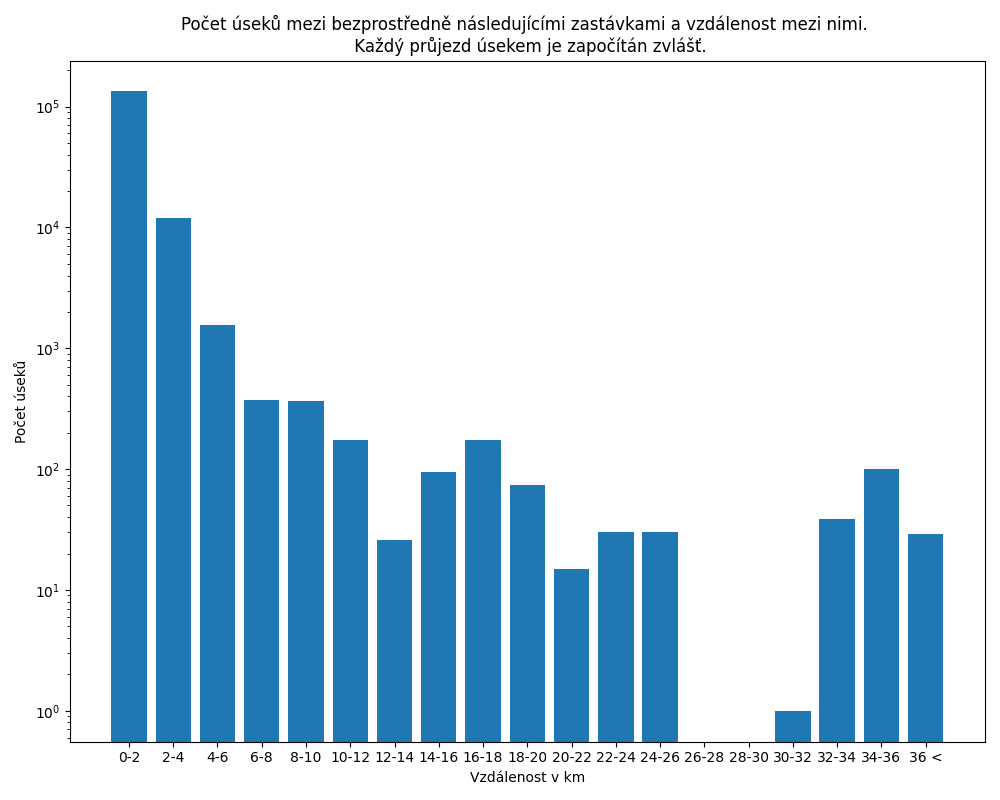
\includegraphics[width=0.6\linewidth]{../img/stop_distances_plot_2020-02-20.png}
  \caption{Graf počtu úseků mezi následujícími zastávkami a vzdálenotí mezi nimi.}
  \label{fig:stop_distances_result}
\end{figure}

\section{Popis problému odhadu zpoždění}

Řešený problém se týká případu, kdy vozidlo projíždí mezi dvěma referenčními body a tato trasa má části, ve kterých vozidlo jede různou rychlostí. Např. vozidlo při vyjíždění z města jede mnohem pomaleji než při jízdě mezi městy a při vjezdu do dalšího města zase zpomalí. Takových úseků, na kterých se rychlost jízdy liší, může být na trase více a nedají se všechny jednoduše detekovat.

\bigbreak

Tato Práce tedy modeluje profily jízd mezi referenčními body. A na základě toho zpřesnˇuje odhad zpoždění. Odhad tímto novým způsobem by měl být mnohem přesnější než současné odhady, které předpokládají, že vozidlo jede konstantní rychlostí po celou dobu jízdy, více rozepsáno v kapitole \ref{subsection:soucasna_reseni_odhadu}. Také je možné brát jako aktuální zpoždění spoje poslední změřené zpoždění při průjezdu nějakým referenčním bodem (zastávkou, návěstidla).

\bigbreak

Přidaná hodnota je tedy v tom, že Práce navrhne takové modely, které nebudou penezalizovat zvyšováním zpožděním za pomalou jízdu v úsecích, které se pomaleji projíždějí vždy. A také naopak zvýhodňovat snížením zpožděním za rychlou jízdu v úsecích, které se obvykle projíždějí rychleji. Pokud bychom se tedy podívali na změny zpoždění na trase mezi dvěma referečními body, v ideálním případně by měli být nulové.

\bigbreak

Pro řešení odhadu toho typu spoždění stačí navrhnout systém na odhadu zpoždění v půběhu jízdy mezi referenčními body z historikých dat jízd.

\bigbreak

Pro vyloučení všech pochybností je hodno uvést, že se naše Práce nesnaží předpovědět zpoždění, které spoj může nabrat vzhledem k dosavadnímu průběhu trasy. Tedy např. nijak nezohledňuje to, že spoj právě stojí v mimořádné koloně a dalo by se tedy předpokládat, že zpoždění bude rychle růst i v následujících minutách. Ale naopak Práce se snaží odhadnou zpoždění v danném bodě na trase vzhledem k obvyklému profilu jízdy. Tedy např. pokud by výše uvažavaná kolona byla pravidelná Práce ji zohlední ve statistických modelech.


\subsection{Příklad nelineárního profilu trasy} \label{subsection:priklad_nelinearni_trasa}

Celé ilustrováno na příkladě jízd mezi dvěma zastávkama K letišti a ZLičín, kde je nelineární profil jízdy vidět velice dobře. Jedná se totiž o trasu přesně odpovídající popisu problému.

\bigbreak

Popsané rozdíly v rychlosti a nelineární profil trasy je patrný na grafu \ref{fig:k_letisti_to_zlicin_3d}. Za povšimnutí táké stojí viditelné zpomalení průjezdů v ranní špičce, 7--9 \footnote{časy jsou v UTC} hodina ráno.

\bigbreak

Tento příklad dále podrobněji analyzován v kapitole \ref{subsubsection:analyza_dat}.

\begin{figure}
  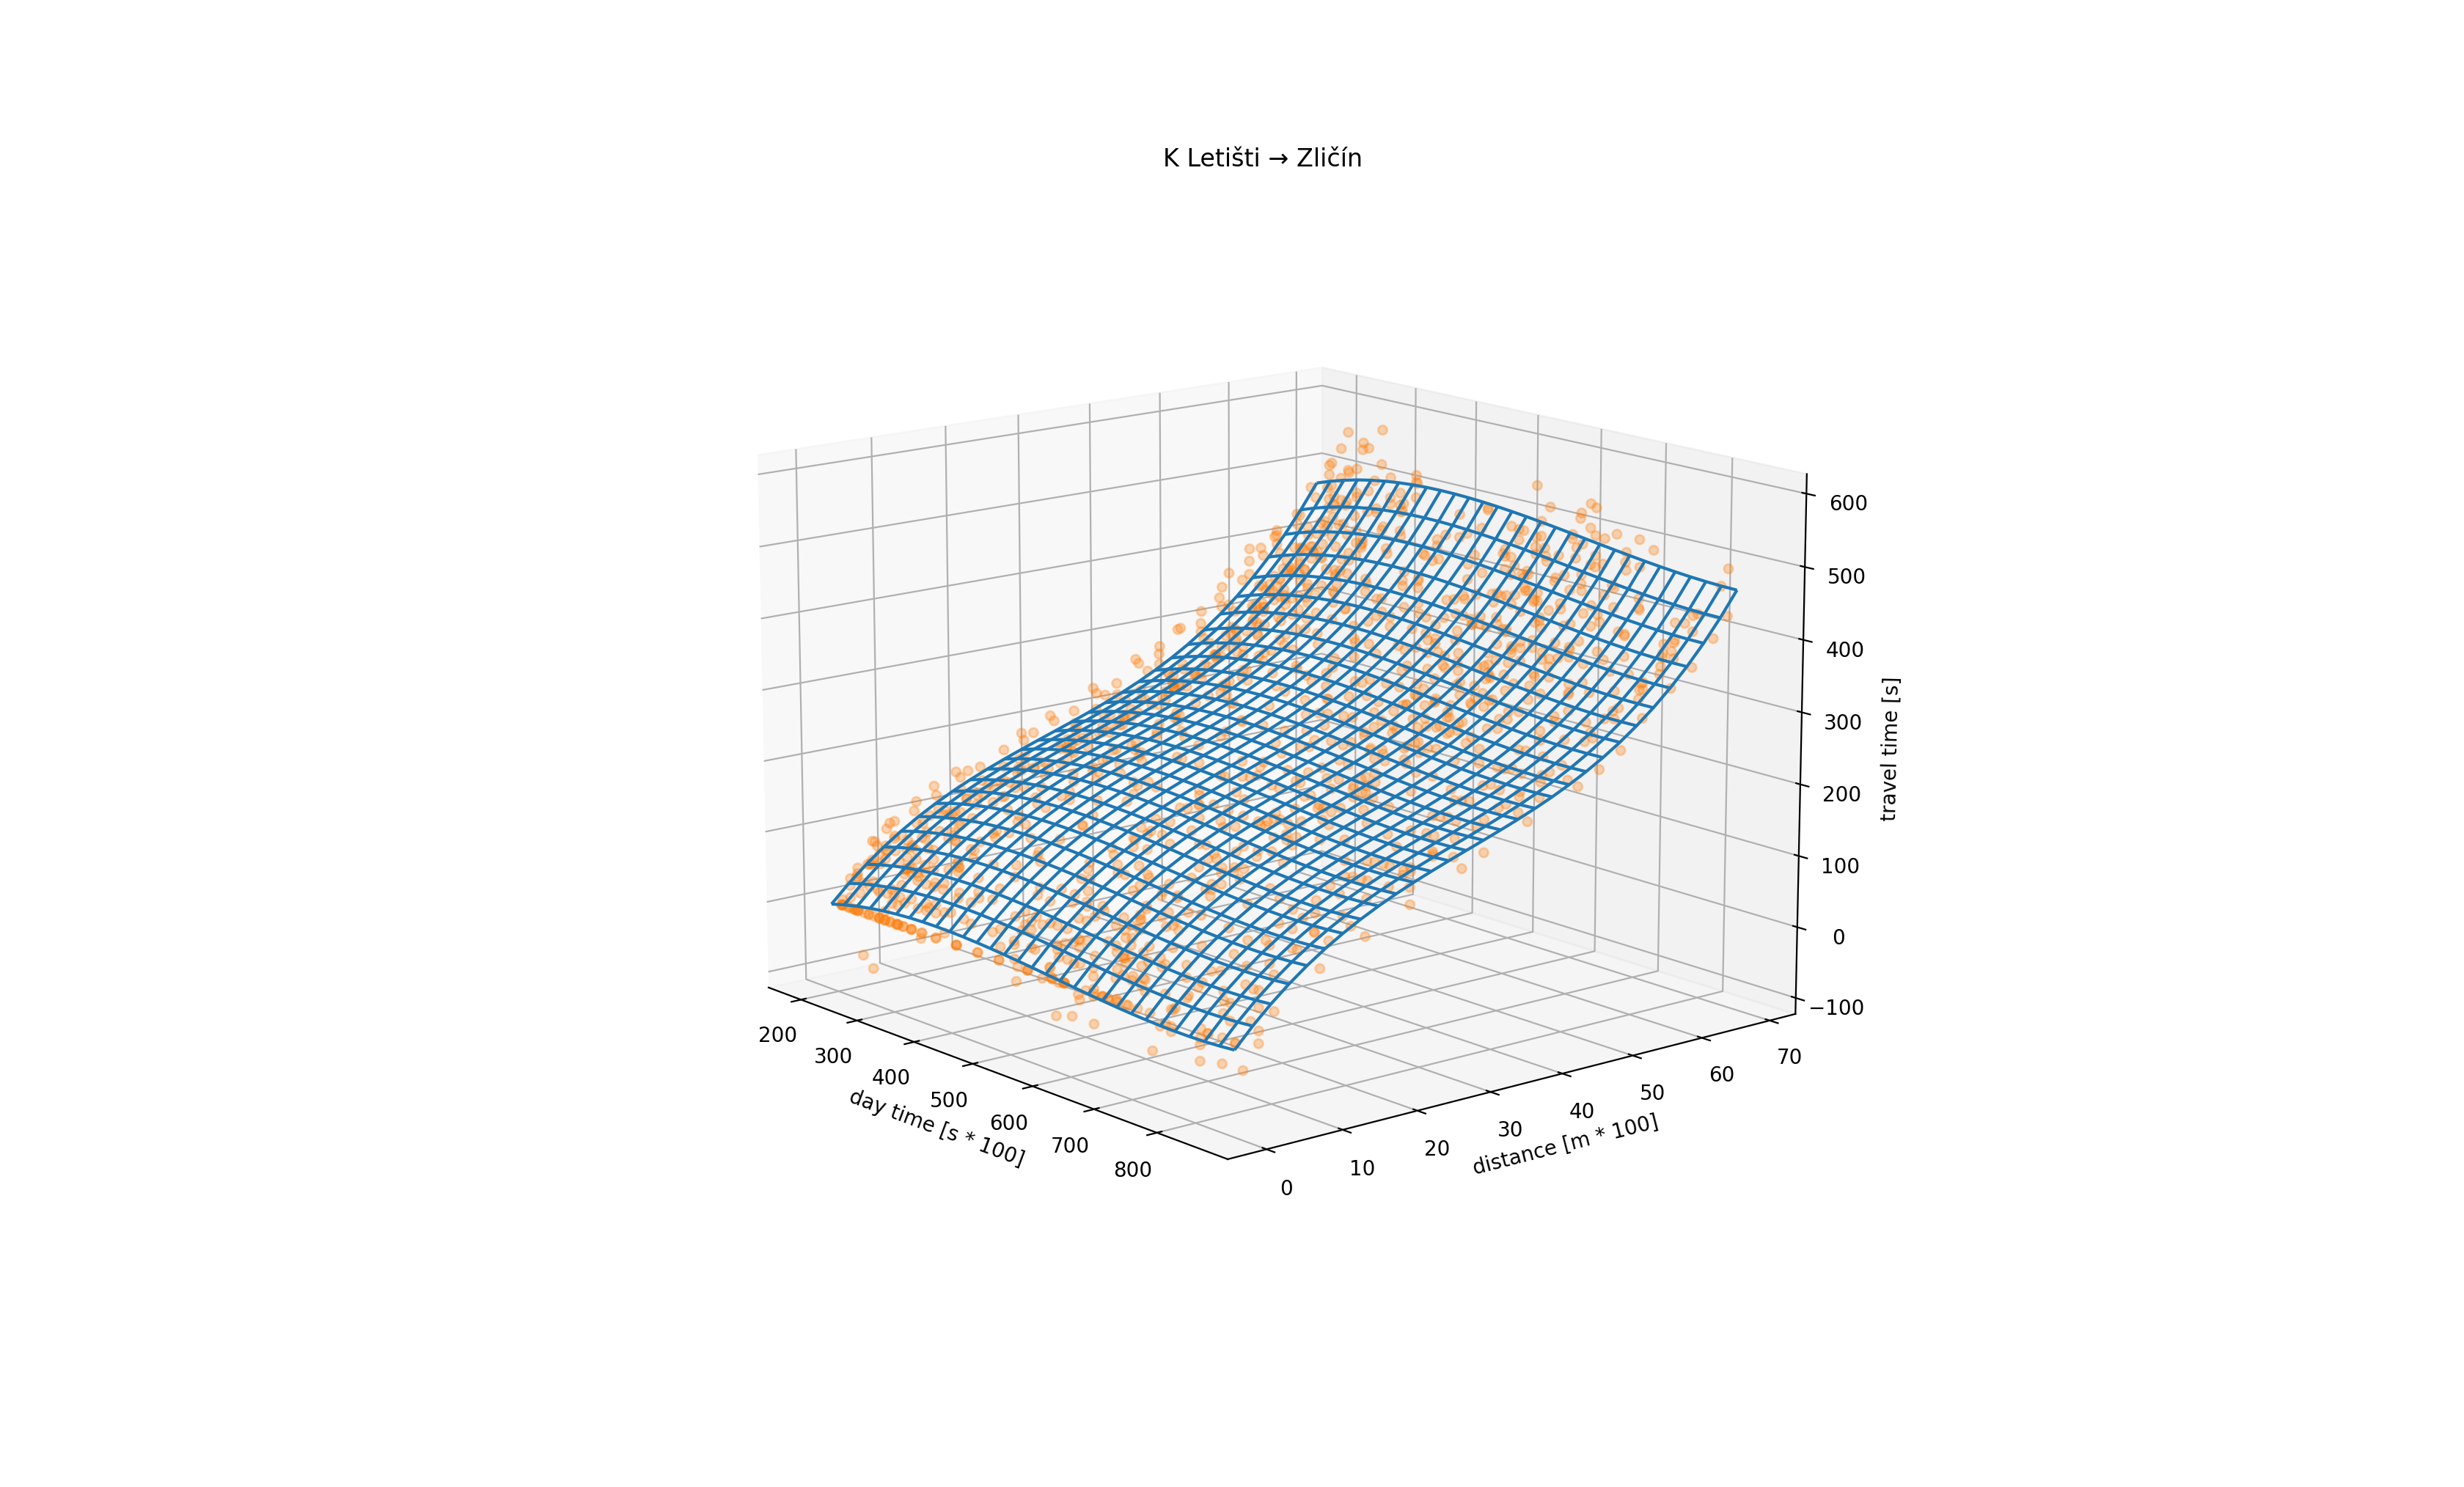
\includegraphics[width=\linewidth]{../img/k_letisti_to_zlicin_3d.png}
  \caption{Modrá plocha značí vymodelovaný profil trasy. Oražové body jsou jednotlivé vzorky polohy vozidel. Data pro graf jsou ze dnů 20.--21. 2. 2020}
  \label{fig:k_letisti_to_zlicin_3d}
\end{figure}

\bigbreak

Na obrázku \ref{fig:k_letisti_to_zlicin_map} je pro bližší představu popsané trasy vidět trasa spoje vykreslená do mapy.

\begin{figure}
	\centering
  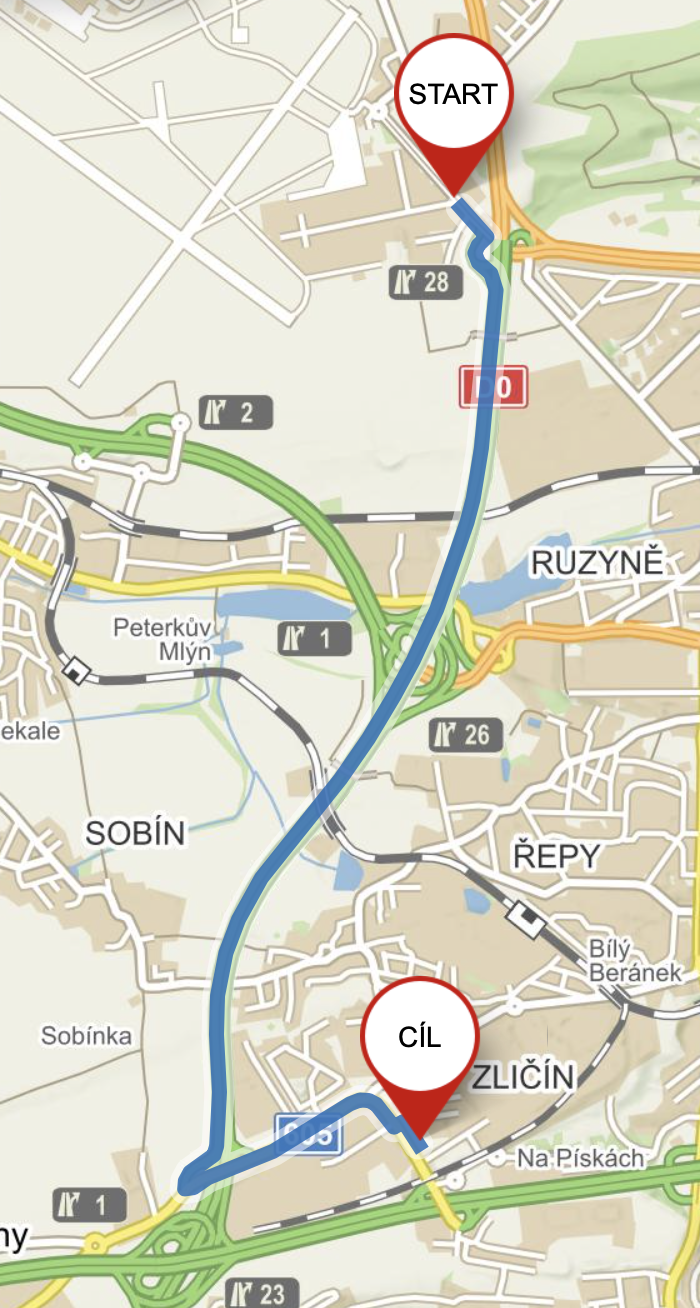
\includegraphics[width=0.3\linewidth]{../img/k_letisti_to_zlicin_map.png}
  \caption{Trasa mezi zastávkama K Letišti a Zličín. Zdroj: mapy.cz}
  \label{fig:k_letisti_to_zlicin_map}
\end{figure}

\subsubsection{Rozbor trasy}

Celá tato trasa má necelých 7 km a její průjezd spojem VHD trvá 10 minut. Prvních 600 metrů je vedeno po obecní komunikaci, přes křižovatku a nájezd na Pražský okruh. Průměrná rychlost vozidel byla 35 km/h\footnote{Počítáno podle vozidel, které poslaly polohu v 600m (resp. 4.9km, resp. 6.6km pro další údaje o rychlosti) vzdálenosti od zastávky. Počet záznamů o poloze vozidel se v různých vzdálenostech liší.}.

\bigbreak

Dále trasa pokračuje přes Pražský okruh rovně až do vzdálenosti 4.9 km od zastávky K Letišti, kde začíná nájezd na ulici Na Radost. Dá se předpokládat, že vozidla se na komunikaci vyšší třídy pohybují rychleji což dokazuje, že na tomto úseku trasy se průměrná rychlost vozidel zvýšila na 63 km/h.

\bigbreak

Poslední úsek se tedy skládá z výjezdu z Pražského okruhu, průjezdu křižovatkou, jízdy po obecní komunikaci a vjezdu do stanice Zličín. Délka úseku je 2 km. Průměrná rychlost za celou trasu se na tomto úseku snížila na 55 km/h. Do této průměrné rychlosti se započítává i jízda ve všech výše popsaných úsecích, tedy skutečná průměrná rychlost v tomto posledním úseku byla výrazně menší.


\subsection{Současná řešení} \label{subsection:soucasna_reseni_odhadu}

Algoritmus na odhad aktuálního zpoždění mezi dvěma referenčními body již exituje a je součástí Datové Platformy -- Golemio, ze kterého se čerpají data pro tuto práci. (Detailní popis dat uveden v kapitole \ref{chapter:analyza_zdroje}.)

\bigbreak

Nicméně tento algoritmus nijak nezohledňuje variabilitu profilu trasy. Totiž v tomto řešení je nahlíženo na postup vozidla na trase jako na lineární funkci vůči času. Je ovšem zřejmé, že rychlost vozidel není konstantní, neboli doba jízdy není linárně závislá na ujeté vzdálenosti.

\bigbreak

TODO obrazek linearniho modelu

\bigbreak

Proto je potřeba tento odhad zpřesnit, což je cílem naší práce. K tomuto cíli jsme byli nasměrováni v rámci schůzky s pracovníky společnosti OICT, kde bylo řečeno, že toto je problém současného řešení, který je potřeba vyřešit.


\section{Analýza zdroje dat} \label{chapter:analyza_zdroje}

V této kapitole je popsán zdroj real-timových dat o polohách vozidel využívané v této práci.

\subsection{Přístup k datům}

Vozidla vysílají data o své poleze při různých událostech. Zejména pak při brždění, rozjezdu, vyhlášení zastávky, nebo jinak každých 20 sekund\footnote{Řečeno zaměstnancem OICT na schůzce 4. 5. 2019}.

\bigbreak

Taková data pak přímo putují k provozavoateli systému na monitorování vozidel, kterým je společnost \gls{kapsch} jakožto partner \gls{ropid}. Ten však tato data zpracovává a posílá ke zveřejnění na platformě Golemio. Bohužel při tomto procesu zpracování se vytratí informace o události v jáké byla data pořízena. Tedy informace o příjezdu nebo odjezdu ze zastávky jsou zjistitelné pouze z \gls{gps} souřadnic a následném odhadu pozice vozidla na trase dané linky.

\bigbreak

Po té co jsou tyto data přeneseny do společnosti Operátor ICT by měla být zveřejněna, nicméně data ve výše popsané podobě jsou poměrně chudá, proto je k nim přidáno více atributů. Jedná se o dopočet poslední projeté zastávky, ujeté vzdálenosti od výchozí stanice, zpoždění v poslední zastávce.

\bigbreak

 Z pohledu této práce je nejzajímavější informace o vzdálenosti, kterou vozidlo urazilo od jeho výchozí zastávky. Dále jsou přidána data o jízdních řádech a zastávkách jejichž původcem je \gls{ropid}.

\bigbreak

Real-time data o polohách, která jsou již neplatná (zastaralá) se neposílají (posílá vždy pouze nejaktuálnší informace) a i z Datové platformy jsou data po pár minutách nenávratně smazána.

\subsubsection{Dokumentace}

Na úvod je nutné poznamenat, že datová platforma je stále ve vývoji a formát dat se může měnit. S tím mohou přicházet určité výpadky a problémy. K jednomu takovému výpadku došlu i při vývoji této práce, kdy po dobu 14 dnů platfomarma vůbec neodpovídala na dotazy nebo vracela prázdné datasety.

\bigbreak

Současně s využívanou verzí \gls{api}, je nasazená i pokročilejší \gls{api} ve verzi 2, které obsahuje více informací a je přehledněji upravena. Nicméně při zahájení vývoje této práce nebyla verze 2 k dispozici, proto jsou využívána data pouze ze starší verze.

\bigbreak

Oficiální uživatelská dokumentace datové platformy\footnote{Golemio: https://golemioapi.docs.apiary.io} je poměrně zastaralá sama o sobě tak, že aktuální sada parametrů jí neodpovídá a neobsahuje žádné popisy nebo vysvětlení dat. Proto vysvětlení jednotlivých atributů se zakládá na intuitivním pochopení nebo vyplynulo z jednání se správci platformy. V následujících kapitolách bude popsán formát dat, tak jak přichází ze zdroje. Ten se může od oficiálně vystavené dokumentace lišit. A také budou popsány pouze atributy využívané v této práci nebo zajímavé pro její budoucí rozvoj.

\bigbreak

Každá datová sada je exportována ve formátu \gls{geojson} pokud se jedná o geografická data, nebo jinak ve formátu \gls{json}. Přistupuje se k nim přes jednotné webové rozhraní pomocí \gls{http} požadavku daného \gls{url} adresou a jeho hlavičkou.

\bigbreak

Ačkoli se dokumentace tváří tak, že data jsou exportována ve formátech \gls{json} nebo \gls{geojson}, většinou formát dat není přesně podle specifikace těchto formátů. Například může být uveden atribut \verb"wheelchair_accessible", který je typu \verb"bool" a je nastaven na hodnotu \verb"True", nicmně podle specifikace se tyto hodnoty píší s malým písmenem\footnote{V průběhu tvorby této práce byla chyba opravena.}. Pro tuto práci to sice nepředstavuje komplikaci, protože tento atribut není potřeba, ale mohlo by se stát, že některé parsery \gls{json}u vyhodnotí řetězec jako nevalidní a skončí chybou.

\bigbreak

Celá datová platforma Golemio je pojatá jako Open Source projekt\footnote{Programátorská dokumentace je dostupná na https://operator-ict.gitlab.io/golemio/documentation/}. Tedy je možné její zdrojový kód vylepšit či opravit nebo také čtením kódu detailně porozumnět jak zde popisované zpracování dat funguje. Avšak takový rozbor zdrojového kódu je mimo rozsah této práce.

\subsubsection{Pozice vozidel}

Ze zveřejněných dat na této platformě jsou nejdůležijtější data pro tuto práci polohy vozidel. Jelikož se jedná o real-time data, data rychle zastarávají a je nutné je velmi často aktualizaovat.

\bigbreak

Využívané atributy jsou:

\begin{itemize}
	\item \verb-coordinates- aktuální \gls{gps} souřadnice vozidla

	\item \verb-origin\_timestamp- čas zachycení polohy vozidla, v časovém pásmu \gls{utc}

	\item \verb-gtfs\_trip\_id- unikátní identifikátor tripu pro spárování s jízdním řádem

	\item \verb-gtfs\_shape\_dist\_traveled- vzdálenost vozidla uražená od začátku jízdy v metrech

	\item \verb-delay\_stop\_departure- zpoždění zachycené při odjezdu z poslední projeté zastávky v sekundách
\end{itemize}.

Příklad dat popisující aktuální polohu vozidla, na kterém je možno vidět strukturu dat i další atrubuty. Řada z nich je pro tuto práci zbytečná. Dále je možno si povšimnout atrubutu \verb-all\_positions-, který obsahuje všechny zaznamenané pozice daného vozdila na jeho aktuální trase, tento atribut je z důvodů objemu dat volitelný a pro tuto práci se nevyužívá.

\begin{code}[frame=none]
"geometry":{
  "coordinates":[14.91724,50.41881],
  "type":"Point"
},
"properties":{
  "trip":{
    "cis_agency_name":"ČSAD Česká Lípa",
	"cis_id":"260467",
	"cis_number":3008,
	"cis_order":2,
	"cis_parent_route_name":"467",
	"cis_real_agency_name":"ČSAD Česká Lípa",
	"cis_short_name":null,
	"cis_vehicle_registration_number":1073,
	"gtfs_route_id":"L467",
	"gtfs_route_short_name":"467",
	"gtfs_trip_id":"467_252_200105",
	"id":"2020-02-23T18:50:00Z_260467_467_3008",
	"start_cis_stop_id":30107,
	"start_cis_stop_platform_code":"A",
	"start_time":"19:50:00",
	"start_timestamp":"2020-02-23T18:50:00.000Z",
	"vehicle_type":4,
	"wheelchair_accessible":true
  },
  "last_position":{
    "bearing":20,
	"cis_last_stop_id":21393,
	"cis_last_stop_sequence":28,
	"delay":261,
	"delay_stop_arrival":null,
	"delay_stop_departure":287,
	"gtfs_last_stop_id":"U3389Z1",
	"gtfs_last_stop_sequence":30,
	"gtfs_next_stop_id":"U2987Z30",
	"gtfs_next_stop_sequence":31,
	"gtfs_shape_dist_traveled":"64.1",
	"is_canceled":false,
	"lat":"50.41881",
	"lng":"14.91724",
	"origin_time":"21:29:37",
	"origin_timestamp":"2020-02-23T20:29:37.000Z",
	"speed":20,
	"tracking":2,
	"trips_id":"2020-02-23T18:50:00Z_260467_467_3008"
	},
  "all_positions":{
    "features":[],
	"type":"FeatureCollection"
  }
},
"type":"Feature"

\end{code}

\subsubsection{Jízdy}

Dále jsou k dispozici data o každém spoji. To je popis trasy vozidla, včetně zastávek a časů příjezdů a odjezdů do/z nich. Také může být vyžádáno k informacím o jízdě připojit celý detailní nákres trasy, tj. lomená čára kopírující celou trasu daného tripu po povrchu Země.

\bigbreak

 Míra unikátnosti identifikátorů těchto tripů je předmětem dohadů a zřejmě jsou pod správou plánovačů \gls{vhd}, nicméně pro účely této práce může být předpokládáno, že každá jízda má vlastní jízdní řád, který se váže na čas a každá jízda jede nejvýše jednou za den.

\begin{itemize}
	\item \verb-trip\_headsign- nápis na čele vozidla, typicky cílová stanice

	\item \verb-route\_id- číslo linky

	\item \verb-trip\_id- unikátní identifikátor tripu pro spárování s real-time daty, pravděpodobně odpovídá atributu \verb"gtfs\_trip\_id"


\end{itemize}

Navíc s každým tripem může být vyžádáno zaslání seznamu zastávek, kterýma projíždí. Zde jsou k dispozici informace vázající se k danému průjezdu zastávkou. Každá uvená zastávka s sebou nese i kompletní informaci o sobě, tedy má stejnou informační hodnotu jako samostatný dotaz na jednotlivé zastávky z datové sady zastávek.

\subsubsection{Zastávky}

\begin{itemize}
	\item \verb-arrival_time- čas příjezdu spoje do zastávky

	\item \verb-departure_time- čas odjezdu spoje do zastávky

	\item \verb-shape_dist\_traveled- vzdálenost zastávky na trase od výchozího bodu daného tripuv metrech

	\item \verb-stop_id- unikátní indetifikátor zastávky

	\item \verb-coordinates- \gls{gps} souřadnice zastávky, často \verb"null", je třeba využít atributy \verb"stop\_lat" a \verb"stop\_lon"

	\item \verb-stop_name- název zastávky
\end{itemize}

\bigbreak

Příklad dat popisujících jednu jízdu včetně zastávek. Seznam zastávek a body trasy jsou zkráceny vzhledem k objemu dat.

\begin{code}[frame=none]
"bikes_allowed":2,
"block_id":"",
"direction_id":1,
"exceptional":1,
"route_id":"L421",
"service_id":"1111100-1",
"shape_id":"L421V4",
"trip_headsign":"Kolín,Nádraží",
"trip_id":"421_225_191114",
"trip_operation_type":1,
"trip_short_name":"",
"wheelchair_accessible":2,
"stop_times":[{
  "arrival_time":"14:14:00",
  "arrival_time_seconds":null,
  "departure_time":"14:14:00",
  "departure_time_seconds":null,
  "drop_off_type":"0",
  "pickup_type":"0",
  "shape_dist_traveled":0,
  "stop_headsign":"",
  "stop_id":"U2033Z5",
  "stop_sequence":1,
  "timepoint":null,
  "trip_id":"421_225_191114",
  "stop":{
    "geometry":{
      "coordinates":[
        null,
        null
      ],
      "type":"Point"
    },
    "properties":{
      "level_id":"",
      "location_type":0,
      "parent_station":"",
      "platform_code":"5",
      "stop_code":null,
      "stop_desc":null,
      "stop_id":"U2033Z5",
      "stop_lat":49.87486,
      "stop_lon":14.9078,
      "stop_name":"S\u00e1zava,Aut.st.",
      "stop_timezone":null,
      "stop_url":"",
      "wheelchair_boarding":0,
      "zone_id":"5"
    },
    "type":"Feature"
  },
  ...
],},
"shapes":[{
  "geometry":{
    "coordinates":[
      14.90778,
      49.87494
    ],
    "type":"Point"
  },
  "properties":{
    "shape_dist_traveled":0,
    "shape_id":"L421V4",
    "shape_pt_lat":49.87494,
    "shape_pt_lon":14.90778,
    "shape_pt_sequence":1
  },
  "type":"Feature"
},
...
]

\end{code}

\subsection{Analýza statických dat}

Sběr dat probíhal ve dnech 20.--23. 2. 2020.

\bigbreak

Data byla přebírána pouze z dat o každé jednotlivé jízdě a aktuálních poloh vozidel stahovaných každých 20 sekund. Tedy pokud určitou zastávkou žádný spoj neprojel nebo se uložení spoje z důvodu neúplných dat nezdařilo, může nějaká zastávka v databázi chybět. Stejně tak mohou chybět i nějaké spoje. Nejčastěji chybějící požadovaná data jsou informace o spoždění spoje v poslední zastávce, zcela nenalezený spoj ve zdroji dat a tedy chybějící jízdní řád. Nicméně jedná se o zanedbatelné množství spojů. Práce totiž nemůže počítat s poškozenými daty a není jejím úkolem držet všechny zastávky, ale pouze ty kterými nějaký spoj projíždí. To z důvodu přehlednosti zastávek při vizualizaci, kde ukazovat nepoužívané zastávky nemá smysl a také pro odhady zpoždění nedává smysl počítat něco pro zastávku, která není obsluhovaná.

\subsubsection{Zastávky} \label{subsubsection:zastavky}

Do databáze bylo celkem vloženo 5820 nástupišť, které náleží celkem 2961 zastávkám. Ale naprostá většina (74 \%) zastávek jsou párová, tedy mají pouze 2 nástupiště. Jednosměrných zastávek je 18 \%, zastávek se 3 nástupišti jsou 3 \%. Nejvíce nástupišť mají stanice Slaný Aut. nádr. (14), Černý Most (12), Kladno Autobusové nádraží (11).

\subsubsection{Jízdy}

Celkem bylo nalezeno 12788 spojů, z nich naprostá většina vyjela opakovaně v následující den\footnote{Ze všech vypravených jízd ve dnech 20. 2. 2020 (9334) a 21. 2. 2020 (9428) jich 9051 bylo označeno ve zdrojových datech stejným identifikátorem, tedy z našeho pohledu sdílely jízdní řád a trasu.}.

\subsubsection{Vstupní soubory} \label{subsubsection:vstupni_soubory}

Pro testovací účely bylo celkem pořízeno 15 794 obrazů dopravní situace záznamenávající aktuální polohy vozidel.

\bigbreak

Pro stahování těchto souborů byl využit script napsaný v jazyce Bash, který po dobu 4 dnů periodicky každých 20 sekund stáhl aktuální obraz poloh vozidel. Tento stažený dokument pak uložil v komprimovaném formátu a označil časem stažení. Tento script běžel na počítači, který pro účely této práce zapůjčil k využití pan profesor Jakub Klímek, jemuž tímto děkuji.

\begin{code}[frame=none]
#!/bin/sh

cur_file="current_json_file.json";

while :
do
  curl -s --header "Content-Type: application/json; charset=utf-8" \
  --header "access token" \
  'https://api.golemio.cz/v1/vehiclepositions' > "$cur_file";

  if [ 0 -ne $? ];
  then
    today=`date +%Y-%m-%dT%H.%M.%S`;
    echo "Curl failed $today" >> downloader.log;
    sleep 19;
    continue;
  fi

  today=`date +%Y-%m-%dT%H.%M.%S`;
  tar -czf "../raw_data-2/${today}.tar.gz" $cur_file;
  echo "File ${today}.tar.gz saved." >> downloader.log
  sleep 20

done

\end{code}

\bigbreak

Z celkového počtu nalezenách spojů vyplývá, že počet nově nalezených spojů v jednom obrazu je méně než jeden. Kompletní histogram počtu souborů poloh vozidel, které obsahují určitý počet nově objevených spojů je zobrazen na grafu \ref{fig:vehicle_pos_x_new_trips}.

\begin{figure}
	\centering
  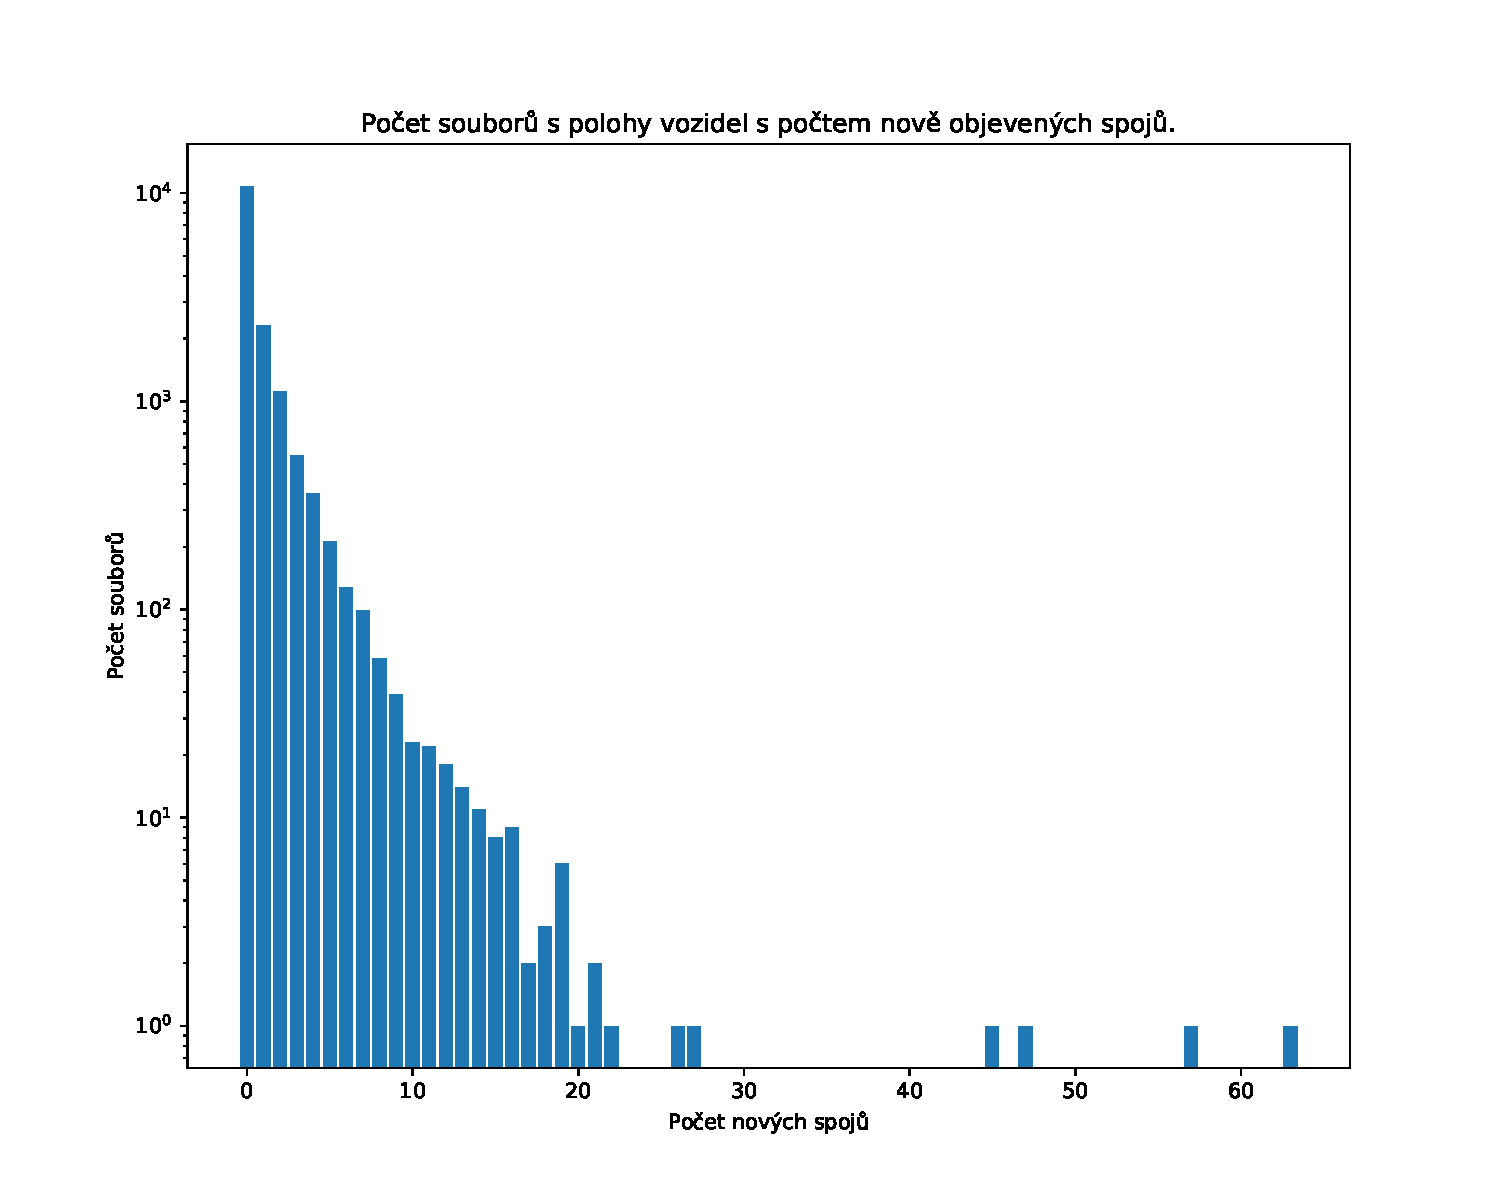
\includegraphics[width=0.7\linewidth]{../img/vehicle_pos_x_new_trips}
  \caption{Počet souborů s početem nově nalezených spojů v nich.}
  \label{fig:vehicle_pos_x_new_trips}
\end{figure}

\bigbreak

Maximální počet vozidel obsažených v jednom souboru je méně něž 800. Kompletní histogrtam počtu souborů s počtem vozidel celkem v jednom souboru je na grafu \ref{fig:vehicle_pos_x_all_trips}. Z tohoto grafu vyplývá, že velká většina vstupních souborů z celkového počtu 15793 obsahuje do 200 vozidel v každém souboru.

\bigbreak

Avšak ne všechna vozidla v každém souboru jsou nová nebo dostala změněny oproti předešlému záznamu. To z důvodu, že je zdroj dat nastaven tak, aby vysílal polohu vozidla jako aktuální, i když už je zastaralá několik minut. V takovém případě se zpracovává vzorek volohy vozdila stále dokola.

\begin{figure}
	\centering
  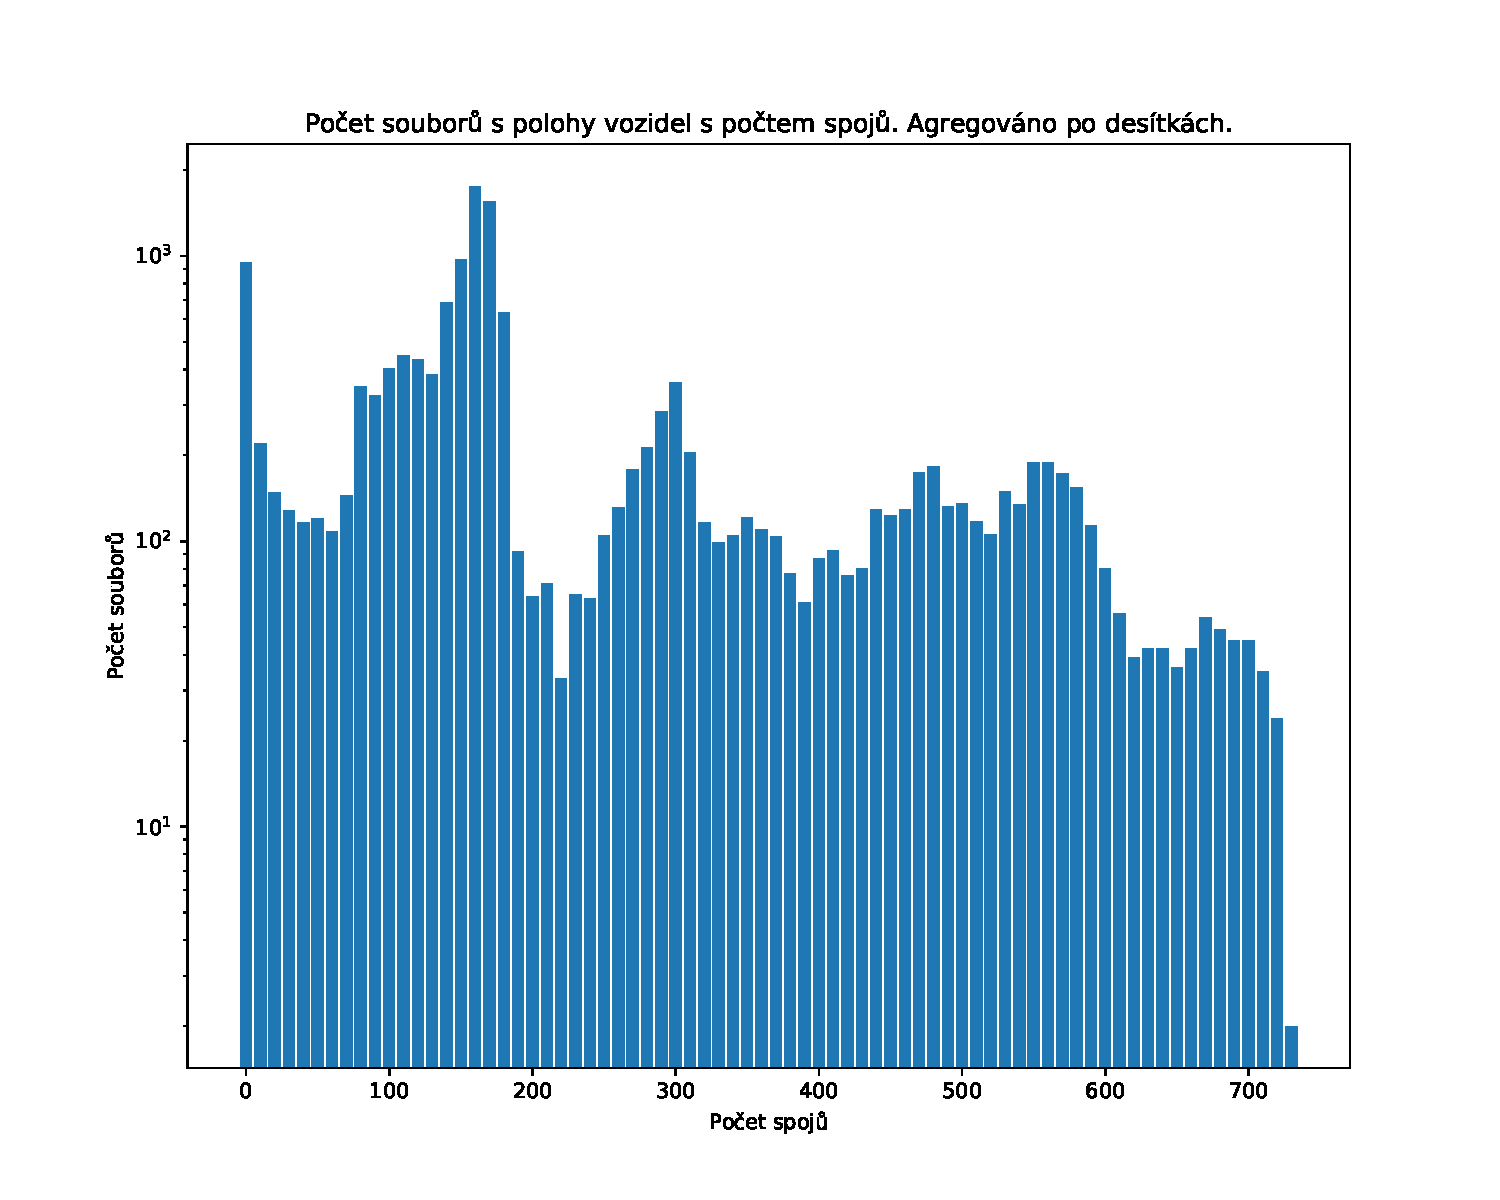
\includegraphics[width=0.7\linewidth]{../img/vehicle_pos_x_all_trips}
  \caption{Počet souborů s početem nově nalezených spojů v nich.}
  \label{fig:vehicle_pos_x_all_trips}
\end{figure}

\bigbreak

Další rozbor dat na grafu \ref{fig:stop_distances_result} a v kapitole \ref{TODO:statistika}.




\section{Analýza vizualizačních nástrojů}

Jak bylo řečeno v úvodu, součástí práce je i vizualizace spočítaných dat.

\bigbreak

To bude provedeno formou front endové aplikace, která zobrazuje mapu a do ní zanáší data o vozidlech \gls{vhd}. Funkční požadavky této aplikace jsou inspirované již existujícími řešeními tohoto problému.

\subsection{Mapové podklady}

Jak vyplývá z funkčních požadavků data budou zobrazována v mapě. Mapu si samozřejmě nebudeme kreslit sami, ale využijeme jedno z již existujcích řešení, které umožňuje zobrazení mapy a do ní zanést vlastní data. Takové služby mohou být provozovatelem zpoplatněny, ale pro naše demonstrační účely, kdy budeme využívat tuto službu velmi málo, bývá od poplatků většinou upoštěno.

\bigbreak

Jedním z těchto poskytovatelů je společnost Google, která má propracované mapové podklady a prostřednictvím služby Google Maps a poskytuje pro tuto práci požadovanou službu nazývanou Google My Maps\footnote{https://www.google.com/maps/about/mymaps/}.

\bigbreak

Další platformou je Mapbox\footnote{https://www.mapbox.com}, který poskytuje s využitím dalších knihovem velmi podobné služby jako Google My Maps. Nicméně narozdíl od Googlu využívá jako mapový podklad \gls{osm} {otevřená geografické data}.

\bigbreak

Protože smyslem práce je v co největší míře využít otevřená data je žádoucí využít právě službu Mapbox.

\subsection{Současná řešení} \label{subsection:soucasna_reseni_front_end}

Vizualizaci vozidel \gls{vhd} do mapy již nabízí několik portálů. Všechny jsou však poměrně strohé.

\subsubsection{Golemio}

Takovou mapu zobrazuje i samotný provozavatel datové platformy. Nicméně nejsou zde vidět ani čísla linek zobrazených autobusů, natož pak nějaké další informace. Příklad vizualizace je uveden na obrázku \ref{fig:golemio_result}.

\begin{figure}
	\centering
  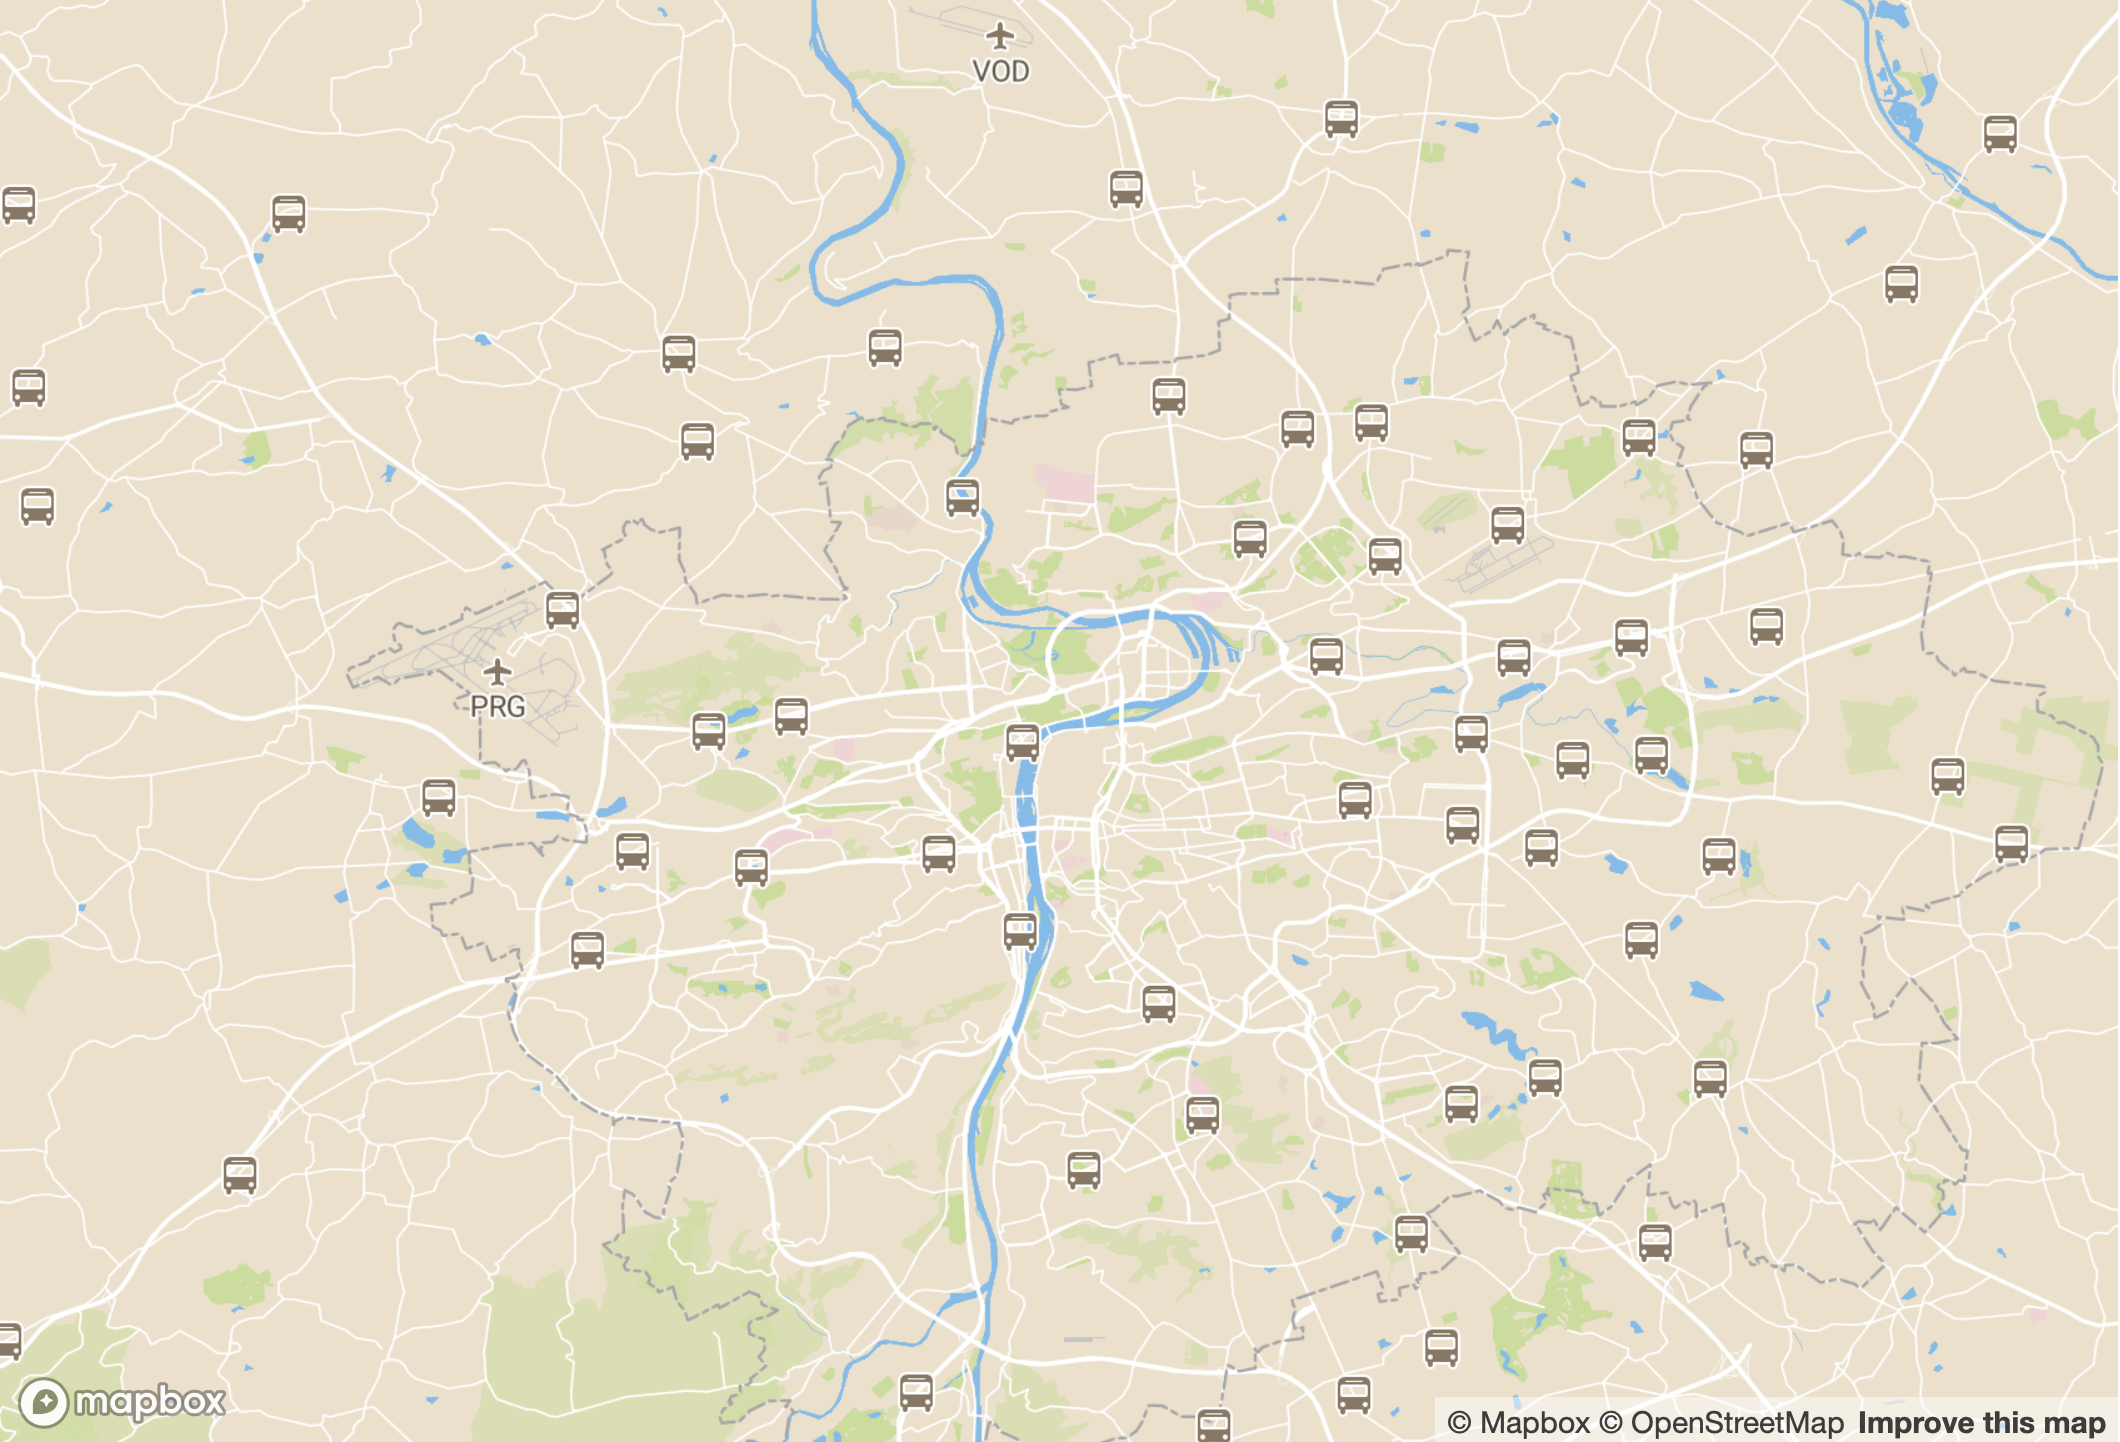
\includegraphics[width=0.5\linewidth]{../img/golemio_mapa.png}
  \caption{Mapa z golemio.cz.}
  \label{fig:golemio_result}
\end{figure}

\subsubsection{Tram-bus}

Dalším poskytovatelem je portál tram-bus, který si vede o něco lépe. Ukazuje směr jízdy vozidel, čísla linek a po kliknutí informace o zpoždění a nejbližší zastávky. Pozn.: na mapě již jsou vidět spoje \gls{dpp}, protože v době psaní této práce již byly data veřejné. Příklad vizualizace je uveden na obrázku \ref{fig:tram-bus_result}.

\begin{figure}
	\centering
  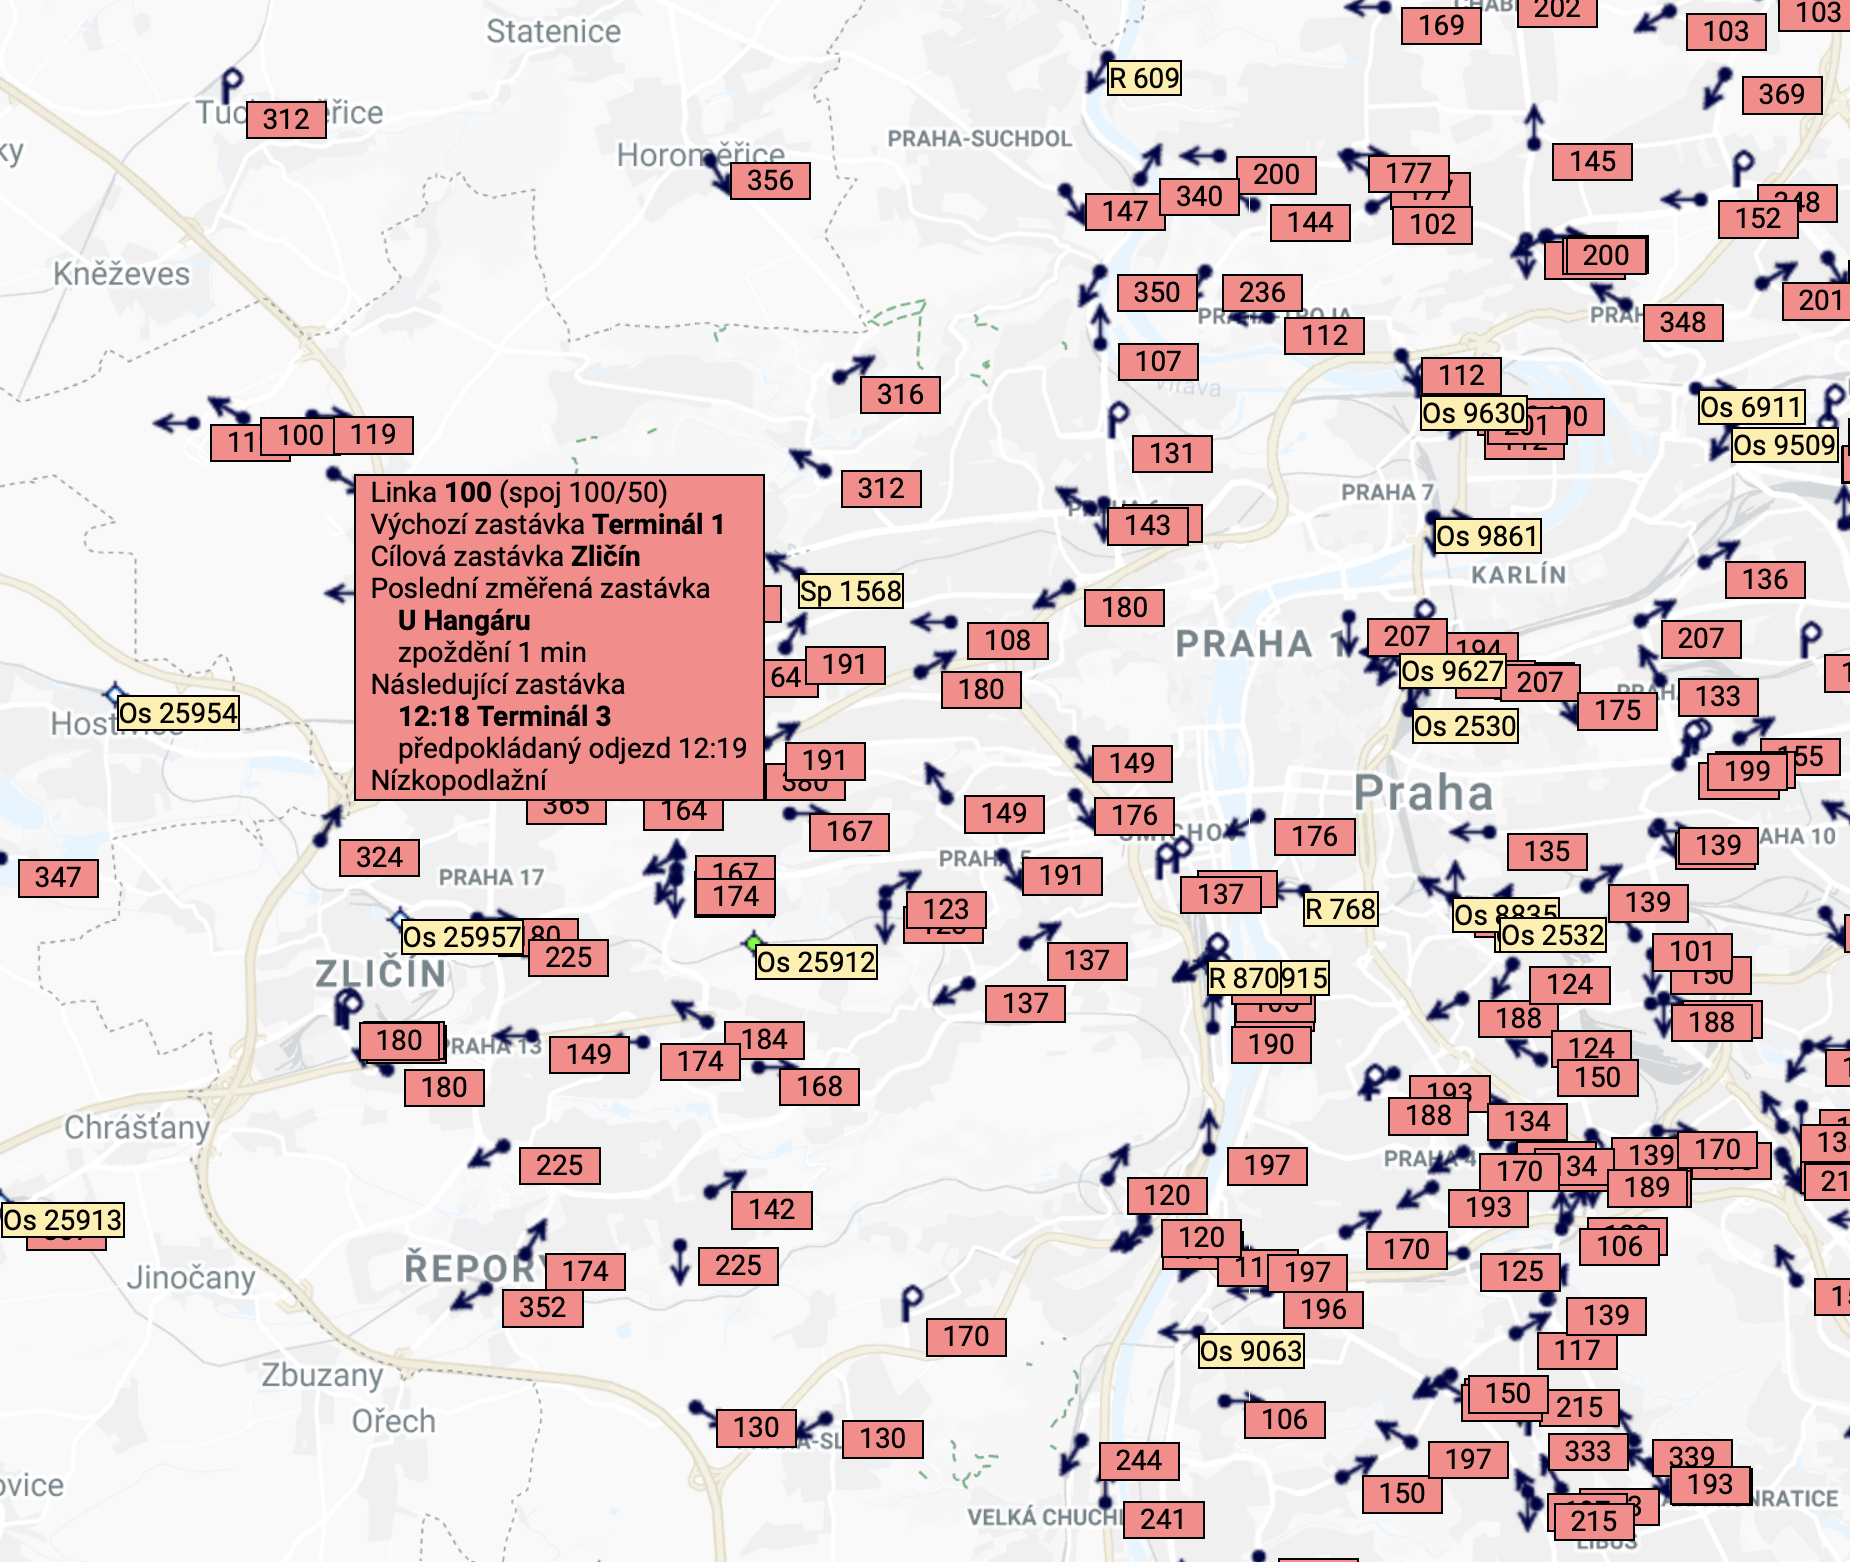
\includegraphics[width=0.5\linewidth]{../img/tram-bus_mapa.png}
  \caption{Mapa z www.tram-bus.cz.}
  \label{fig:tram-bus_result}
\end{figure}

\subsubsection{\gls{idsjmk}}

Mimo Prahu je velice pěkně udělaná aplikace pro zobrazení vozidel \gls{idsjmk} (Integrovaný dopravní systém Jihomoravského kraje). Ten ihned po načtení stránky zobrazuje všechny dobravní prostředky, tedy tramvaje, autobusy a vlaky vše s čísly linek. Dále pak umožňuje po kliknutí na vybraný spoj zobrazit více informací včetně jízdního řádu. Příklad vizualizace je uveden na obrázku \ref{fig:idsjmk_result}.

\bigbreak

Tato aplikace je po vizuální i funkční stránce dobrou inspirací pro tvorbu aplikace v této práci.

\begin{figure}
	\centering
  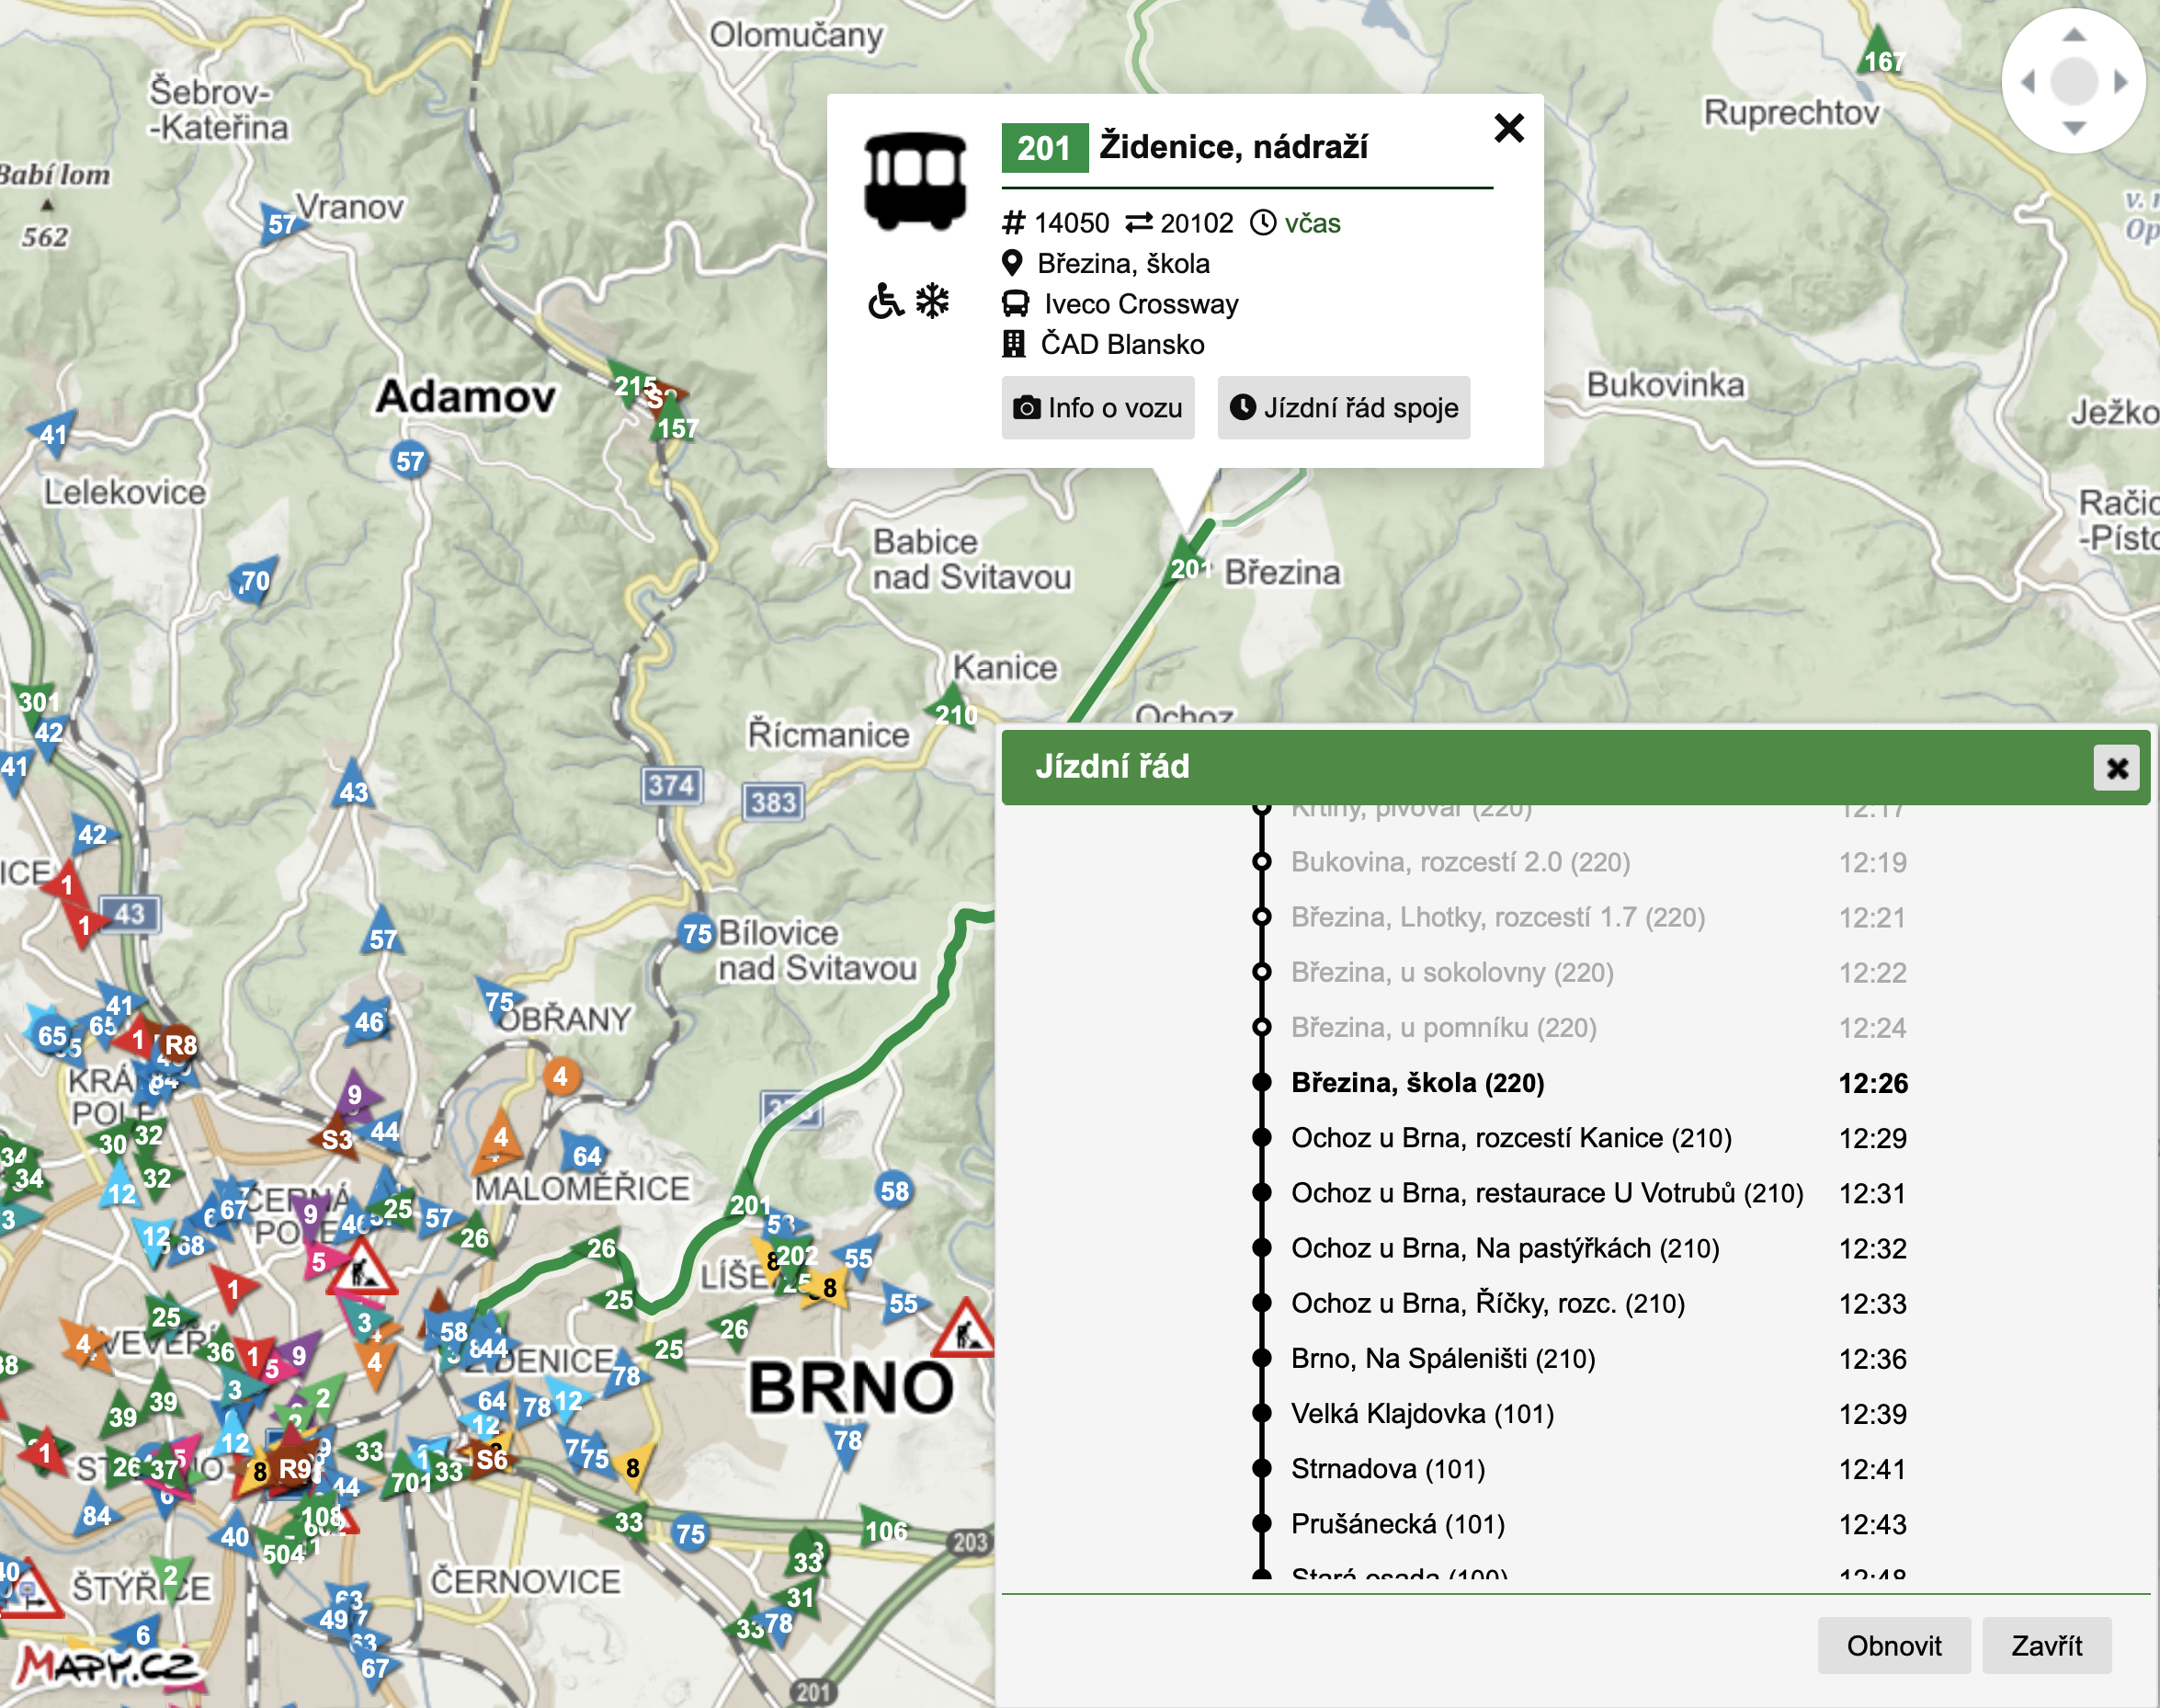
\includegraphics[width=0.5\linewidth]{../img/idsjmk_mapa.png}
  \caption{Mapa z mapa.idsjmk.cz.}
  \label{fig:idsjmk_result}
\end{figure}

%%% Fiktivní kapitola s ukázkami sazby

\chapter{Návrh řešení}

V této kapitole je popsáno technické řešní uvedených problémů.

\section{Odhad zpoždění}

\subsection{Funkční požadavky}

Popsaný odhad změny zpoždění na trase mezi dvěma referenčními body je nutné počítat v co nejkratším čase tak, aby cestující byli dobře informování o stavu jejich spoje a mohli tyto informace využít např. při dobíhání spoje. A proto je potřeba zpracovávat data okamžitě po jejich vydání, spočítat odhad zpoždění a vystavit tato data veřejně. Vzhledem k tomu, že tato data velmi rychle zastarávají je nutné provádět tento proces co možná nejrychleji\footnote{Průměrná doba jízdy spoje mezi zastávkami je cca 5 min. Rozložení počtu úseků mezi zastávekami k délce jízdy mezi nimi je závislé a podobné rozložení vůči vzdálenosti ilustrované na grafu\ref{fig:stop_distances_result}.}.

\bigbreak

Data o polohách vozidel VHD v Datové platfomě jsou aktualizována každých 20 sekund\footnote{Řečeno zaměstnancem OICT na schůzce 4. 5. 2019}. Navíc neplatné (aktualizované) data o polohách se již neposílají. Tedy pro minimalizaci rychlosti zastarávání dat a získání všech existujících vzorků dat o polohách je nutné data stahovat nejpozději každých 20 sekund.

\bigbreak



\section{Vizualizace dat}

\subsection{Funkční požadavky}

Součástí práce je i vizualizace spočítaných dat.

\ bigbreak

To bude provedeno formou front endové aplikace, která zobrazuje mapu a do ní zanáší data o vozidlech VHD. Funkční požadavky této aplikace jsou inspirované již existujícími řešeními tohoto problému, ty jsou dále rozebrány v kapitole \ref{chapter:soucasna_reseni_front_end}

\subsection{Funkční požadavky}

\begin{itemize}
	\item

	\item Aplikace vykreslí interaktivní mapu Prahy a širšího okolí, kterou bude možné posouvat či zoomovat. V této mapě budou zobrazeny vozidla na aktuálních pozicích a budou se automaticky posouvat po mapě, tak jak se pohybují ve skutečnosti.

	\item Po kliknutí na vozidlo se zobrazí jeho celá trasa včetně zastávek a jeho dopočítaného zpoždění.

	\item Po kliknutí na zastávku se zobrazí seznam spojů, které budou projíždět vybranou zastávkou a jejich trasy se vykreslí do mapy.

	\item Celá aplikace bude postavena na principu server -- client. Tedy serverová strana se postará o přístup k otevřeným datům o vozidlech a jejich uložení a také obsluhu požadavků klienta. Klientská část bude webová stránka poskytující služby popsané výše. Měla by být schopná zobrazit řádově tisíce vozidel.
\end{itemize}

\subsubsection{Nefunkční požadavky}

\begin{itemize}
	\item Serverová část bude napsaná v jazyce Python 3.

	\item Webová část bude napsaná pomocí jazyků pro webové technologie, převážně v JavaScriptu.

	\item Pro vykleslení mapy bude využita služba Mapbox.

	\item Ukládání dat na serverové straně bude řešeno MySQL databází.

	\item Pro algoritmus odhadu zpoždění na zákldě historických dat budou využity různé knihovny pro jazyk Python 3. Zejména pak scikit-learn a alphashape.

\end{itemize}

\subsubsection{Proces běhu aplikace}

Jak je již zmíněno aplikace bude využívat historická data, tedy bude nutné nechat aplikaci tato data nějakou dobu sbírat. Pro efektivní odhady by bylo vhodné mít uložené historické polohy vozidel alespoň z uplynulých několika týdnů.

\bigbreak

Avšak již v průběhu sběru dat může aplikace poskytovat základní službu a to vizualizování vozidel v mapě.

\subsection{Poskytovatelé mapových podkladů}

K takovému účelu nejlépe poslouží vykreslení aktuálních poloh vozidel do mapy, kde se po vyžádání uživatelem tyto data zobrazí.

\bigbreak

Za účelem vytvoření dostatečně přívětivé uživatelské aplikace je nezbytné využít některého z poskytovatelů mapových podkladů a zanést do něj získané informace.

\bigbreak

Jedním z těchto poskytovatelů je společnost Google, která má propracované mapové podklady a prostřednictvím služby Google Maps poskytuje pro tuto práci požadovanou službu. Další platformou je Mapbox, který poskytuje velmi podobné služby jako Google Maps. Nicméně narozdíl od Googlu využívá jako mapový podklad \gls{osm} {otevřená geografické data}. Protože smyslem práce je v co největší míře využít otevřená data je žádoucí využít právě Mapbox.

\bigbreak

TODO dokumentace mapbox, zeptat se jestli je to vubec nutne rozebirat

\subsection{Současná řešení} \label{chapter:soucasna_reseni_front_end}

Vizualizaci vozidel \gls{vhd} do mapy již nabízí několik portálů. Všechny jsou však poměrně strohé.

\subsubsection{Golemio}

Takovou mapu zobrazuje i samotný provozavatel datové platformy. Nicméně nejsou zde vidět ani čísla linek zobrazených autobusů, natož pak nějaké další informace.

\begin{figure}
  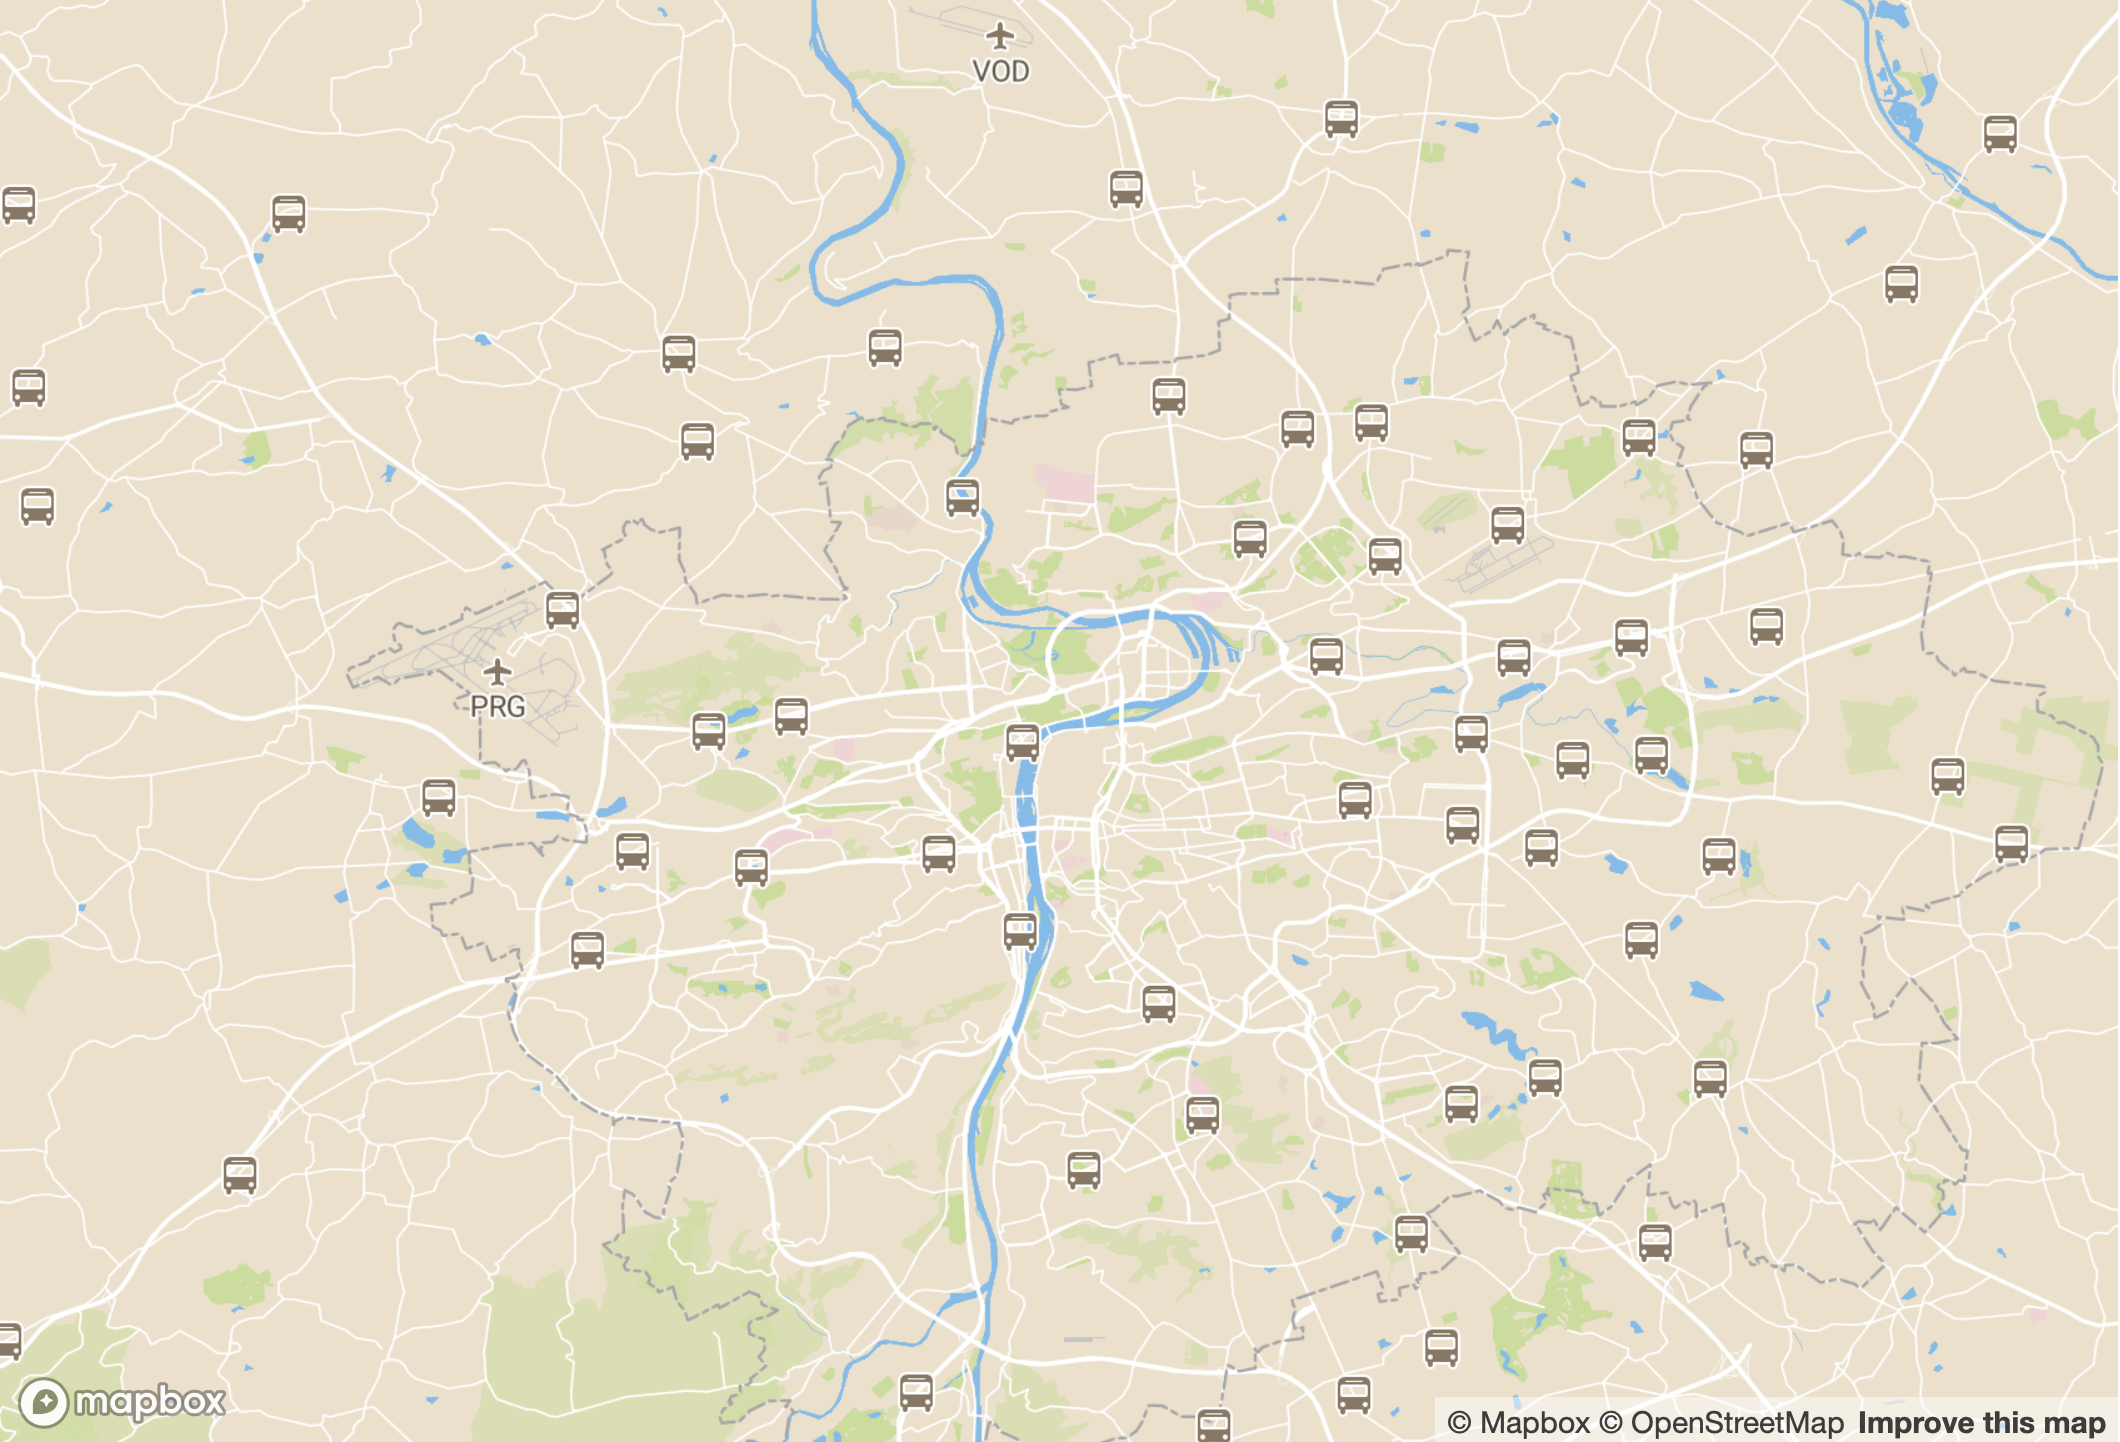
\includegraphics[width=\linewidth]{../img/golemio_mapa.png}
  \caption{Mapa z golemio.cz.}
  \label{fig:golemio_result}
\end{figure}

\subsubsection{Tram-bus}

Dalším poskytovatelem je portál tram-bus, který si vede o něco lépe. Ukazuje směr jízdy vozidel, čísla linek a po kliknutí informace o zpoždění a nejbližší zastávky. Pozn.: na mapě již jsou vidět spoje \gls{dpp}, protože v době psaní této práce již byly data veřejné.

\begin{figure}
  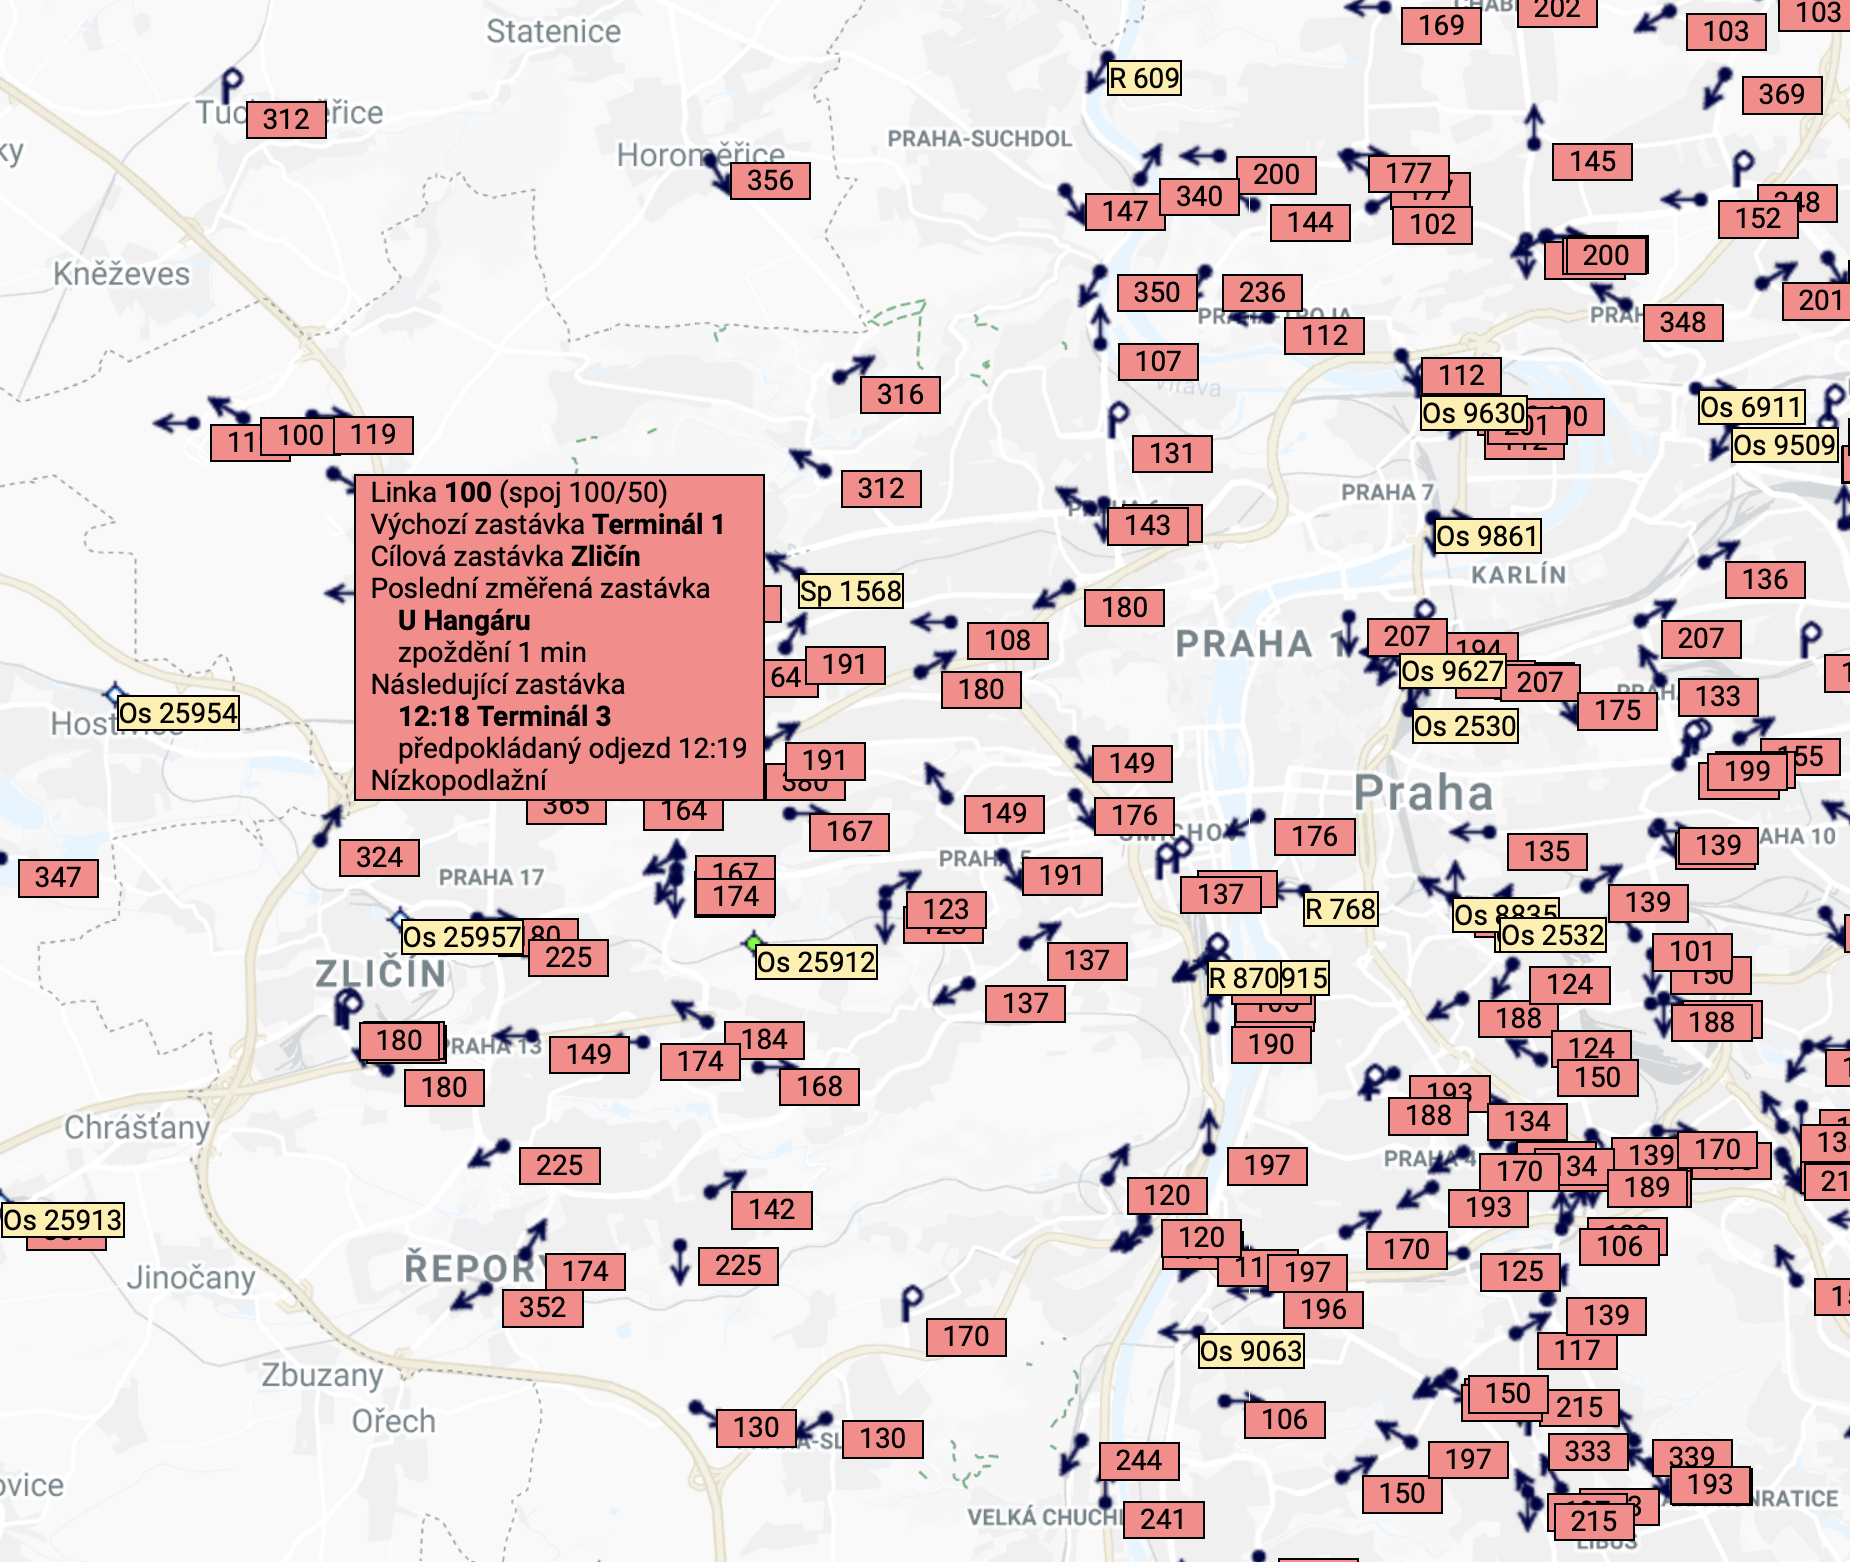
\includegraphics[width=\linewidth]{../img/tram-bus_mapa.png}
  \caption{Mapa z www.tram-bus.cz.}
  \label{fig:tram-bus_result}
\end{figure}

\subsubsection{\gls{idsjmk}}

Mimo Prahu je velice pěkně udělaná aplikace pro zobrazení vozidel \gls{idsjmk} (Integrovaný dopravní systém Jihomoravského kraje). Ten ihned po načtení stránky zobrazuje všechny dobravní prostředky, tedy tramvaje, autobusy a vlaky vše s čísly linek. Dále pak umožňuje po kliknutí na vybraný spoj zobrazit více informací včetně jízdního řádu.

\bigbreak

Tato aplikace je po vizuální i funkční stránce dobrou inspirací pro tvorbu aplikace v této práci.

\begin{figure}
  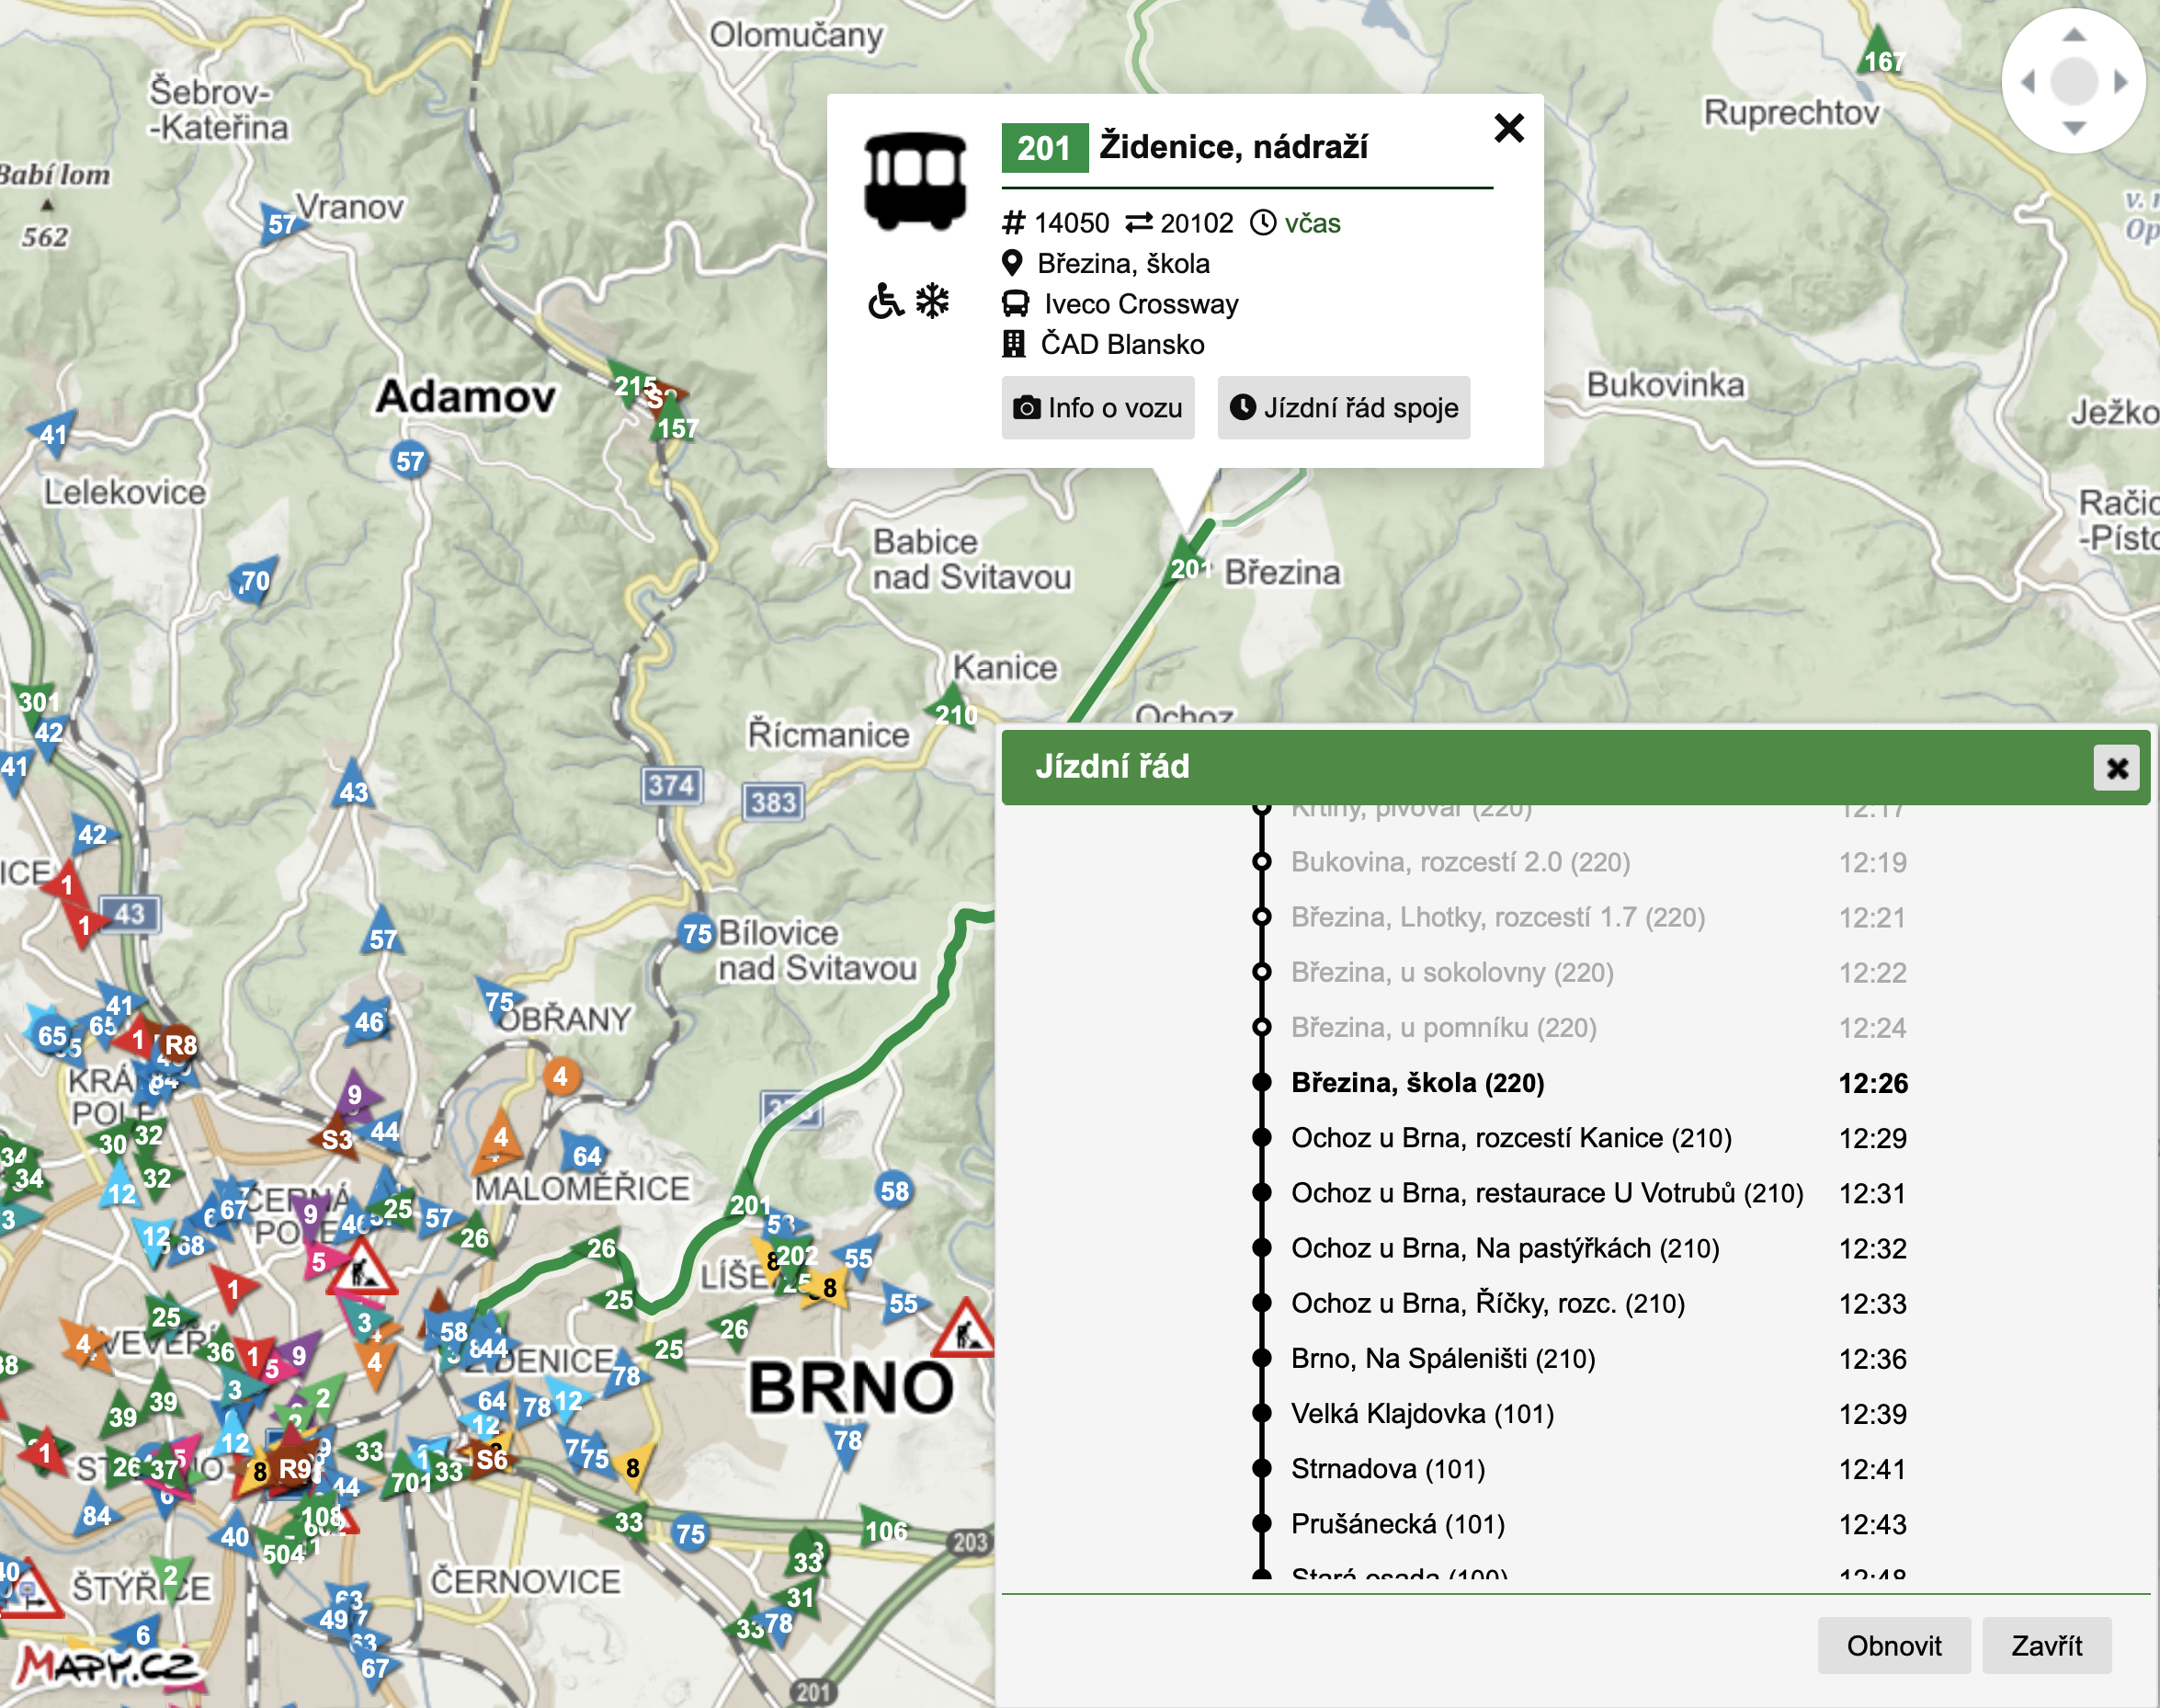
\includegraphics[width=\linewidth]{../img/idsjmk_mapa.png}
  \caption{Mapa z mapa.idsjmk.cz.}
  \label{fig:idsjmk_result}
\end{figure}

%%% Fiktivní kapitola s ukázkami sazby

\chapter{Návrh řešení}

V této kapitole je popsán návrh technického řešení uvedených problémů.

\section{Úvod}

Běh celé aplikace bude rozdělen do dvou částí.

\begin{itemize}
	\item Stahování a ukládání real-time dat o polohách vozidel do datového skladu, které budou doplněny o odhat zpoždění pro okamžité zveřejnění v uživatelské aplikaci.

	\item Modelování profilů jízd jednotlivých úseků. Tyto modely budou pak dále sloužit k odhadování zpoždění v budoucnu.  Výpočet modelů bude prováděn jednou za delší časový úsek (nejlépe jednou za den).
\end{itemize}

Protože obě části jsou na sobě závislé v iniciálním běhu bude prováděna první část sběru dat bez odhadu zpoždění, nebo pomocí již existujícího triviálního lineárního odhadu.

\bigbreak

Schéma návrhu celé aplikace a komunikační mapa jednotlivých komponent je ilusrtována na diagramu \ref{fig:design_diagram}.

\begin{figure}
	\centering
  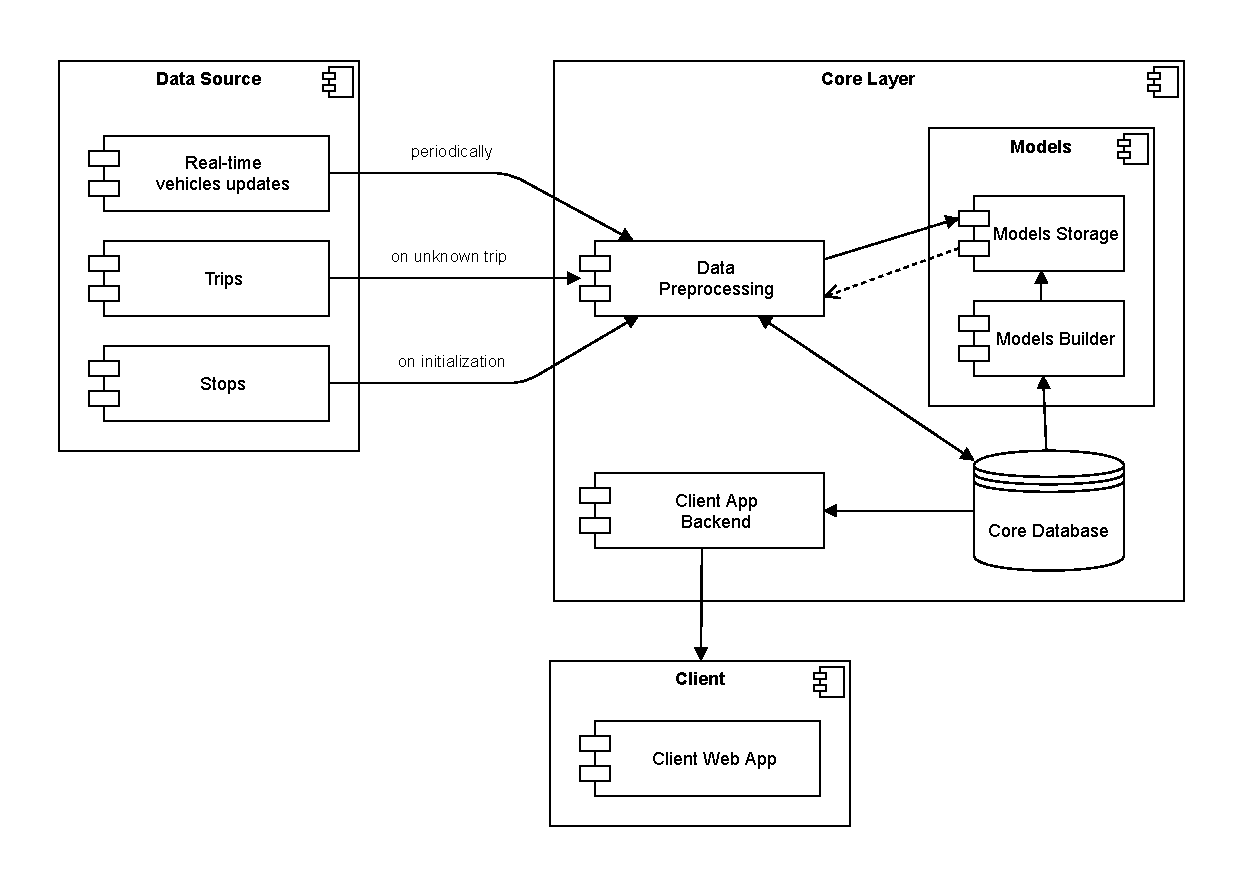
\includegraphics[width=140]{../img/design_diagram}
  \caption{UML diagram návrhu aplikace}
  \label{fig:design_diagram}
\end{figure}

\subsection{Funkční a kvalitativní požadavky}

Nejprve specifikujme požadavky systému, na kterém se pak bude zakládat
konkrétní návrh řešení backendu celé aplikace (bez vizualizace).

\subsubsection{Funkční požadavky}

\begin{itemize}
	\item
Popsaný odhad změny zpoždění na trase mezi dvěma referenčními body je nutné počítat v co nejkratším čase tak, aby cestující byli dobře informování o stavu jejich spoje a mohli tyto informace využít např. při dobíhání spoje. A proto je potřeba zpracovávat data okamžitě po jejich vydání, spočítat odhad zpoždění a vystavit tato data veřejně. Vzhledem k tomu, že tato data velmi rychle zastarávají je nutné provádět tento proces co možná nejrychleji\footnote{Průměrná doba jízdy spoje mezi zastávkami je cca 5 min. Rozložení počtu úseků mezi zastávekami k délce jízdy mezi nimi je závislé a podobné rozložení vůči vzdálenosti ilustrované na grafu\ref{fig:stop_distances_result}.}.

\item

Data o polohách vozidel VHD v Datové platfomě jsou aktualizována nejpozději každých 20 sekund, více v kapitole \ref{chapter:analyza_zdroje}. Tedy pro minimalizaci rychlosti zastarávání dat a získání všech existujících vzorků dat o polohách je nutné data stahovat alesponˇ každých 20 sekund.

\item

Odhad zpoždění se bude provádět na základě historických dat z posledních vyšších jednotek dnů\footnote{Pro demonstrativní účely této práce jsou využívány historická data pouze ze 4 dnů (2 pracovní a 2 víkendové).}. Tím se sníží dopad mimořádné události na předpovědní model, která může na trase vzniknout. Zárovenˇ by však neměla být započítávána data starší několik týdnů, protože dopravní situace se mění v závislosti na ročním období nebo také pokud je na trase delší omezení dopravy je požadováno, aby se takové omezení projevilo co možná nejdříve. Navíc se bude rozlišovat mezi daty z pracovních dnů a nepracovních dnů, to protože samotné jízdní řády se mohou lišit (doba jízdy mezi mezastávkama) a také se do velké míry liší hustota dopravy, která ma velký vliv na profil jízdy. TODO do navrhy na zlepseni: Pro zpřesnění výsledků by bylo lepsi respektovat svatky, kazdy den v tydnu zvlast atp.

\item

Zpracování historických dat bude probíhat vždy po delší době, nejlépe jednou za den. To umožní provádět náročnější výpočty, které by za normálního provozu neúměrně přetížily systém. Navíc vzhledem k povaze cíle práce ani není žádoucí zpracování historických dat provádět častěji než jednou denně, protože se nepokoušíme okamžitě reagovat na změnu dopravní situace.

\item

Uložená historická data budou struktorovaná tak, aby nad nimi šly provádět statistické výpočty minimálně o frekvencích spojů, vzdálenostech tras, zpoždění spojů.
\end{itemize}

\subsubsection{Kvalitativní požadavky}

\begin{itemize}

	\item
	Řešení bude schopno při jedné aktualizaci zpracovat alesponˇ 1000\footnote{20. 2. 2020 mezi 7:00 a 7:10 bylo na trase přes 600 vozidel} vzorků poloh vozidel, kde 10 \% vzorků může být o dosut neznámých jízdách. V tomto případě je potřeba stáhnout jízdní řád konkrátní jízdy a její jízdní profil, což navíc dotaz na zdroj dat.

	\item
	Vypočítané modely profilů jízd budou dávat odhat zpoždění lepší, než je lineární odhad. To znamená, že zpoždění vypočítaná pro každý přijatý vzorek polohy vozidla mezi dvěma referenčními body na trase bude mít menší rozptyl než lineární odhad zpoždění.

\end{itemize}


\section{Zpracování vstupních dat}

Struktura uložení dat se zakládá na struktuře zdrojových dat popsaných v kapitole \ref{section:analyza_zdroje} Analýza zdroje dat.

\bigbreak

Na datové platformě jsou real-time data o vozidlech dostupná do historie řádově jednotek minut, což je naprosto nedostatečné pro jakékoliv pozdější využití v ránci této práce. Především pro počítání statistik a modelování profilů jízd nad daty je potřeba zřídit lokální databázi, která bude držet historická data tak, jak byla obdržena od zdroje. Navíc data jsou poskytována ve formátu \gls{json}, který svou povahou není zrovna úsporný co se do velikosti souboru týče. Proto je vhodné zvolit ukládání dat v jiném formátu.

\subsection{Databáze}

Za tímto účelem tato práce využívá relační databázi obsluhovanou dotazovacím jazykem \gls{sql}. Struktura databáze je vyobrazena na EER diagramu \ref{obr:EER}\footnote{SQL dotazy na sestavení celé databaze jsou definovány v příloze database.sql. Pro testovací, debugovací a demonstrační účely slouží navíc i jiné databáze, které jsou struktorou totožné jako produkční databáze.}. Tato databáze se skládá z 5 tabulek. Jsou jimi:


\begin{figure}[p]\centering
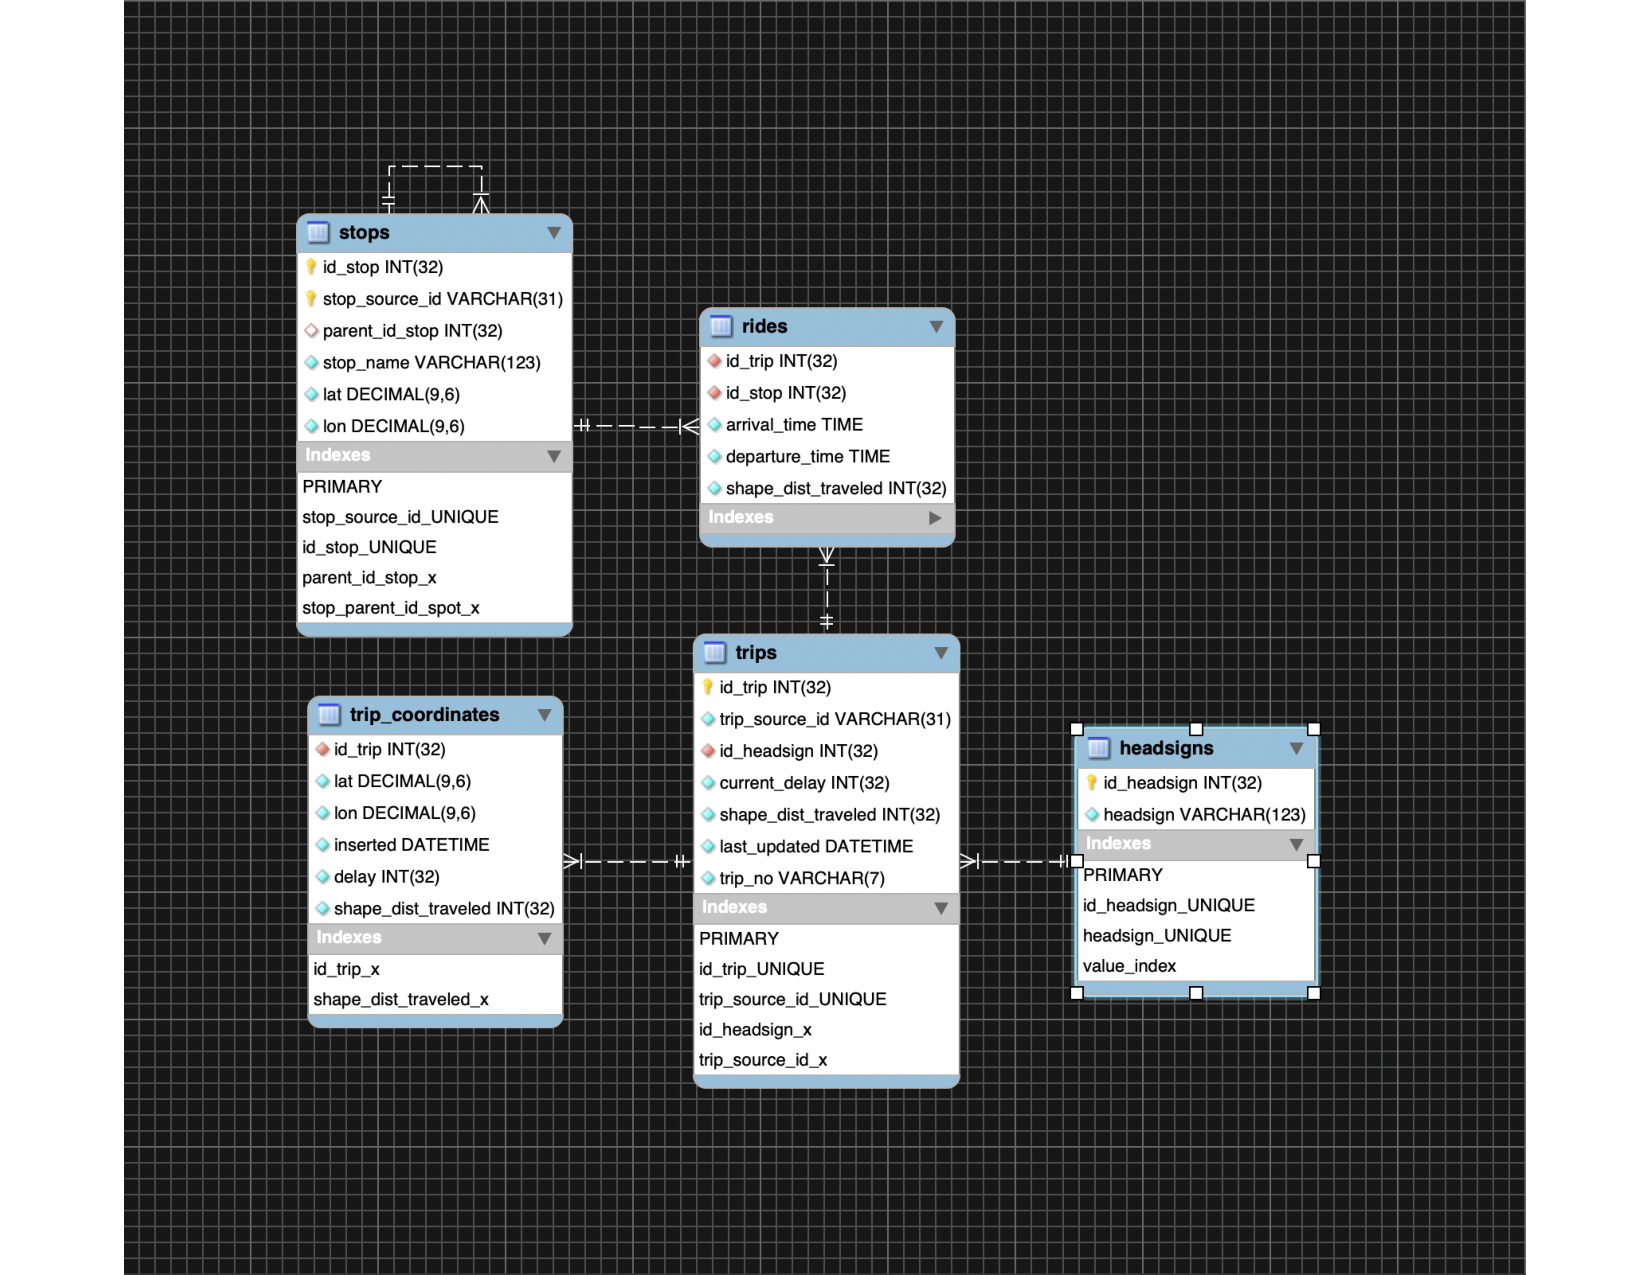
\includegraphics[width=140mm]{../img/eer_database}
% Příponu není potřeba explicitně uvádět, pdflatex automaticky hledá pdf.
% Rozměry také není nutné uvádět.
\caption{EER diagram databáze.}
\label{obr:EER}

\end{figure}

\begin{itemize}
	\item \verb-trips- všechny objevené jízdy

		\begin{itemize}
			\item \verb-id_trip- unikátní identifikátor používaný v databázi

			\item \verb-trip_source_id- identifikátor tripu převzatý ze zdroje dat

			\item \verb-id_headsign- identifikátor nápisu pro daný trip

			\item \verb-current_delay- aktuální zpoždění tripu

			\item \verb-shape_dist_traveled- aktuální vzdálenost ujetá od výchozí stanice

			\item \verb-last_updated- čas poslední aktualizace, převzatý ze zdroje dat

			\item \verb-trip_no- číslo dané linky
		\end{itemize}

	\item \verb-headsigns- nápisy nad vozidlem, cílová stanice

		\begin{itemize}
			\item \verb-id_headsign- unikátní identifikátor nápisu

			\item \verb-headsign- text nápisu
		\end{itemize}

	\item \verb-trip_coordinates- všechna historická real-time data

		\begin{itemize}
			\item \verb-id_trip- identifikátor tripu, ke kterému se záznam váže

			\item \verb-lat- zeměpisná šířka polohy vozidla

			\item \verb-lon- zeměpisná délka polohy vozidla

			\item \verb-inserted- čas vložení záznamu

			\item \verb-delay- zpoždění zachycené v poslední projeté stanici před pořízením záznamu

			\item \verb-shape_dist_traveled- vzdálenost ujetá od výchozí stanice tripu

		\end{itemize}

	\item \verb-stops- všechny zastávky

		\begin{itemize}
			\item \verb-id_stop- unikátní identifikátor zastávky

			\item \verb-trip_source_id- identifikátor zastávky převzatý ze zdroje dat

			\item \verb-parent_id_stop- identifikátor rodičovské zastávky, pokud existuje

			\item \verb-stop_name- název zastávky

			\item \verb-lat- zeměpisná šířka polohy zastávky

			\item \verb-lon- zeměpisná délka polohy zastávky

		\end{itemize}

	\item \verb-rides- trasa každého tripu, seznam zastávek s časy odjezdů a příjezd tvořící jízdní řád

	\begin{itemize}
		\item \verb-id_stop- identifikátor tripu

		\item \verb-id_stop- identifikátor zastávky

		\item \verb-arrival_time- čas příjezdu tripu do zastávky

		\item \verb-departure_time- časodjezduu tripu ze zastávky

		\item \verb-shape_dist_traveled- vzdálenost zastávky od výchozí zastávky tripu

	\end{itemize}

\end{itemize}

Atributy se jménem *source\_id jsou pravděpodobně unikátní identifikátor entity ve zdroji dat, nicméně z dokumentace zdroje to nevyplývá. Také je tento indenfikátor ukládán jako textový řetězec, ačkoli je tvořen pouze číslicemi a podtržítky, není nikde zaručeno, že jej lze jednoduše převést na číselný ko'd. Takže pro lepší výkon databáze je použito automaticky generované id typu \gls{int}.

\bigbreak

Každá tabulka má několik indexů, které zlepšují výkon databáze při vkládání a hledání dat. Obvzláště pokud je atribut označen jako unikátní, kde se při každém vložení ověřuje unikátnost.

\bigbreak

Databáza je nastavená tak, aby umožňovala získat všechny potřebné informace o vozidlech, ale hlavně přístup k historickým real-time datům a to separovaně pro dvojci refenčních bodů.

\subsection{Plnění databáze}

Tato databáze bude plněna skriptem, jehož bude naprogramován taky, aby vždy stáhl aktuální obraz dopravní situace a tato data uložil do dotabáze. Toto stahování z datové platformy probíhá podle násldujícího algoritmu.

\bigbreak

Algoritmus:
\begin{code}[frame=none]
načti všechny dostupné zastávky
dokud skrip běží
  načti aktuální polohy vozidel
  pro každé nalezené vozidlo
  pokud jízda vozidla je známá
    aktualizuj data o jízdě
  jinak
    stáhni informace o jízdě
    zpracuj a vlož jízdu do databáze
\end{code}

\bigbreak

Protože všechny infomace ukládané do databáze jsou důležité pro hlavní cíl této práce, tak pokud se vyskytne jízda, který neobsahuje některou z požadovaných infomarcí je pak automaticky zahozena. To je řešeno pomocí databázových transakcí tak, aby stav databáze byl vždy konzistentní. Transakce v obecném smyslu fungují tak, že můžeme měnit data v databázi (i více zázanamů) a tyto změny se zapíší do samotné databáze až po potvrzení, že všechny změny byly provedeny správně, pokud během provádění změn nastane chyba, můžeme v jakékoli fázi provádění změn všechny dosud proveedné změny zahodit a vrátit se do původního stavu databáze před započetím transakce.  Tedy pokud nejsou poskytnuta data ve formátu, který skript akceptuje, nebo nějaké povinné atributy chybí. Vložení celé jízdy nebude provedeno.

\bigbreak

Nejčastěji chybějící atribut je zpoždění v poslední zastávce, toto je nutné vědět pro počítání zpoždění mezi refenrečními body (zastávkami). Absence této informace může být způsobena tím, že vozidlo vůbec nevysílá data potřebnák k jejím dopočtení, pak nemá smysl jej do databáze zahrnovat. Nebo vozidlo už vysílá, ale ještě nezahájilo jízdu, tedy nemá žádnou poslední projetou zastávku, v takovém případe budou data ignorována až do doby příchodu první relevantní informace.

\bigbreak

Mimo popsanou databázi se do určeného adresáře ukládají trasy jednotlivých jízd, která jsou ve fromátu \gls{geojson} jako lomená čára definována souřadnicemi. Navíc data o trasách jsou používána pouze pro vizualizaci a jsou přijímány vizualizačním nástrojem ve formátu \gls{geojson}, tedy tyto data není nutné vůbec transformovat a není nutné je držet v hlavní databázi.

\bigbreak

 Stejně tak i aktuální polohy vozidel jsou mimo databázi zapisovány do souboru, který je určen a formátován pro čtení webovou aplikací. Aktualizace tohoto souboru je provedena přednostně, ihned po načtení real-timových dat. Tím se zabrání nechtěnému čekaní na aktualizaci celé databáze, která může trvat jednotky sekund.


\section{Algoritmus odhadu zpoždění}



\section{Vizualizace dat}

\subsection{Funkční požadavky}

\begin{itemize}
	\item

	\item Aplikace vykreslí interaktivní mapu Prahy a širšího okolí, kterou bude možné posouvat či zoomovat. V této mapě budou zobrazeny vozidla na aktuálních pozicích a budou se automaticky posouvat po mapě, tak jak se pohybují ve skutečnosti.

	\item Po kliknutí na vozidlo se zobrazí jeho celá trasa včetně zastávek a jeho dopočítaného zpoždění.

	\item Po kliknutí na zastávku se zobrazí seznam spojů, které budou projíždět vybranou zastávkou a jejich trasy se vykreslí do mapy.

	\item Celá aplikace bude postavena na principu server -- client. Tedy serverová strana se postará o přístup k otevřeným datům o vozidlech a jejich uložení a také obsluhu požadavků klienta. Klientská část bude webová stránka poskytující služby popsané výše. Měla by být schopná zobrazit řádově tisíce vozidel.
\end{itemize}

\subsubsection{Nefunkční požadavky}

\begin{itemize}
	\item Serverová část bude napsaná v jazyce Python 3.

	\item Webová část bude napsaná pomocí jazyků pro webové technologie, převážně v JavaScriptu.

	\item Pro vykleslení mapy bude využita služba Mapbox.

	\item Ukládání dat na serverové straně bude řešeno MySQL databází.

	\item Pro algoritmus odhadu zpoždění na zákldě historických dat budou využity různé knihovny pro jazyk Python 3. Zejména pak scikit-learn a alphashape.

\end{itemize}

\subsubsection{Proces běhu aplikace}

Jak je již zmíněno aplikace bude využívat historická data, tedy bude nutné nechat aplikaci tato data nějakou dobu sbírat. Pro efektivní odhady by bylo vhodné mít uložené historické polohy vozidel alespoň z uplynulých několika týdnů.

\bigbreak

Avšak již v průběhu sběru dat může aplikace poskytovat základní službu a to vizualizování vozidel v mapě.

\subsection{Poskytovatelé mapových podkladů}

K takovému účelu nejlépe poslouží vykreslení aktuálních poloh vozidel do mapy, kde se po vyžádání uživatelem tyto data zobrazí.

\bigbreak

Za účelem vytvoření dostatečně přívětivé uživatelské aplikace je nezbytné využít některého z poskytovatelů mapových podkladů a zanést do něj získané informace.

\bigbreak

Jedním z těchto poskytovatelů je společnost Google, která má propracované mapové podklady a prostřednictvím služby Google Maps poskytuje pro tuto práci požadovanou službu. Další platformou je Mapbox, který poskytuje velmi podobné služby jako Google Maps. Nicméně narozdíl od Googlu využívá jako mapový podklad \gls{osm} {otevřená geografické data}. Protože smyslem práce je v co největší míře využít otevřená data je žádoucí využít právě Mapbox.

\bigbreak

TODO dokumentace mapbox, zeptat se jestli je to vubec nutne rozebirat

%%% Fiktivní kapitola s ukázkami tabulek, obrázků a kódu

\chapter{Implementace}

V této kapitole je detailně popsána implementace a volba technologií použití k implementaci navrženého díla.

\section{Úvod}

Nejdůležitější částí celého systému je modul výpočtu a používání pravděpodobnostních modelů odhadu zpoždění vozidel. To vytváří požadavek na využití technologií, které poskytují prostředí pro pohodlnou tvorbu těchto modelů. V současnosti jsou nejpokročilejší nástroje pro takový účel součástí balíčkové sady jakyka Python3, konkrétně se jedná o knihovnu scikit-learn\footnote{https://scikit-learn.org/stable/} a další nástroje pro páci s velkými daty jake je knihovna NumPy\footnote{https://numpy.org}. Tyto knihovny implemntují dobře známé algoritmy umělé inteligence, včetně optimalizací a pomocných funkcí zjednodušujících hledání nejlepšího modelu. Navíc jsou tyto knihovny naimplementovány s ohledem na vysokou výkonost\footnote{https://scikit-learn.org/stable/developers/performance.html} a využití grafických karet\footnote{Záleží na konkrétním hardwaru}. Proto nedává smysl jejich služeb nevyužít. Využití jazyka Python3 je tedy pro jádro náší práce jasnou volbou.

\bigbreak

Pro samotné zpracování dat žádné speciální požadavky nevyvstávají a je možné využít i jiné ověřené backendové programovací jazyky a technologie. Nicméně pro zachování jednoty vývoje není důvod měnit prostředí a využijeme též jazyk Python3. Může být namítnuto, že programy psané v jazyce Python3 nejsou výkonostně příliš dobré, nicméně v našem případě se nebudou provádět žádné složité výpočty, ale pouze stahování dat z internetu a jejich transformace. Bytˇ se jedná o poměrně velké objemy dat jakákoliv operace s nimi je stále řádově rychlejší než stahování z internetu.

\bigbreak

Databázi jsem již vybrali MySQL\footnote{https://www.mysql.com} implementaci. To zejména z důvodů, že se jedná o open source projekt a tato implementace je velmi často vyžívaná v celé řadě jiných projektů s velkou komunitou. Konkrétně pro Python3 existuje knihovna MySQL Connector\footnote{https://dev.mysql.com/doc/connector-python/en/} přes kterou je možné \gls{sql} databázi pohodlně obsluhovat.

\bigbreak

Celý systém je ovládaný přes hlavní skript v souboru \verb-download_and_process.py-. Tento skript slouží jak ke spuštění produkčního běhu aplikace tak i k údržbě dat, správným nastavení parametrů se vybere zdroj dat, kde je navýběr mezi demonstračními daty, vývojovými daty nebo real-time dady. Dále je možné spuštěním skriptu vytvořit modelu profilů jízd a táké odstranit historická data z databáze podle jejich data vložení.

\bigbreak

Veškerý software bude naimplemtván s ohledem na paradigma \gls{oop}. Tedy logické celky budeme dělit do tříd, jejichž instance budou repzentovat vždy danou entitu. Každá třída bude implemenovat sadu metod, odpovídající logice věci.

\section{Zpracování dat} \label{section:zpracovani_dat}

Základní myšlenka zpracování dat pocházejících ze zdroje dat popsaném v kapitole \ref{section:analyza_zdroje} je taková, že data se budou periodicky stahovat a ukládat do \gls{sql} databáze, tento postup je popsán v kapitole \ref{section:zpracovani_vstupnich_dat}.

\bigbreak

Jako součást projektu naimplementujeme pro přehlednost pomocné třídy celkově usnadnˇující využití zdrojů a technologií pro náš specifický účel. Dále pak z důvodu oddělení technických záležitostí, jako je např.: stahování dat ze sítě, tak aby nezasahovali do ko'du implementující logiku systému. Stejně tak se tímto eliminuje výskyt paternů v celém ko'du. Konktrétně se tím myslí komunikace s databází, kominkace se zdrojem dat, komunikace se souborovým systémem. Tyto třídy navíc definují důležité konstanty, jakými jsou např.: jména využívaných souborů nebo souborových adresářů, \gls{url} zdroje dat atp.

\bigbreak

Hlavní smyčka ve které se stahují a zpracovávají data volá následující funkce.

\begin{code}[frame=none]
# stažení aktuálních poloh vozidel
all_vehicle_positions.get_all_vehicle_positions_json()

# konstrukce interní reprezentace vozidel
all_vehicle_positions.construct_all_trips(database_connection)

# odhadnutí spoždění všech vozidel
estimate_delays(all_vehicle_positions, models)

# kompletace dat a uložení do databáze
asyncio.run(process_async_vehicles(all_vehicle_positions, database_connection, args))
\end{code}

\subsection{Konstrukce objektů vozidel}

Funkce \verb-construct_all_trips- vytvoří z každého nalezeného vozidla ve vstupním \gls{json} souboru instanci třídy \verb-Trip-, která je interní reprezentací těchto vozidel.

\bigbreak

Avšak ke konstrukci instancí vozidel je potřeba získat data z databáze o jízdních řádech. To potože součástí vstupního souboru z externího zdroje není informace o poslední projeté a další následující zastávce. Tuto informaci potřebujeme pro odhad zpoždění provádějící se v dalším kroku\footnote{Ve verzi 2 datového formátu souboru poloh vozidel je již tato informace zahrnuta}. Proto se na začátku konstrukce instancí třídy \verb-Trip- čtou data z tabulky \verb-rides- pouze pro aktuálně zpracovávané jízdy, a dále se pak sadou funkcí hledá poslední projetá a následující zastávka na trase každého spoje.

\subsection{Odhad zpoždění}

Tato funkce odhadu zpoždění musí být volána ještě před uložením do databáze, aby se do databáze vložily data včetně odhadu zpoždění. To ovšem zapříčiní, že pokud je vozidlo dosud nenalezeno neznáme ani jeho jízdní řád a tedy nemůžeme pro něj odhadnou zpoždění. To ovšem nehraje velkou roli, protože se tak stane pro každé vozidlo ihned po vyjetí z výchozí stanice, nebo ještě pře vyjetím, v těchto případech nemá počítání odhadu zpoždění velký význam. V další iteraci již jízdní řády spoje budou známé, tedy chybějící zpoždění doplníme velmi rychle.

\bigbreak

Funkce odhad zpoždění využívá zkonstruovaných modelů profilů jízd, pokud takový model zatím není vytvořen použije se zpoždění v poslední projeté zastávce. Modely jsou uloženy v souborovém systému a pro každou dvojci zastávek je model uložen zvláštˇ.

\bigbreak

Pro rychlejší běh aplikace jsou však po prvním načtení modely drženy v paměti počítače v proměnné typu mapa, to nám pak umožní rychlé vyhledávání podle dvojce identifikátorů zastávek. Implementace funkce je následující, tento ko'd je volán pro každé vozidlo zvláštˇ.

\begin{code}[frame=none]
# najde model podle dvojce zastávek a dnů v týdnu
model = models.get(
  str(vehicle.last_stop or '') + "_" +
  str(vehicle.next_stop or '') +
  ("_bss" if lib.is_business_day(vehicle.last_updated) else "_hol"),
  Two_stops_model.Linear_model(vehicle.stop_dist_diff))

# vybere data potřebná k výpočtu odhadu zpoždění
tuple_for_predict = vehicle.get_tuple_for_predict()

# odhadne zpoždění
# jinak se při vkládání do databáze použije zpoždění z poslední zastávky
if tuple_for_predict is not None:
  vehicle.cur_delay = model.predict(*tuple_for_predict)
\end{code}

\subsection{Kompletace dat a jejich uložení}

Kompletace dat především obnáší stažení dalších dat, jako jsou jízdní řády v případě, že jízda doposud nebyla nalezena. Takových jízd může být v jedné iteraci běžící aplikace i několik desítek, při spuštění systému jsou všechny jízdy nenalezeny a tedy musí být staženy dodatečná data i pro několik stovek jízd. Aby se data o každé jízdě nestahovala sériově metoda zpracování vozidel je implementována asynchroně, resp. stahování dat je asynchroní. Díky tomu se začnou stahovat data o více jízdách v jeden okamžik. Bytˇ čekání na stažení dat o jedné jízdě je při dobrém internetovém spojení otázkou několika desítek milisekund, tak v případech stahování dat o stovkách jízd sériově by jenom stahování dat prodloužilo běh jedné iterace o jednotky až nízké desítky sekund.

\bigbreak

Jak tedy vyplývá z textu výše tato funkce dělí běh na dvě části podle toho jestli je jízda vozidla nalezena nebo nenalezena. V případě nalezené jízdy v databázi se jen aktualizuje záznam v tabulce \verb-trips-, mezi aktualizovaná data patří aktuální zpoždění, zpoždění v poslení pojeté zastávce, ujetá vzdálenost, souřadnice vozidla a časová známka aktualizace dat ve zdroji dat. Zárovenˇ s aktualizací dat v tabulce \verb-trips- se provádí i vložení nového záznamu do tabulky \verb-trip_coordinates-, která slouží jako datový sklad všech zaznamenaných poloh vozidel. Celá logika aktualizace je řešena v \gls{sql} funkci.

\begin{code}[frame=none]
CREATE DEFINER=`root`@`localhost` FUNCTION
  `update_trip_and_insert_coordinates_if_changed`(
  trip_source_id_to_insert VARCHAR(31),
  current_delay_to_insert INT(32),
    last_stop_delay_to_insert INT(32),
  shape_dist_traveled_to_insert INT(32),
  lat_to_insert DECIMAL(9,6),
  lon_to_insert DECIMAL(9,6),
  last_updated_to_insert DATETIME) RETURNS int(1)
    DETERMINISTIC
BEGIN
  SELECT last_updated, id_trip
  INTO @last_updated, @id_trip
  FROM trips
  WHERE trips.trip_source_id = trip_source_id_to_insert
  LIMIT 1;

  IF @last_updated <> last_updated_to_insert THEN
    INSERT INTO trip_coordinates (
      id_trip,
      lat,
      lon,
      inserted,
      delay,
      shape_dist_traveled,
      last_stop_delay)
    VALUES (
      @id_trip,
      lat_to_insert,
      lon_to_insert,
      last_updated_to_insert,
      current_delay_to_insert,
      shape_dist_traveled_to_insert,
      last_stop_delay_to_insert);

    UPDATE trips
    SET trips.last_updated = last_updated_to_insert,
      trips.current_delay = current_delay_to_insert,
      trips.shape_dist_traveled = shape_dist_traveled_to_insert,
      trips.lat = lat_to_insert,
      trips.lon = lon_to_insert
    WHERE trips.id_trip = @id_trip;
        RETURN 1;
  ELSE
    RETURN 0;
  END IF;
END
\end{code}


\section{Konstrukce modelů}


Pro spočítání polynomiálního modelu se využívá knihovna sklearn konkrétně algoritmus zvaný Rigde, který sám o sobě hledá linární závislosti, nicméně vstupní hodnoty jsou mezi sebou náležitě pronásobeny tak, aby simulovali polynomiální funkci. Toho se dosáhne pomocí funkce PolynomialFeatures. Optimální stupeň polynomu se zjistí spočítáním modelu pro každý stupeň v rozumných mezích a nakonec se zvolí ten s nejmenší chybou. To se v jazyce Python3 za pomocí knihovny sklearn provede následujcícm ko'dem. Omezení stupnˇů polynomiální regrese vyplývá ze skušenosti, kdy s nejmenší chybou jsou modely stupně 5 nebo 6.

\begin{code}[frame=none]
for degree in [3, 4, 5, 6, 7, 8, 9, 10]:
  model = make_pipeline(PolynomialFeatures(degree), Ridge(), verbose=0)
  model.fit(X_train, y_train)
  pred = model.predict(X_test)
  error = mean_squared_error(y_test, pred)
  if error < best_error:
    best_degree = degree
    best_error = error

self.model = make_pipeline(PolynomialFeatures(best_degree), Ridge())
self.model.fit(input_data, output_data)
\end{code}

Samotné nalezení správného modelu se nyní může zdát jednoduché, nicméně nejsložitější prací pro jakoukoli úlohy z oblasti umělé inteligence a strojového učení je příprava dat a v naší práci tomu není jinak. Atˇ už se jedná o samotná zpracování dat popsané výše v kapitole \ref{section:zpracovani_dat}, tak také je potřeba tyto zpracovaná data dále trasnformovat z formátu v jakém jsou uloženy v databázi do formátu jaký je vhodný pro počítání lineární regrese. Dále je pak potřeba data vyčistit od zcela nesmyslných vzorků poloh vozidel, kterých je vstupních datech spousta a mohly by negativně ovlivnit správnost odhadů nalezených modeů.

\subsection{Čtení dat}

Pro zkonstuování modelů popisujících profily jízd mezi všemi dvojcemi zastávek je nejprve potřeba zjistit všechny dvojce zastávek, mezi kterými jede alesponˇ jeden spoj. To se dá zjistit pomocí jízdních řádů, které reprezentujeme v tabulce \verb-rides- v naší databázi popsané v kapitole \ref{subsection:databaze}

\bigbreak

 Dále pokud máme všechny dvojce zastávek je potřeba získat všechny oznámené polohy vozidel mezi nimi pro každou dvojci zastávek zvláštˇ. To je možné realizovat pomocí následujícího \gls{sql} dotazu.

\begin{code}[frame=none]
SELECT schedule.id_trip,
  schedule.id_stop,
  schedule.lead_stop,
  departure_time,
  schedule.lead_stop_departure_time,
  (schedule.lead_stop_shape_dist_traveled - schedule.shape_dist_traveled)
    AS diff_shape_trav,
  trip_coordinates.inserted,
  (trip_coordinates.shape_dist_traveled - schedule.shape_dist_traveled)
    AS shifted_shape_trav,
  trip_coordinates.delay
FROM (
  SELECT id_trip, id_stop, shape_dist_traveled, departure_time,
    LEAD(id_stop, 1) OVER (PARTITION BY
	  id_trip ORDER BY shape_dist_traveled) lead_stop,
    LEAD(shape_dist_traveled, 1) OVER (PARTITION BY
	  id_trip ORDER BY shape_dist_traveled) lead_stop_shape_dist_traveled,
    LEAD(departure_time, 1) OVER (PARTITION BY
	  id_trip ORDER BY shape_dist_traveled) lead_stop_departure_time
  FROM rides) AS schedule
JOIN trip_coordinates
ON trip_coordinates.id_trip = schedule.id_trip AND
  schedule.lead_stop_shape_dist_traveled -
    schedule.shape_dist_traveled > 1500 AND
  trip_coordinates.shape_dist_traveled
    BETWEEN schedule.shape_dist_traveled AND
  schedule.lead_stop_shape_dist_traveled
ORDER BY id_stop, lead_stop, shifted_shape_trav
\end{code}

Tento SQL dotaz nejprve získá všechny dvojce po sobě jdoucích zastávek z jízdních řádů v tabulce \verb-rides-. Protože v tabulce je jízda spoje uložená jako sekvence zastávek, kde každé náleží čas příjezdu resp. odjezdu a její vzdálenost na trase spoje od výchozí stanice spoje (atribut \verb-shape_dist_traveled-). Tedy dvojce zastávek po sobě následující se získají tak, že se seřadí všechny zastávky pro každý spoj podle atributu \verb-shape_dist_traveled-. Následující zastávka pak je ta ležící na následujícím řádku v seřazené tabulce, tento řádek se přečte pomocí funkce \verb-LEAD-.

\bigbreak

K těmto dvojcím zastávek dále získáme všechny vzorky poloh vozidel. To tak, že vezme všechny vzorky pro daný spoj, které leží mezi vybranou dvojcí zastávek. V tomto dotazu zárovenˇ vyloučíme zastávky, které jsou k sobě blíže než nebo vzdálené přesně 1500 m (v implementaci je pak vzdálenost určena parametricky), zdůvodnění této vzdálenosti je výše v návrhu modelů. Pro produkční nasazení je ještě potřeba omezit čtené vzroky podle času vytvoření, tedy např. nevyužívat vzorky starší několika dní, jak je popsáno v analýze problému. Nicméně toto omezení by vycházelo z reálného provozu ze skušeností jak rychle se vývíjí dopravní sítˇ nebo jak často se mění jízdní řády.

\bigbreak

Takto jak je SQL dotaz napsán, je jeho provedení velmi časově náročné. To nám, ale nemusí vadit protože dotaz bude volán pouze před výpočtem modelů, což je samo o sobě mnohem časově náročnější operace a navíc tato operace bude spouštěna tak, aby nepřetěžovala kapacitu stroje. Pokud by se ukázalo, že dotaz vybírá z databáze příliš velké množství dat, s kterými se poté tězce manipuluje v paměti počítače, je možné doplnit stránkování výběru dvojic zastávek klíčovým slovem s parametry \verb-LIMIT offset, limit-.

\subsection{Příprava dat}

Přečtená data z databáze se dále třídí podle dne v týdnu, ve kterém byla zaznamenána a pak pro každou sadu dat je vytvořena instance třídy \verb-Two_stops_model-. Do této třídy se pak ukládají přečtená data.

\bigbreak

Dále následuje čištění dat od chyb a jejich odstranění. Čištění funguje tak, že pokud nějaký vzorek dat je výrzně mimo kluster všech ostatních, tak není odstraněn pouze tento jeden vzorek, ale rovnou všechny vzorky daného spoje. To proto, že s vysokou pravděpodobností jsou ovlivněny chybou i ostatní vzorky, ale nesplnˇují poměrne volné kritéria na odstranění. Hledání chyb pak probíhá tak, že se spočírá poměr čas jízdy ku vzdálenosti všech vozorků a za chybné se označí ty příliš vzdálené od průměru. Popsaný alguritmus je implementován takto.

\begin{code}[frame=none]
trips_to_remove = set()
trip_times_to_remove = dict()
coor_times = self.norm_data.get_coor_times()
norm_shapes = np.divide(self.norm_data.get_shapes(), 100)

# coordinates times and distance are semi linear dependent

rate = np.divide(coor_times, norm_shapes, where=norm_shapes!=0,) != np.array(None)

# print("mena:", abs(rate - rate.mean()))
# print("std:", rate.std())

# gets indices of high variance
high_variance = np.where((
    abs(rate - rate.mean()) > rate.std() * Two_stops_model.REDUCE_VARIANCE_RATE
  ).astype(int) == 1)[0]

# for all indicated indices gets trips ids
# and creates dictionary of day times of all corrupted samples
for hv in high_variance:
  trip_id = self.norm_data.get_ids_trip()[hv]
  trips_to_remove.add(trip_id)

  if trip_id in trip_times_to_remove:
    trip_times_to_remove[trip_id].append(self.norm_data.get_timestamps()[hv])

  else:
    trip_times_to_remove[trip_id] = [self.norm_data.get_timestamps()[hv]]

self.norm_data.remove_items_by_id_trip(trips_to_remove, trip_times_to_remove)
\end{code}

\section{Vizualizace dat}

Data budou zobrazovány pomocí webové aplikace (klientská část) a ta bude stahovat data ze serverové části. Komunikační mapa ilustrující propojení těchto částí je zobrazena na diagramu \ref{fig:design_diagram}.

\subsection{Klientská část}

Webová aplikace bude napsána pomocí jazyků a nástrojů vhodných pro vývoj webových aplikací. Používáme tedy značkovací jazyk \gls{html} pro strukturu samotné webové stránky, pro stylování objektů je použit jazyk \gls{css}. Hlavní vlastnosti stránky, jako je zobrazení entit do mapy je použitý jazyk \gls{js}, zejména pak jeho možností pro zacházení s \gls{dom} elementy. Pro připojení a načítání dat ze serveru se používá technologie \gls{ajax}ových dotazů.

\bigbreak

Koncepce klientské aplikace je taková, že žádná data nezpracovává ani nepřepočítává a zobrazuje jen data taková, která obdržela od serverové strany typicky ve formátu \gls{geojson}. Pro aktualizi dat je potřeba vyvolat nový dotaz, typycky se stejnými parametry.

\bigbreak

Webová aplikace bude v pravidelných intervalech aktualizovat obraz všech vozidel. Dále pak bude reagovat na uživatelské vstupy v podobě klikání na vybrané elementy. Ty potom vykreslí do mapy odlišeně nebo stáhne přídavná data k zobrazení.

\subsubsection{Mapbox API}

Nejprve si popišme jaké funkce budeme využívat z knihovny Mapbox.

\bigbreak

Prostředí Mapbox je široce využívaný multiplatformový nástroj pro zobrazení mapového podkladu a umožňuje do něj zanést širokou škálu různých geometrických útvarů. Tak že mapové prostředí intuitivně interaguje s uživatelem a vývojáři mohou využití jednoduchécho \gls{api} pro zobrazení žádoucích dat do mapy.

\bigbreak

Webová aplikace této práce využívá naprosto základní funkcionality, které mapbox přináší.  Popis jejich využití včetně načtení prostředí Mapboxu do webové stránky za předpokladu, že jsou splněny základní \gls{html} požadavky webové stránky je následující.

\bigbreak

Rozhraní se do webové stránky importuje pomocí:

\begin{code}[frame=none]
<script src='https://api.tiles.mapbox.com/
  mapbox-gl-js/v1.4.0/mapbox-gl.js'></script>
<link href='https://api.tiles.mapbox.com/
  mapbox-gl-js/v1.4.0/mapbox-gl.css' rel='stylesheet' />
\end{code}

\bigbreak

Dále je potřeba vytvořit element s identifikátorem webové stránky, kde bude mapa zobrazena.

\bigbreak

Po naiportovéní je v JavaScriptu k dispozici knihovna jménem \verb-mapboxgl- pomocí, které se ovládá celé mapové prostředí. Tedy je tedˇ možné vytvořit samotnou mapu.

\begin{code}[frame=none]
var map = new mapboxgl.Map({
  container: 'map', // identifikátor HTML elementu
  style: 'mapbox://styles/mapbox/streets-v11',
  center: [14.42, 50.08], // střed mapy při inicializaci [lng, lat]
    zoom: 10 // zoom při inicializaci
});
\end{code}

Nyní stačí jen vytvořit \gls{html} element za pomocí \gls{js} a po té může být přidám do mapy následující funkcí. Nyní se nám již takový element zobrazuje v mapě na zvolených souřadnicích.

\begin{code}[frame=none]
new mapboxgl.Marker(element)
  .setLngLat([Lng, Lat]) // zeměpisná výška a šířka
    umítění elementu
  .addTo(map);
\end{code}

Pro vykreslení složitějších objektů, jako je třeba lomená čára se využívá funkce \verb-addLayer-. Tato funkce přijímá data ve formátu \gls{geojson} tedy není třeba dělat žádnou trasnformaci dat.

\begin{code}[frame=none]
map.addLayer({
  "id": id, // identifikátor vrstvy
  "type": "line", // geometrický útvar k zobrazení
  "source": {
    "type": "geojson", // formát zdrojových dat
    "data": data // zdroj dat
  },
  "paint": {
    "line-color": "#BF93E4", // barva
    "line-width": 5 // šířka
  }
});
\end{code}

K manipulaci s objekty typu \verb-Layer- se používají následující funkce.

\begin{code}[frame=none]
map.getLayer(id);
map.removeLayer(id);
\end{code}

To je vše co potřebujeme k naplnění cíle vizualizace dat. Autobus na mapě budeme reprezentovat kolečkem s číslem spoje a zastávku jako špendlík, toto jsou \gls{html} elementy. Lomené čáry trasy spoje vykreslíme jako vrstvu funkcí \verb-addLayer-.

\subsubsection{Běh aplikace}

Se serverovou částí se komunikuje pomocí \verb-GET- requestů a server vrací \gls{json}onové soubory. Webová aplikace používá knihovnu na parsování tohoto formátu a tedy můžeme se k nim chovat jako k mapám.

\bigbreak

Po inicializaci prostředí Mapboxu popsanou výše následuje inicializace naší aplikace. Především se pak spustí smyčka aktualizující aktuální polohy vozidel.

\begin{code}[frame=none]
var vehicles = new Set(); // elementy vozidel v mape
var active_trips = {}; // vybraná vozidla
var vehicles_elements = {}; // html elementy vozidel
var no_stop_chosen = true; // indikátor vybrání zastávky

// inicializační stažení poloh vozidel
getFileByAJAXreq("vehicles_positions", showBusesOnMap);

// hlavní smyčka
window.setInterval(function(){
getFileByAJAXreq("vehicles_positions", showBusesOnMap);

// aktualizace ocasu všech vybraný vozidel
for (var trip in active_trips){
  active_trips[trip].update_tail();
}
}, 10000);
\end{code}

Po načtení poloh vozidel probíhá jejich vykreslování do mapy. Nejprve se odstraní z mapy všechny staré vozidla a pro každé nové vozdilo se konstruuje nový \gls{html} element. Každý tento element reprezentující vozidlo poslouchá na kliknutí.

\bigbreak

Tedy pokud vozidlo není vybráno vytvoří se nový element a následně se vykreslí do mapy a zárovenˇ se stáhnou další informace o vozidle, které se též následně zobrazují. Jsou jimi trasa vozidla, jízdní řád a zpoždění. Vybrané vozidlo se v ko'du reprezentuje vlastní třídou \verb-Active_trip-, každá instace této třídy se přidá do promněné \verb-active_trips-. Tato třída pak obsahuje metody obstarávající zobrazení dalších informací, stejně tak jejich odstranění nebo aktualizaci.

\bigbreak

Pokud vozidlo již bylo vybráno jednoduše se odstraní z množiny vybraných vozidel \verb-active_trips- a z mapy.

\bigbreak

V případě, že je nějaké vozidlo vybráno, zobrazují se i jeho zastávky. Každá zobrazená zastávka reaguje na kliknutí a na přejetí myší. Po kliknutí se vyberou všechny spoje projíždějící zastávkou a po přejetí myší se zobrazí název zastávky. Tyto funkcionality se \gls{html} elementu přiřadí následujícím ko'dem.

\begin{code}[frame=none]
// zobrazí všechny spoje projíždějící zastávkou
el_c.addEventListener('click', function() {
  no_stop_chosen = false;
  show_trips_by_stop(getFileByAJAXreqNoCallback(
    "trips_by_stop." + marker.name
  ), marker.name);
});

// přidá do mapy název zastávky po najetí myší
el_c.addEventListener("mouseover", function(){
  var el_s = document.createElement('div');
  el_s.innerText = marker.name;
  el_s.setAttribute("class", "stop_pin_sign");
  new mapboxgl.Marker(el_s)
    .setLngLat(marker.geometry.coordinates)
    .addTo(map);
});

// odebere všechny názevy zastávek z mapy po vyjetí myši
el_c.addEventListener("mouseout", function(){
  var signs = document.getElementsByClassName('stop_pin_sign');
  while(signs[0]) {
    signs[0].parentNode.removeChild(signs[0]);
  }
});
\end{code}

Vybraná vozidla podle zastávky se pak chovají stejně jako když je vybrané pouze jedno vozidlo. Tedy do promněné \verb-active_trips- se vloží více vozidel.

\subsection{Serverová část}

Tak jak je řečeno příchozí požadavky od klineta jsou odpovídáný skriptem na serverové straně. Který je napojený na databázi a z ní extrahuje potřebná data.

\bigbreak

Data jsou posílána v textové podobě ve formátu \gls{geojson}, které skrip konstruuje z dat získaných z databáze.

\bigbreak

Server reaguje na 4 typy požadavků:

\begin{itemize}
	\item \verb-get_vehicle_positions- vrátí aktuální polohy všech vozidel,

	\item \verb-get_tail.id_trip- vrátí lomenou čáru popisující pohyb vozidla v uplynulých $n$ minutách, vozidla podle identifikátoru jízdy,

	\item \verb-get_shape.id_trip- vrátí lomenou čáru popisující trasu spoje podle id spoje, vozidla podle identifikátoru jízdy,

	\item \verb-get_stops.id_trip- vrátí seznam zastávek pro spoj podle jeho id, vozidla podle identifikátoru jízdy.
\end{itemize}

Celý server je stejně jako jádro systému naprogramováno v jazyce Python3.

\subsubsection{Server knihovna}

Server je naprogramovám pomocí Pythoní knihovny \verb-simple_server-, která slouží pouze k debugování, jak se píše v její dokumentaci\footnote{$https://docs.python.org/3/library/wsgiref.html\#module-wsgiref.simple_server$}. Protože se nepočítá s reálným nasezením této aplikace, není potřeba programovat robustní server. Pro demonstrační účely je však toto řešení dostatečné.

\bigbreak

Vytvoření serveru pomocí této knihovny se v jazyce Python3 udělá následovně.

\begin{code}[frame=none]
httpd = make_server("", self.PORT, self.server)
thread = threading.Thread(target=httpd.serve_forever)
thread.start()
\end{code}

Kde \verb-server- je funkce, která je vždy volána když server obdrží dotaz. Upozorněme, že tento způsob startu serveru je odlišný od popisu v dokumentaci.

\bigbreak

Volaná funkce \verb-server- je kompletní gls{WSGI} aplikace, jež příjmá argumenty \verb-environ-, což je dotaz a atribut \verb-start-response-, který reprezentuje hlavičku odpovědi. Dále se v této funkci nachází veškerá logika serveru, tedy reaguje na parametry dotazu.

\bigbreak

Zpracování dotazu funguje pro všechny kombinace parametrů dotazu podobně. Vždy se data čtou z databáze a transformují se do formátu /gls{geojson}. Uvedˇme si na příkladu jak probíhá zpracování dotazu na zastávky daného spoje. Po té co obdržíme dotaz se z něj přečtou parametry. Pro dotaz na zastávky musí být parametr ve formátu \verb-get_stops.id_trip-. Parsování dotazu a volání příslušní interní funkce se provádí následovně.

\begin{code}[frame=none]
elif "stops" == request_body.split('.')[0]:
  response_body = json.dumps(self.get_stops(
    request_body[request_body.index('.')+1:]))
\end{code}

Funkce \verb-get_stops- přijímá identifikátor jízdy jako parametr a podle něj čte data z databáze pomocí \gls{sql} dotazu. Po přečtení dat vytváří mapu, která se snadno převede na řetězec ve formátu \gls{geojson}. Tělo funkce tedy vypadá takto:

\begin{code}[frame=none]
stops = self.database_connection.execute_fetchall("""
SELECT
  stops.lon,
  stops.lat,
  rides.departure_time,
  stops.stop_name
FROM rides
INNER JOIN stops ON rides.id_stop = stops.id_stop
WHERE rides.id_trip = %s
ORDER BY rides.shape_dist_traveled""",
(id_trip,)
)

stops_geojson = {}
stops_geojson["type"] = "FeatureCollection"
stops_geojson["features"] = []

for stop in stops:
stops_geojson["features"].append({
  "name": stop[3],
  "departure_time": stop[2].total_seconds(),
  "geometry": {
    "coordinates": [float(stop[0]), float(stop[1])]
  }
})

return stops_geojson
\end{code}



















%f


\chapter{Tesstování a evaluace}

V této kapitole je popsáno jak je celá aplikace otestována. Dále pak porovnání odhadů zpoždění se stávajícím řešení.

\section{Testování softwarového řešení}

Ko'd práce popsaný v kapitole \ref{chapter:implementace} je otestován unit testy. Propojení  tohoto softwaru s databází i zdrojem vstpuních dat je testováno integračními testy.

\subsection{Unit testy}

Unit testy testují spravnou funkčnost jednotlivých metod všech softwarových komponent této práce.

Pro ověření správné funkčnosti některých metod jsou vygenerována vstupní či výstupní data. To z důvodu, že tyto metody pracují z komplexní datovou strukturou nebo s velkým objemem dat, který není možno zadat jako vstupní přímo v ko'du testu, resp. je potřeba porovnat výstup tetované metody a ze stejných důvodů není možné uvádět výstupní hodnoty pro porovnání přímo v ko'du testu. Typickým příkladem takové vstupní struktury je model profilu jízdy, ptotože je potřeba otestovat funkce, které s takovým modelem pracují.

\subsection{Integrační testy}

TODO Popisovat co testují testy? Není v tom žádná složitá logika. Dále otázka k celému textu jak odkazovat na jednotlivé soubory s kodem?

\subsection{Výkonostní testy}

Všechny následující výkonostní testy jsou prováděny na osobním notebooku s technickými parametry uvedenými v tabulce \ref{table:hw}', kde všechny procesy aplikace včetně databáze běží paralelně.

\begin{center}
	\begin{table}[ht]
\centering
\begin{tabular}{|c|c|}
\hline
 Parametr & Hodnota \\ \hline \hline
 Procesor & 4x Intel(R) Core(TM) i7 CPU @ 2.70 GHz\\ \hline
 Pamětˇ & 16 GB DDR3 RAM  \\  \hline
 Rychlost zápisu na disk & 1000--3000 MB/Sec \\ \hline
 OS & macOS Big Sur\\ \hline
 MySQL & version 8.0.18\\ \hline
\end{tabular}
\label{table:hw}
\end{table}
\end{center}
\footnote{https://9to5mac.com/2016/11/01/the-late-2016-entry-level-13-macbook-pro-has-a-ridiculously-fast-ssd/}
\bigbreak

Pro potlačení zkreslení testů vlivem čekání na stažení dat z internetu jsou všechny data načítána z disku počítače.

\bigbreak

Testování stejně jako funkční a kvalitativní požadavky na práci vychází z analýzy vstupních dat uvedené v kapitole \ref{subsubsection:vstupni_soubory}.

\subsubsection{Zpracování dat}

Zpracování dat probíhá přečtením souboru s polohy vozidel a dále zpracovává každé vozidlo zvláštˇ. Přičemž pokud je vozdilo již nalezeno a jeho poloha se od poslední aktualizace změnila provedou se pouze 2 čtení z databáze, jeden záznam se aktualizuje a vloží se jeden nový záznam. Pokud je vozdilo již nalezeno a jeho poloha se od poslední aktualizace nezměnila provedese se pouze jedno čtení z databáze. Pokud ovšem je vozidlo obsluhující spoj nenalezeno musí se číst soubor s detailem daného spoje a všechna data se vkládají do databáze (jízdní řád včetně zastávek) navíc geografická lomená čára popisující jízdu se ukládá jako soubor.

\bigbreak

Jak je ale vidět na grafu \ref{fig:file_process_time} i pro nejvyšší množství vozidel (720) celé zpracování trvá nanejvýš 1.2 sekundy. Z toho plyne, že samotné zpracování dat není nijak časově náročné a vzhledem k 20sekundové periodě aktulizace dat máme velkou časovou rezervu. Rychlost zpracování jednoho vstupního souboru může více ovlivnit stahování dat z internetu, kde ale předpokládáme, že po většinu času nebude trvat stáhnout aktuální polohy vozidel déle než desítky milisekund.

\bigbreak

\begin{figure}
	\centering
  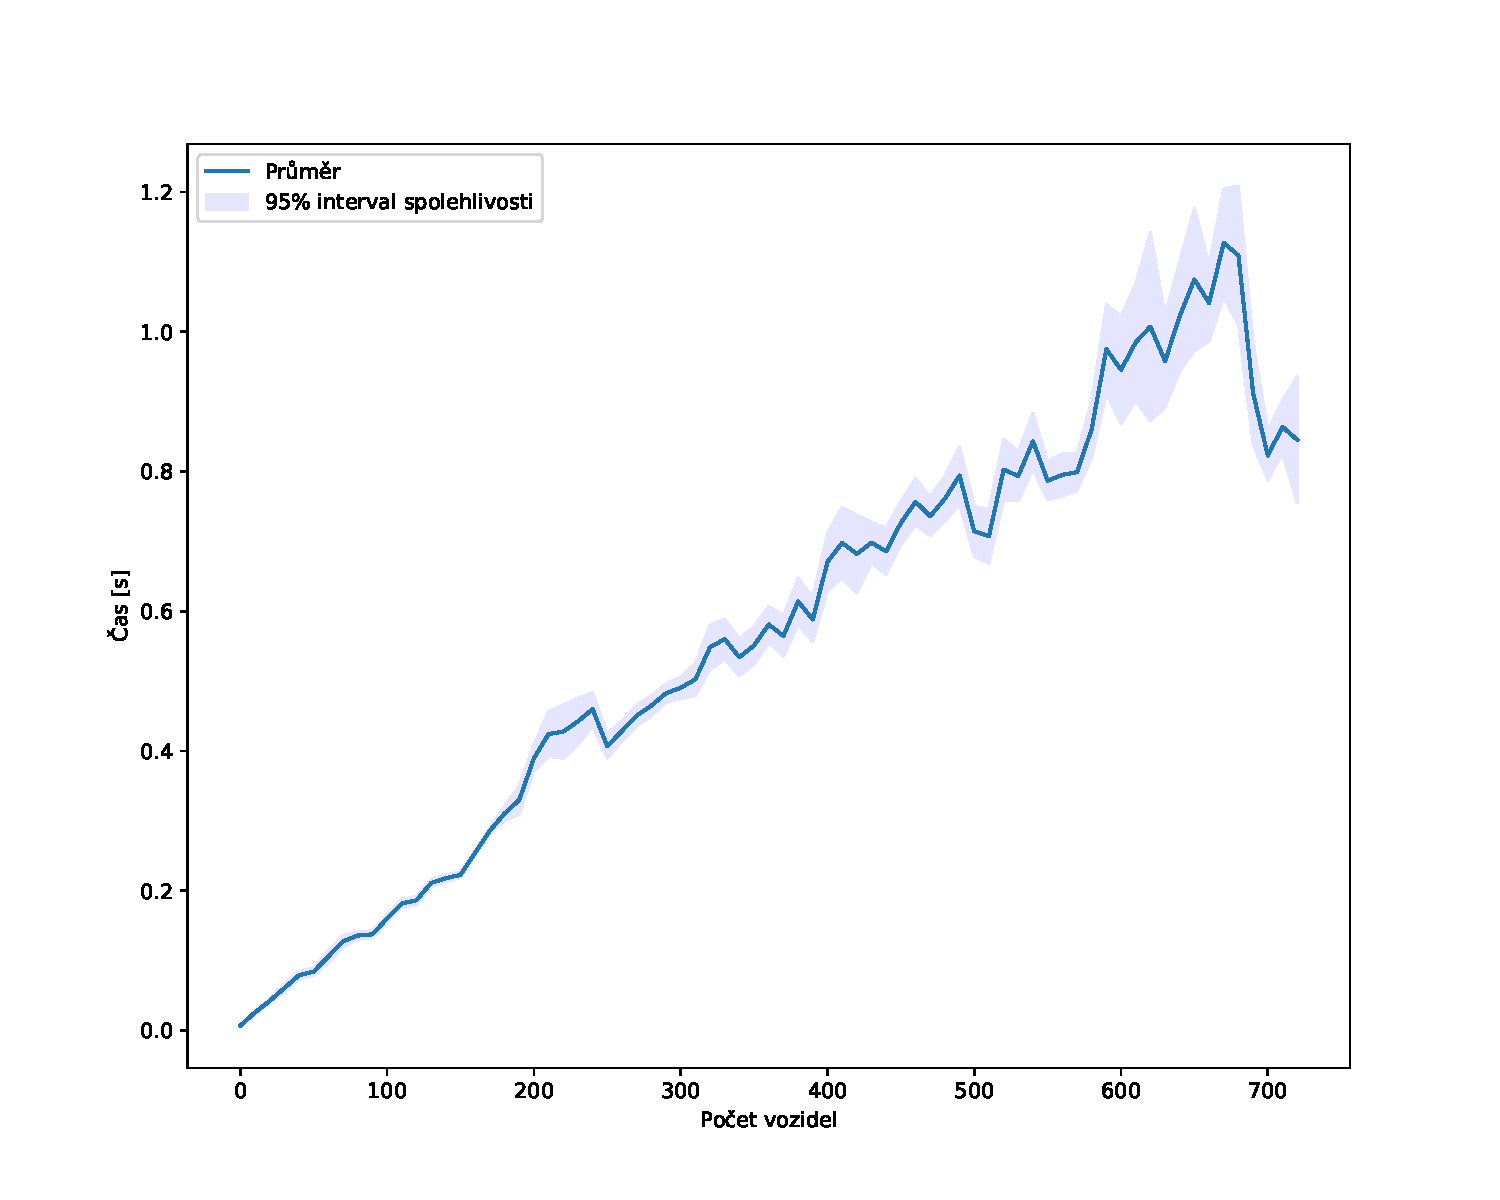
\includegraphics[width=0.7\linewidth]{../img/file_process_time}
  \caption{Průměrný čas zpracovávání daného počtu vozidel ze všech souborů se statickými daty. Světle modrá barva ohraničuje 95 \% interval spolehlivosti. Počty vozidel jsou vždy zaokrouhleny dolů na celé desítky.}
  \label{fig:file_process_time}
\end{figure}

\bigbreak

Jediné delší prodlení může nastat ve chvíli, kdy je potřeba stáhnout velké množství dodatečných informací o novém spoji. Na grafu \ref{fig:vehicle_pos_x_new_trips} je vidět, že až na jednotky vyjímek je počet nově nalezených spojů v jednom souboru nejvýše 20. Aplikace je ale naimplementována tak, aby se tyto informace stahovaly asynchroně a tedy čákání na stažení dat je co nejkratší.

\subsubsection{Konstrukce modelů}

Čtení dat potřebných pro trénování modelů z databáze, kde jsou data ze 4 dnů trvá přibližně 110 sekund. Čtení se totiž provádí komlikovaným \gls{sql} datazem uvedeným v kapitole \ref{subsection:cteni_dat}, ovšem na rychlost provedení tohoto dotazu i konstrukce modelů celkem neklademe žádné časové nároky, protože přepočítávání modelů je plánováno na čas nejmenšího zatížení systému, což bývá typicky v noci, kdy máme několik hodin pro výpočet.

\bigbreak

Dále ověřme, že výsledek dotazu nezahltí pamětˇ počítače, dotaz sice umožnˇuje čtení dat po stránkách, ale v implementaci se tato vlastnost nevyužívá. Určení velikosti objektu jazyka Python3 v paměti počítače není úplně trivální úloha, dobrý odhad nám, ale poskytne objektu na disk pomocí knihovny \verb-pickle-. Takto uložený objekt zabírá necelých 10 MB prostoru na disku.

\bigbreak



\section{Evaluace výsledků}

\subsection{Sestrojení modelů}

Po využití testovacích dat vzorků poloh vozidel zaznamenaných ve dnech 20.--24. února 2020 bylo podle krytérií, kterými jsou zejména vzdálenost zastávek a počet vzorků mezi nimi, sestrojeno celkem 1106 polynomiálních modelů. Z toho je 847 modelů pro pracovní dny, které jsou nejdůležitější. Přičemž celkový počet párů zastávek je 7230, ale zastávek ve vzdálenosti 1500 metrů\footnote{zvolená minimální vzdálenost mezi zastávkama, mezi kterýma má ještě smysl odhadovat zpoždění} je pouze 2142. Z toho vychází, že u 40 \% dvojic zastávek je dostatek dat, aby dával výpočet modelu smysl.

\bigbreak

U zbylých dvojic zastávek se využívá lineární model.

\subsection{Odhady zpoždění}

Z toho jak jsou definovány požadavky řešení v kapitole \ref{subsubsection:kvalitativni_pozadavky} pro změření kvality výsledků stačí porovnávat odhad zpoždění lineárního (původního) modelu a nového polynomiálního modelu. Přičemž odhad je lepší pokud má sekvence odhadů  z celé jízdy mezi dvojcí zastávek menší rozptyl.

\bigbreak

Podívejme se tedy na porovnání odhadů zpoždění novými modely profilů jízd se stávajícím řešení pracujícím s předpokladem, že vozidla jedou celou trasu mezi dvěma zastávkami konstantní rychlostí.

\bigbreak

Evaluaci výsledků budeme provádět s daty sesbíranými 20. 2. 2020, které použijeme jako trénovací data a s daty sesbíranými 21. 2. 2020, které použijeme jako testovací data. Toto je standardní postup pro hodnocení úspěšnosti predikcí modelů ve světě strojového učení. Modely nemohou být testovány na stejných datech jako na kterých byly trénovány, protože kdyby se trénovalo i testovalo na stejných datech, model by nemusel nic predikovat, ale stačilo by, aby si jen "zapamatoval" hodnotu z množiny trénovacích dat.

\bigbreak


\chapter*{Závěr}
\addcontentsline{toc}{chapter}{Závěr}


Nejprve jsme se seznámili s~daty a~po jejich analýze se zkušeností a~intuicí s~vývojem dopravních situací jsme zvážili, zda je problém možné řešit a~jaký dopad by mohl mít v~reálném nasazení. Ačkoli požadavek na zlepšení odhadu nebo i~předpovědi zpoždění vozidel \gls{vhd} se zdá naprosto přirozený, žádné z~dosud existujících řešení zpracovávající real-time data se o~nic takového nepokouší. O~to víc je to překvapující s~přihlédnutím k~množství cestujících v~Praze i~jinde na světě.


\bigbreak

Dále jsme analyzovali jiné nástroje v~České republice vizualizující polohy vozidel a~definovali jsme problém, Následně jsme si zadali samotné požadavky na dílo.

\bigbreak

Navrhli jsme procesy zpracování vstupních dat a~jejich následné využití k~pravděpodobnostnímu odhadu zpoždění. Také jsme navrhli algoritmus, který se používá v~této práci pro odhad zpoždění a~algoritmus, který řeší komplikovanější situace, než s~jakými jsme se setkali v~pražské dopravní síti. Ačkoli tento návrhovaný algoritmus neimplementujeme, může sloužit jako základní kámen pro další výzkum a~obdobné aplikace. Součástí návrhu je design front-endu aplikace a~databázové struktury.


\bigbreak

Zdrojový kód aplikace jsme zdokumentovali jako součást kódu a~logiku běhu softwaru jsme popsali v~kapitole implementace. Rozděleně jsou popsány části zpracování dat, výpočet modelů sloužících k~odhadu zpoždění a~server-klient vizualizační aplikace. Pro serverovou část jsme popsali, jak se k~ní připojit v~případě vývoje jiné klientské aplikace.


\bigbreak

Na závěr jsme celou aplikaci otestovali, a~to od jednotlivých funkcí tříd až po aplikaci jako celek. Testování funkcí jsme provedli pomocí unit testů. Složitější celky včetně správné funkčnosti databáze jsme otestovali pomocí integračních testů. Server byl podroben zátěžovým testům, kdy jsme jej dotazovali velkým množstvím paralelních dotazů. Rychlost zpracování dat byla měřena v~bodě maximálního vytížení.


\bigbreak

Velkou část testování tvořilo ověření výsledků, tedy odhadů zpoždění. Z~kterého vyplynulo, že v~nezanedbatelném množství případů došlo opravdu k~výraznému zlepšení. Zvolená metoda se však nedá uplatnit ve všech případech, a~to zejména z~důvodu, že klasické řešení dosahuje dobrých výsledků a~není tam tedy prostor ke zlepšení.


\section*{Návrhy na zlepšení}

Tak jak je aplikace napsána, je schopná samostatného běhu, avšak protože nemůžeme otestovat aplikaci v~dlouhodobém nasazení je potřeba vyřešit několik problémů s~tím souvisejících. První problém může být objem dat, které je potřeba skladovat, a~tím zpomalující se reakční doba databáze. V~takovém případě navrhujeme historická data skladovat na odděleném místě od databáze, kde ukládáme aktuální data, a~do které se dotazuje server. Dále je potřeba také určit správnou periodu přepočítání modelů a~jak vybírat data, která pro počítání modelů použít.


\bigbreak

Protože jsme při návrhu aplikace rozhodli rozdělit vstupní data pro výpočet modelů do dvou podmnožin -- zaznamená v~pracovní den a~víkendový den. Nabízí se vylepšení do dní pracovního volna započítat i~státní svátky. Nebo ještě lépe pro výpočet jednoho modelu použít data jen z~jednoho dne v~týdnu a~vázat tak model na konkrétní den v~týdnu.
\bigbreak


Vzhledem k~tomu, že v~této práci pracujeme s~geografickými daty, bylo by vhodnější použít jinou \gls{sql} databázi, protože MySQL databáze není příliš uzpůsobená pro ukládání tohoto typu dat. Vhodnější implementace databáze se nabízí PostgreSQL\footnote{\url{https://www.postgresql.org}} s~rozšířením PostGIS\footnote{\url{https://postgis.net}}.

\bigbreak

Jako poslední návrh na zlepšení je samotné vylepšení modelů popisujících profily jízd. Ať už zvolením modelu jiného typu nebo zcela odlišného přístupu k~problému. Aplikace je nastavena tak, aby se při vylepšování modelů nemusely měnit jiné části aplikace.


%%% Seznam použité literatury
%%% Seznam použité literatury (bibliografie)
%%%
%%% Pro vytváření bibliografie používáme bibTeX. Ten zpracovává
%%% citace v textu (např. makro \cite{...}) a vyhledává k nim literaturu
%%% v souboru literatura.bib.
%%%
%%% Příkaz \bibliographystyle určuje, jakým stylem budou citovány odkazy
%%% v textu. V závorce je název zvoleného souboru .bst. Styly plainnat
%%% a unsrt jsou standardní součástí latexových distribucí. Styl czplainnat
%%% je dodáván s touto šablonou a bibTeX ho hledá v aktuálním adresáři.

\bibliographystyle{czplainnat}    %% Autor (rok) s českými spojkami
% \bibliographystyle{plainnat}    %% Autor (rok) s anglickými spojkami
% \bibliographystyle{unsrt}       %% [číslo]

\renewcommand{\bibname}{Seznam použité literatury}

%%% Vytvoření seznamu literatury. Pozor, pokud jste necitovali ani jednu
%%% položku, seznam se automaticky vynechá.

\bibliography{literatura}

%%% Kdybyste chtěli bibliografii vytvářet ručně (bez bibTeXu), lze to udělat
%%% následovně. V takovém případě se řiďte normou ISO 690 a zvyklostmi v oboru.

% \begin{thebibliography}{99}
%
% \bibitem{lamport94}
%   {\sc Lamport,} Leslie.
%   \emph{\LaTeX: A Document Preparation System}.
%   2. vydání.
%   Massachusetts: Addison Wesley, 1994.
%   ISBN 0-201-52983-1.
%
% \end{thebibliography}


%%% Obrázky v~bakalářské práci
%%% (pokud jich je malé množství, obvykle není třeba seznam uvádět)
\listoffigures

%%% Tabulky v~bakalářské práci (opět nemusí být nutné uvádět)
%%% U~matematických prací může být lepší přemístit seznam tabulek na začátek práce.
\listoftables

%%% Použité zkratky v~bakalářské práci (opět nemusí být nutné uvádět)
%%% U~matematických prací může být lepší přemístit seznam zkratek na začátek práce.
% \chapwithtoc{Seznam použitých zkratek}
\printnoidxglossaries

%%% Přílohy k~bakalářské práci, existují-li. Každá příloha musí být alespoň jednou
%%% odkazována z~vlastního textu práce. Přílohy se číslují.
%%%
%%% Do tištěné verze se spíše hodí přílohy, které lze číst a~prohlížet (dodatečné
%%% tabulky a~grafy, různé textové doplňky, ukázky výstupů z~počítačových programů,
%%% apod.). Do elektronické verze se hodí přílohy, které budou spíše používány
%%% v~elektronické podobě než čteny (zdrojové kódy programů, datové soubory,
%%% interaktivní grafy apod.). Elektronické přílohy se nahrávají do SISu a~lze
%%% je také do práce vložit na CD/DVD. Povolené formáty souborů specifikuje
%%% opatření rektora č. 72/2017.
\appendix
\chapter{Přílohy}

\section{První příloha}

K elektronické verzi této práce jsou přiloženy zdrojové kódy celé popsané aplikace včetně testů, vstupní statická data a vytvořené modely profilů tras jízd.

\openright
\end{document}
